%
% main.tex -- Paper zum Thema <thema>
%
% (c) 2018 Hansruedi Patzen, Hochschule Rapperswil
%
\chapter{H"oherdimensionales Lorenzsystem\label{chapter:lorenz2}}
\lhead{H"oherdimensionales Lorenzsystem}
\begin{refsection}
\chapterauthor{Hansruedi Patzen}

Auf das dreidimensionale Lorenzsystem wurde bereits in 
\cref{section:lorenz-modell} sowie in \cref{chapter:lorenz} detailliert 
eingegangen. Trotzdem wollen wir nochmals die f"ur das Lorenz-Modell relevanten 
Grundgleichungen
\begin{equation}
	\begin{aligned}
	\frac{\partial\Delta\psi}{\partial t}
	&=
	\nu\Delta^2\psi 
	+c\frac{\partial\vartheta}{\partial x}
	-\frac{\partial(\psi,\Delta\psi)}{\partial(x,y)}
	\\
	\frac{\partial\vartheta}{\partial t}
	&=
	\kappa\Delta\vartheta
	+ \frac{T_0}{\pi}\frac{\partial\psi}{\partial x}
	- \frac{\partial(\psi,\vartheta)}{\partial(x,y)}
	\end{aligned}
	\label{equation:lorenz2:base}
\end{equation}
genauer analysieren. Dank einer geschickten Wahl von Basisfunktionen
\begin{equation*}
	\sin(ax)\sin(y),
	\qquad
	\cos(ax)\sin(y)
	\qquad\text{und}\qquad
	\sin(2y)
\end{equation*}
und einigen Vereinfachungen, hatten wir es geschafft, das System auf drei 
gew"ohnliche Differentialgleichungen
\begin{equation*}
	\begin{aligned}
	\dot X(t)
	&=
	-\nu(a^2+1)X(t)
	+\frac{ac}{a^2+1}Y(t)
	\\
	\dot Y(t)
	&=
	\frac{aT_0}{\pi}X(t)
	-(a^2+1)\kappa Y(t)
	-aX(t)Z(t)
	\\
	\dot Z(t)
	&=
	-4\kappa Z(t)
	+\frac{a}{2}X(t)Y(t)
	\end{aligned}
\end{equation*}
zu reduzieren, welche unser dreidimensionale Lorenzsystem beschreiben.

In diesem Kapitel wollen wir nun dieses mit Separationsverfahren gefunden 
L"osungen, welche unsere Basisfunktionen bilden erweitern. Diese neuen 
Basisfunktionen sollen es uns erm"oglichen auch Terme die wir bisher bei 
unserer L"osung vernachl"assigt haben miteinzubeziehen. Dies f"uhrt uns dann 
schlussendlich wieder zu einem Lorenzsystem, welches aber nicht mehr 
dreidimensional sondern eben h"oherdimensional ist. Bis es soweit ist und wir 
die Resultate in \cref{section:lorenz2:numeric-solution} begutachten k"onnen, 
m"ussen wir erst ein paar Dinge zur Notation und allgemeinen Formeln in 
\cref{section:lorenz2:einstieg} kl"aren. Danach machen wir uns auf die Suche 
neuer Basisfunktionen in \cref{section:lorenz2:basic_function} und generieren 
nach Einsetzen und Vereinfachen in \cref{section:lorenz2:ho-model} die zum 
l"osen unserer neuen h"oherdimensionalen Lorenzsystems ben"otigten 
gew"ohnlichen Differentialgleichungen. \Cref{section:lorenz2:4degreelorenz} 
zeigt uns am konkreten Beispiel eines Lorenzsystem vierten Grades, was alles 
verloren geht, wenn man Terme einfach vernachl"assigt.

\section{Einf"uhrung}
\rhead{Einf"uhrung}

Bevor wir uns auf die Suche nach Basisfunktionen machen, folgen hier ein paar 
Angaben zu den in diesem Kapitel verwendeten Notation und einigen grundlegenden 
Funktionen und Umformungen, welche sp"ater verwendet werden, ein kleiner 
``Teaser'' zu dem was uns noch erwartet sozusagen.

\subsection{Notation}
Die verwendete Notation entspricht grunds"atzlich derjenigen, welche man 
bereits aus anderen mathematischen B"uchern kennt. Einzig die Verwendung der 
sogenannten Multi-Index-Notationen k"onnte f"ur einige Leser zu Unklarheiten 
f"uhren, daher hier eine kurze Einf"uhrung.

Unter der Multi-Index-Notation versteht man einen Index, der einem 
$n$-Tupel
\begin{equation*}
	\alpha = (\alpha_1, \alpha_2, \dotsc, \alpha_n) \qquad \alpha_k \in 
	\mathbb{N}_{0}
\end{equation*}
entspricht. Zur klaren Unterscheidung zu normalen Indexen, wird meist ein 
griechischer Buchstabe verwendet. Multi-Indexe haben zudem die Eigenschaft, 
dass ihr absoluter Wert wie folgt definiert ist
\begin{equation*}
	|\alpha| = \alpha_1 + \alpha_2 + \dots + \alpha_n.
\end{equation*}
 
N"utzlich ist diese Notation insbesondere, wenn mit Summen gearbeitet wird. So 
kann mittels einer Forderung wie beispielsweise $|\alpha| = k$, die Summe
\begin{equation}
	\sum_{k = 0}^{\infty}\sum_{l = 0}^{k}a_{l, k - l}
	\label{equation:lorenz2:doublesum}
\end{equation}
vereinfacht werden zu
\begin{equation}
	\sum_{k = 0}^{\infty}a_{\alpha} \qquad |\alpha| = k.
	\label{equation:lorenz2:mmsum}
\end{equation}
M"oglich ist dies, da $|\alpha| = k$ f"ur alle Kombinationen der verschiedenen 
$|\alpha_m|$ gilt. Zum Beispiel ist $|\alpha| = k = 2$ f"ur $2$-Tupel 
Multi-Indexe
\begin{align*}
	\alpha &= (0, 2), \\
	\alpha &= (1, 1), \\
	\alpha &= (2, 0)
\end{align*}
erf"ullt, was genau dem in \cref{equation:lorenz2:doublesum} f"ur $k = 2$ 
geforderten Index-Tupel $(l, k - l)$ entspricht.

\subsection{Formel Sammelserum}
Einige Umformungen, die wir in den n"achsten Abschnitten vornehmen werden, 
verwenden teilweise nicht ganz gel"aufige Funkionen. Damit nicht immer gleich 
Wikipedia bem"uht werden muss, werden diese hier in einem kleinen 
Formel Sammelserum zusammengestellt.

Die Signum-Funktion (kurz $\sgn(x)$):
\begin{equation}
\sgn(x) =
\begin{cases*}
1 & f"ur x > 0 \\
0 & f"ur x = 0 \\
-1 & f"ur x < 0
\end{cases*}
\label{equation:lorenz2:signum}
\end{equation}

Betragsfunktion (kurz $|x|$)
\begin{equation}
|x| =
\begin{cases*}
x & f"ur x $\geq$ 0 \\
-x & f"ur x < 0
\end{cases*}
\label{equation:lorenz2:absfunction}
\end{equation}

Sinus und Kosinus eines absoluten Wertes (\cref{equation:lorenz2:absfunction}):
\begin{equation}
\begin{split}
\sin(|x|) &= \sgn(x)\sin(x) \qquad \Leftrightarrow \qquad \sin(x) = 
\sgn(x)\sin(|x|)
\\
\cos(|x|) &= \cos(x)
\end{split}
\label{equation:lorenz2:sincosabs}
\end{equation}

Produkte von Sinus und Kosinus Kombinationen:
\begin{align*}
\cos(x)\sin(y) &= \frac{1}{2} \left(\sin(x + y) - \sin(x - y)\right)
\\
\sin(x)\cos(y) &= \frac{1}{2} \left(\sin(x - y) + \sin(x + y)\right)
\\
\sin(x)\sin(y) &= \frac{1}{2} \left(\cos(x - y) - \cos(x + y)\right)
\\
\cos(x)\cos(y) &= \frac{1}{2} \left(\cos(x - y) + \cos(x + y)\right)
\end{align*}

\section{Erweiterung der Basisfunktionen\label{section:lorenz2:basic_function}}
Die Suche neuer Basisfunktionen beginnt mit denjenigen, die bereits 
in \cref{skript:funktionsauswahl} erw"ahnt sind. Bei genauerer Betrachtung 
stellt man fest, dass diese auch ein wenig anders geschrieben werden k"onnen:
\begin{align*}
\sin(ax)\sin(y) &= \sin(1ax)\sin(1y),\\
\cos(ax)\sin(y) &= \cos(1ax)\sin(1y),\\
\sin(2y) &= \cos(0ax)\sin(2y).
\end{align*}
Nun f"ugen wir ein paar zus"atzliche, auf den ersten Blick etwas nutzlose
Gleichungen hinzu:
\begin{align*}
0 &= \sin(0ax)\sin(2y) \\
\sin(ax)\sin(y) &= \sin(1ax)\sin(1y)\\
0 &= \sin(2ax)\sin(0y) \\
\sin(2y) &= \cos(0ax)\sin(2y)\\
\cos(ax)\sin(y) &= \cos(1ax)\sin(1y)\\
0 &= \cos(2ax)\sin(0y)\\
\end{align*}
Daraus l"asst sich nun das Muster
\begin{equation}
\begin{split}
\sin(\alpha_1 ax)\sin(\alpha_2 y) \\
\cos(\alpha_1 ax)\sin(\alpha_2 y)
\end{split}
\label{equation:lorenz2:basic-functions}
\end{equation}
erkennen, wobei $\alpha_1$ und $\alpha_2$ Teile eines Multi-Indices sind und 
die Bedingung $|\alpha| = k = 2$ erf"ullen.

F"ur unser dreidimensionales Modell hatten wir also Basisfunktionen zweiten 
Grades ($k = 2$) gefunden. Mit den neuen Funktionen k"onnen wir aber nicht nur 
die uns bekannten generieren, sondern diese auch noch erweitern indem wir den 
Grad $k$ variieren.

Leicht zu erkennen ist, dass f"ur $k = 0$ nur die $0$-Funktion 
"ubrig bleibt, da einzig das $(0, 0)$-Tupel die Bedingung $|\alpha| = 0$ 
erf"ullt. $k = 1$ generiert die beiden Tupel $(0, 1)$ und $(1, 0)$, womit die 
Funktion $\sin(y)$ "ubrig bleibt. Somit k"onnen wir Grad $k \geq 1$ 
voraussetzen. Damit wird auch gleich das Problem einer m"oglichen Division 
durch $0$ elegant umgangen, wie wir sp"ater sehen werden.

\section{H"oherdimensionales Lorenzsystem\label{section:lorenz2:ho-model}}
\rhead{Lorenz-Modell h"oherer Ordnung}
Nun nehmen wir als/ die Grundgleichungen aus 
\cref{skript:lorenzausgangsgleichung} und unsere neuen Basisfunktionen aus 
\cref{equation:lorenz2:basic-functions} und bauen daraus ein 
h"oherdimensionales Lorenzsystem.

Als ersten Schritt erweitern wir unsere in \cref{skript:psiansatz} und 
\cref{skript:thetaansatz} gefundenen L"osungen und erhalten
\begin{equation}
\psi(x,y,t) =
\sum_{k = 1}^{\infty}
a_{\alpha}(t)
\sin(\alpha_1 ax) \sin(\alpha_2 y)
\qquad |\alpha| = k,
\label{equation:lorenz2:extendedpsi}
\end{equation}
sowie
\begin{equation}
\vartheta(x,y,t) =
\sum_{k = 1}^{\infty}
b_{\alpha}(t)
\cos(\alpha_1 ax) \sin(\alpha_2 y)
\qquad |\alpha| = k.
\label{equation:lorenz2:extendedtheta}
\end{equation}

Als n"achstes betrachten wir die \cref{skript:lorenzausgangsgleichung}
\begin{align*}
\frac{\partial\Delta\psi}{\partial t}
&=
\nu\Delta^2\psi 
+c\frac{\partial\vartheta}{\partial x}
-\frac{\partial(\psi,\Delta\psi)}{\partial(x,y)},
\\
\frac{\partial\vartheta}{\partial t}
&=
\kappa\Delta\vartheta
+ \frac{T_0}{\pi}\frac{\partial\psi}{\partial x}
- \frac{\partial(\psi,\vartheta)}{\partial(x,y)}.
\end{align*}
Statt einfach Terme zu ersetzen, macht es Sinn, systematisch vorzugehen. Es ist 
leicht zu erkennen, dass wir sowohl partielle Ableitungen nach $x$ als auch $y$ 
brauchen werden. Daher fangen wir an, uns Bausteine zurechtzulegen indem wir 
die \cref{equation:lorenz2:extendedpsi,equation:lorenz2:extendedtheta} 
zwei Mal je nach $x$ und $y$ ableiten.

F"ur $\psi(x,y,t)$ erhalten wir
\begin{align*}
\frac{\partial\psi}{\partial x}
&=
a
\sum_{k = 1}^{\infty}
\alpha_1
a_{\alpha}(t)
\cos(\alpha_1 ax) \sin(\alpha_2 y)
&&|\alpha| = k
\\
\frac{\partial\psi}{\partial y}
&=
\sum_{k = 1}^{\infty}
\alpha_2
a_{\alpha}(t)
\sin(\alpha_1 ax) \cos(\alpha_2 y)
&&|\alpha| = k
\\
\frac{\partial^2\psi}{\partial x^2}
&=
-
a^2
\sum_{k = 1}^{\infty}
\alpha_1^2
a_{\alpha}(t)
\sin(\alpha_1 ax) \sin(\alpha_2 y)
&&|\alpha| = k
\\
\frac{\partial^2\psi}{\partial y^2}
&=
-
\sum_{k = 1}^{\infty}
\alpha_2^2
a_{\alpha}(t)
\sin(\alpha_1 ax) \sin(\alpha_2 y)
&&|\alpha| = k
\end{align*}
und f"ur $\vartheta(x,y,t)$
\begin{align*}
\frac{\partial\vartheta}{\partial x}
&=
-
a
\sum_{k = 1}^{\infty}
\alpha_1
b_{\alpha}(t)
\sin(\alpha_1 ax) \sin(\alpha_2 y)
&&|\alpha| = k
\\
\frac{\partial\vartheta}{\partial y}
&=
\sum_{k = 1}^{\infty}
\alpha_2
b_{\alpha}(t)
\cos(\alpha_1 ax) \cos(\alpha_2 y)
&&|\alpha| = k
\\
\frac{\partial^2\vartheta}{\partial x^2}
&=
-
a^2
\sum_{k = 1}^{\infty}
\alpha_1^2
b_{\alpha}(t)
\cos(\alpha_1 ax) \sin(\alpha_2 y)
&&|\alpha| = k
\\
\frac{\partial^2\vartheta}{\partial y^2}
&=
-
\sum_{k = 1}^{\infty}
\alpha_2^2
b_{\alpha}(t)
\cos(\alpha_1 ax) \sin(\alpha_2 y)
&&|\alpha| = k.
\end{align*}

Damit haben wir alles zusammen um den einfachen Laplace Operator $\laplace$ 
f"ur $\psi(x,y,t)$
\begin{align*}
\laplace\psi
&= 
\frac{\partial^2\psi}{\partial x^2}
+
\frac{\partial^2\psi}{\partial y^2}
\\
&=
-
a^2
\sum_{i = 1}^{\infty}
\gamma_1^2
a_{\gamma}(t)
\sin(\gamma_1 ax) \sin(\gamma_2 y)
-
\sum_{j = 1}^{\infty}
\delta_2^2
a_{\delta}(t) 
\sin(\delta_1 ax) \sin(\delta_2 y)
&&|\gamma| = i, |\delta| = j
\\
&=
-
\sum_{k = 1}^{\infty}
\left(\alpha_1^2 a^2 + \alpha_2^2 \right)
a_{\alpha}(t)
\sin(\alpha_1 ax) \sin(\alpha_2 y)
&&|\alpha| = k
\end{align*}
und $\vartheta(x,y,t)$
\begin{align*}
\laplace\vartheta &= 
\frac{\partial^2\vartheta}{\partial x^2}
+
\frac{\partial^2\vartheta}{\partial y^2} \\
&=
-
a^2
\sum_{i = 1}^{\infty}
\alpha_1^2
b_{\gamma}(t)
\cos(\gamma_1 ax) \sin(\gamma_2 y)
-
\sum_{j = 1}^{\infty}
\delta_2^2
b_{\delta}(t)
\cos(\delta_1 ax) \sin(\delta_2 y)
&&|\gamma| = i, |\delta| = j
\\
&=
-
\sum_{k = 1}^{\infty}
\left(\alpha_1^2 a^2 + \alpha_2^2\right)
b_{\alpha}(t)
\cos(\alpha_1 ax) \sin(\alpha_2 y)
&&|\alpha| = k
\end{align*}
aufzul"osen. In \cref{equation:lorenz2:extendedpsi} brauchen wir zudem 
$\laplace^2\psi(x,y,t)$. Daf"ur ben"otigen wir die zweifachen Ableitungen von 
$\laplace\psi(x,y,t)$ nach $x$ und $y$
\begin{align*}
\frac{\partial\laplace\psi}{\partial x} &=
-
a
\sum_{k = 1}^{\infty}
\alpha_1
\left(\alpha_1^2 a^2 + \alpha_2^2 \right)
a_{\alpha}(t)
\cos(\alpha_1 ax) \sin(\alpha_2 y)
&&|\alpha| = k
\\
\frac{\partial^2\laplace\psi}{\partial x^2}
&=
a^2
\sum_{k = 1}^{\infty}
\alpha_1^2
\left(\alpha_1^2 a^2+\alpha_2^2\right)
a_{\alpha}(t)
\sin(\alpha_1 ax) \sin(\alpha_2 y)
&&|\alpha| = k
\\
\frac{\partial\laplace\psi}{\partial y}
&=
-
\sum_{k = 1}^{\infty}
\alpha_2
\left(\alpha_1^2 a^2 + \alpha_2^2 \right)
a_{\alpha}(t)
\sin(\alpha_1 ax) \cos(\alpha_2 y)
&&|\alpha| = k
\\
\frac{\partial^2\laplace\psi}{\partial y^2}
&=
\sum_{k = 1}^{\infty}
\alpha_2^2
\left(\alpha_1^2 a^2+\alpha_2^2\right)
a_{\alpha}(t)
\sin(\alpha_1 ax) \sin(\alpha_2 y)
&&|\alpha| = k
\end{align*}
und k"onnen dann
\begin{align*}
\laplace^2\psi
&= 
\frac{\partial^2\laplace\psi}{\partial x^2} + 
\frac{\partial^2\laplace\psi}{\partial y^2} \\
&=
a^2
\sum_{i = 1}^{\infty}
\gamma_1^2
\left(\gamma_1^2 a^2+\gamma_2^2\right)
a_{\gamma}(t)
\sin(\gamma_1 ax) \sin(\gamma_2 y)
\\
&\phantom{={}}
+
\sum_{j = 1}^{\infty}
\delta_2^2
\left(\delta_1^2 a^2+\delta_2^2\right)
a_{\delta}(t)
\sin(\delta_1 ax) \sin(\delta_2 y)
&&|\gamma| = i, |\delta| = j
\\
&=
\sum_{k = 1}^{\infty}
\left(\alpha_1^2 a^2+\alpha_2^2\right)^2
a_{\alpha}(t)
\sin(\alpha_1 ax) \sin(\alpha_2 y)
&&|\alpha| = k
\end{align*}
zusammenbauen.

Bei einigen werden sich bei den Gleichungen f"ur die Laplace Operatoren beim 
Addieren zweier unendlicher Summen wahrscheinlich die Nackenhaare hochgestellt 
haben. Diese Umformung sei uns aber erlaubt, da wir davon ausgehen m"ussen, 
dass die einzelnen Serien konvergent sind. Zudem h"alt uns nichts davon ab, die 
Indexe der beiden unabh"angigen Summen so umzubenennen, dass diese 
"Ubereinstimmen. Damit ist klar, dass die gleichen Basisfunktionen generiert 
werden und die Summen somit vereinfacht werden k"onnen.

Mit unseren bisherigen Bausteinen haben wir jetzt fast alles zusammen, um 
\cref{skript:lorenzausgangsgleichung} aufzul"osen. Einzig die 
Funktionsdeterminanten fehlen noch, was auch dem haarigen Teil der Gleichung 
entspricht, was uns erst die Kopplung der beiden Terme beschert.

Beginnen wir also damit die erste Funktionsdeterminante
\begin{align*}
\frac{\partial(\psi, \laplace\psi)}{\partial(x,y)}
&=
\frac{\partial\psi}{\partial x}
\frac{\partial\laplace\psi}{\partial y}
-
\frac{\partial\psi}{\partial y}
\frac{\partial\laplace\psi}{\partial x}
\\
&=
\left(
a
\sum_{i = 1}^{\infty}
\gamma_1
a_{\gamma}(t)
\cos(\gamma_1 ax) \sin(\gamma_2 y)
\right)
\left(
-
\sum_{j = 1}^{\infty}
\delta_2
\left(\delta_1^2 a^2 + \delta_2^2 \right)
a_{\delta}(t)
\sin(\delta_1 ax) \cos(\delta_2 y)
\right)
\\
&\phantom{={}}
-
\left(
\sum_{q = 1}^{\infty}
\xi_2
a_{\xi}(t)
\sin(\xi_1 ax) \cos(\xi_2 y)
\right)
\left(
-
a
\sum_{r = 1}^{\infty}
\eta_1
\left(\eta_1^2 a^2 + \eta_2^2 \right)
a_{\eta}(t)
\cos(\eta_1 ax) \sin(\eta_2 y)
\right)
\\
&|\gamma| = i, |\delta| = j, |\xi| = q, |\eta| = r
\\
&=
-
a
\sum_{i = 1}^{\infty}
\gamma_1
a_{\gamma}(t)
\sum_{j = 1}^{\infty}
\delta_2
\left(\delta_1^2 a^2 + \delta_2^2 \right)
a_{\delta}(t)
\cos(\gamma_1 ax) \sin(\gamma_2 y)
\sin(\delta_1 ax) \cos(\delta_2 y)
\\
&\phantom{={}}
+
a
\sum_{q = 1}^{\infty}
\xi_2
a_{\xi}(t)
\sum_{r = 1}^{\infty}
\eta_1
\left(\eta_1^2 a^2 + \eta_2^2 \right)
a_{\eta}(t)
\sin(\xi_1 ax) \cos(\xi_2 y)
\cos(\eta_1 ax) \sin(\eta_2 y)
\\
&=
-
a
\sum_{i = 1}^{\infty}
\gamma_1
a_{\gamma}(t)
\sum_{j = 1}^{\infty}
\delta_2
\left(\delta_1^2 a^2 + \delta_2^2 \right)
a_{\delta}(t) 
\cos(\gamma_1 ax) \sin(\gamma_2 y)
\sin(\delta_1 ax) \cos(\delta_2 y)
\\
&\phantom{={}}
+
a
\sum_{j = 1}^{\infty}
\delta_2
a_{\delta}(t)
\sum_{i = 1}^{\infty}
\gamma_1
\left(\gamma_1^2 a^2 + \gamma_2^2 \right)
a_{\gamma}(t)
\sin(\delta_1 ax) \cos(\delta_2 y)
\cos(\gamma_1 ax) \sin(\gamma_2 y)
\\
&=
a
\sum_{i = 1}^{\infty}
\gamma_1
a_{\gamma}(t)
\sum_{j = 1}^{\infty}
\delta_2
\left(
a^2 \left(\gamma_1^2 - \delta_1^2 \right)
+ \left(\gamma_2^2 - \delta_2^2 \right)
\right)
a_{\delta}(t)
\\[-2.5ex]
&\phantom{=abbbbb\sum\sum.....{}}
\cdot
\cos(\gamma_1 ax) \sin(\gamma_2 y)
\sin(\delta_1 ax) \cos(\delta_2 y)
\\
&=
\frac{a}{4}
\sum_{i = 1}^{\infty}
\gamma_1
a_{\gamma}(t)
\sum_{j = 1}^{\infty}
\delta_2
\left(
a^2 \left(\gamma_1 - \delta_1 \right)\left( \gamma_1 + \delta_1 \right)
+ \left(\gamma_2 - \delta_2 \right)\left( \gamma_2 + \delta_2 \right)
\right)
a_{\delta}(t)
\\[-2.5ex]
&\phantom{=abbbbb\sum\sum.....{}}
\cdot
\Big(
\sin((\gamma_1 + \delta_1) ax)\sin((\gamma_2 + \delta_2) y)
\\[-1.0ex]
&\phantom{=abbbbb\sum\sum.....{}}
+
\sin((\gamma_1 + \delta_1) ax)\sin((\gamma_2 - \delta_2) y)
\\[-1.0ex]
&\phantom{=abbbbb\sum\sum.....{}}
-
\sin((\gamma_1 - \delta_1) ax)\sin((\gamma_2 + \delta_2) y)
\\[-1.0ex]
&\phantom{=abbbbb\sum\sum.....{}}
-
\sin((\gamma_1 - \delta_1) ax)\sin((\gamma_2 - \delta_2) y)
\Big)
\\
&=
\frac{a}{4}
\sum_{i = 1}^{\infty}
\gamma_1
a_{\gamma}(t)
\sum_{j = 1}^{\infty}
\delta_2
\left(
a^2 \left(\gamma_1 - \delta_1 \right)\left( \gamma_1 + \delta_1 \right)
+ \left(\gamma_2 - \delta_2 \right)\left( \gamma_2 + \delta_2 \right)
\right)
a_{\delta}(t)
\\[-2.5ex]
&\phantom{=abbbbb\sum\sum.....{}}
\cdot
\Big(
\sgn(\gamma_1 + \delta_1)\sgn(\gamma_2 + \delta_2)
\sin(|\gamma_1 + \delta_1|ax)\sin(|\gamma_2 + \delta_2|y)
\\[-1.0ex]
&\phantom{=abbbbb\sum\sum.....{}}
+
\sgn(\gamma_1 + \delta_1)\sgn(\gamma_2 - \delta_2)
\sin(|\gamma_1 + \delta_1|ax)\sin(|\gamma_2 - \delta_2|y)
\\[-1.0ex]
&\phantom{=abbbbb\sum\sum.....{}}
-
\sgn(\gamma_1 - \delta_1)\sgn(\gamma_2 + \delta_2)
\sin(|\gamma_1 - \delta_1|ax)\sin(|\gamma_2 + \delta_2|y)
\\[-1.0ex]
&\phantom{=abbbbb\sum\sum.....{}}
-
\sgn(\gamma_1 - \delta_1)\sgn(\gamma_2 - \delta_2)
\sin(|\gamma_1 - \delta_1|ax)\sin(|\gamma_2 - \delta_2|y)
\Big)
\\
&|\gamma| = i, |\delta| = j
\end{align*}
und analog dazu kann auch die zweite
\begin{align*}
\frac{\partial(\psi, \vartheta)}{\partial(x,y)}
&=
\frac{\partial\psi}{\partial x}
\frac{\partial\vartheta}{\partial y}
-
\frac{\partial\psi}{\partial y}
\frac{\partial\vartheta}{\partial x}
\\
&=
\left(
a
\sum_{i = 1}^{\infty}
\gamma_1
a_{\gamma}(t)
\cos(\gamma_1 ax) \sin(\gamma_2 y)
\right)
\left(
\sum_{j = 1}^{\infty}
\delta_2
b_{\delta}(t)
\cos(\delta_1 ax) \cos(\delta_2 y)
\right)
\\
&\phantom{={}}
-
\left(
\sum_{q = 1}^{\infty}
\xi_2
a_{\xi}(t)
\sin(\xi_1 ax) \cos(\xi_2 y)
\right)
\left(
-
a
\sum_{r = 1}^{\infty}
\eta_1
b_{\eta}(t)
\sin(\eta_1 ax) \sin(\eta_2 y)
\right)
\\
&|\gamma| = i, |\delta| = j, |\xi| = q, |\eta| = r
\\
&=\phantom{+}
a
\sum_{i = 1}^{\infty}
\gamma_1
a_{\gamma}(t)
\sum_{j = 1}^{\infty}
\delta_2
b_{\delta}(t)
\cos(\gamma_1 ax) \sin(\gamma_2 y)
\cos(\delta_1 ax) \cos(\delta_2 y)
\\
&\phantom{={}}
+
a
\sum_{q = 1}^{\infty}
\xi_2
a_{\xi}(t)
\sum_{r = 1}^{\infty}
\eta_1
b_{\eta}(t)
\sin(\xi_1 ax) \cos(\xi_2 y)
\sin(\eta_1 ax) \sin(\eta_2 y)
\\
&=\phantom{+}
a
\sum_{i = 1}^{\infty}
\gamma_1
a_{\gamma}(t)
\sum_{j = 1}^{\infty}
\delta_2
b_{\delta}(t)
\cos(\gamma_1 ax) \sin(\gamma_2 y)
\cos(\delta_1 ax) \cos(\delta_2 y)
\\
&\phantom{={}}
+
a
\sum_{i = 1}^{\infty}
\gamma_2
a_{\gamma}(t)
\sum_{j = 1}^{\infty}
\delta_1
b_{\delta}(t)
\sin(\gamma_1 ax) \cos(\gamma_2 y)
\sin(\delta_1 ax) \sin(\delta_2 y)
\\
&=
a
\sum_{i = 1}^{\infty}
a_{\gamma}(t)
\sum_{j = 1}^{\infty}
b_{\delta}(t)
\left(
\gamma_1 \delta_2
\cos(\gamma_1 ax) \sin(\gamma_2 y)
\cos(\delta_1 ax) \cos(\delta_2 y)
\right.
\\[-2.5ex]
&\phantom{=abbb\sum\sum.....{}}
\left.
+
\gamma_2 \delta_1
\sin(\gamma_1 ax) \cos(\gamma_2 y)
\sin(\delta_1 ax) \sin(\delta_2 y)
\right)	
\\
&=
\frac{a}{4}
\sum_{i = 1}^{\infty}
a_{\gamma}(t)
\sum_{j = 1}^{\infty}
b_{\delta}(t)
\left(
\gamma_1 \delta_2
\left(
\cos((\gamma_1 - \delta_1)ax)\sin((\gamma_2 + \delta_2)y)
\right.
\right.
\\[-2.5ex]
&\phantom{=abbb\sum\sum.....{}}
+\cos((\gamma_1 - \delta_1)ax)\sin((\gamma_2 - \delta_2)y)
\\[-1.0ex]
&\phantom{=abbb\sum\sum.....{}}
+\cos((\gamma_1 + \delta_1)ax)\sin((\gamma_2 + \delta_2)y)
\\[-1.0ex]
&\phantom{=abbb\sum\sum.....{}}
\left.
+\cos((\gamma_1 + \delta_1)ax)\sin((\gamma_2 - \delta_2)y)
\right)
\\[-1.0ex]
&\phantom{=abbb\sum\sum.....{}}
+
\gamma_2 \delta_1
\left(
\cos((\gamma_1 - \delta_1)ax)\sin((\gamma_2 + \delta_2)y)
\right.
\\[-1.0ex]
&\phantom{=abbb\sum\sum.....{}}
-\cos((\gamma_1 - \delta_1)ax)\sin((\gamma_2 - \delta_2)y)
\\[-1.0ex]
&\phantom{=abbb\sum\sum.....{}}
-\cos((\gamma_1 + \delta_1)ax)\sin((\gamma_2 + \delta_2)y)
\\[-1.0ex]
&\phantom{=abbb\sum\sum.....{}}
\left.
\left.
+\cos((\gamma_1 + \delta_1)ax)\sin((\gamma_2 - \delta_2)y)
\right)
\right)
\\
&=
\frac{a}{4}
\sum_{i = 1}^{\infty}
a_{\gamma}(t)
\sum_{j = 1}^{\infty}
b_{\delta}(t)
\bigg(
\left(\gamma_1 \delta_2 + \gamma_2 \delta_1 \right)
\Big(
\cos((\gamma_1 - \delta_1)ax)\sin((\gamma_2 + \delta_2)y)
\\[-2.5ex]
&\phantom{=abbb\sum\sum.....{}}
+
\cos((\gamma_1 + \delta_1)ax)\sin((\gamma_2 - \delta_2)y)
\Big)
\\[-1.0ex]
&\phantom{=abbb\sum\sum.....{}}
+
\left(\gamma_1 \delta_2 - \gamma_2 \delta_1 \right)
\Big(
\cos((\gamma_1 - \delta_1)ax)\sin((\gamma_2 - \delta_2)y)
\\[-1.0ex]
&\phantom{=abbb\sum\sum.....{}}
+
\cos((\gamma_1 + \delta_1)ax)\sin((\gamma_2 + \delta_2)y)
\Big)
\bigg)
\\
&=
\frac{a}{4}
\sum_{i = 1}^{\infty}
a_{\gamma}(t)
\sum_{j = 1}^{\infty}
b_{\delta}(t)
\bigg(
\left(\gamma_1 \delta_2 + \gamma_2 \delta_1 \right)
\Big(
\sgn(\gamma_2 + \delta_2)
\cos(|\gamma_1 - \delta_1|ax)\sin(|\gamma_2 + \delta_2|y)
\\[-2.5ex]
&\phantom{=abbb\sum\sum.....{}}
+
\sgn(\gamma_2 - \delta_2)
\cos(|\gamma_1 + \delta_1|ax)\sin(|\gamma_2 - \delta_2|y)
\Big)
\\[-1.0ex]
&\phantom{=abbb\sum\sum.....{}}
+
\left(\gamma_1 \delta_2 - \gamma_2 \delta_1 \right)
\Big(
\sgn(\gamma_2 - \delta_2)
\cos(|\gamma_1 - \delta_1|ax)\sin(|\gamma_2 - \delta_2|y)
\\[-1.0ex]
&\phantom{=abbb\sum\sum.....{}}
+
\sgn(\gamma_2 + \delta_2)
\cos(|\gamma_1 + \delta_1|ax)\sin(|\gamma_2 + \delta_2|y)
\Big)
\bigg)
\\
&|\gamma| = i, |\delta| = j
\end{align*}
aufzul"osen. Jetzt haben wir alle Bausteine zusammen und k"onnen diese in die 
einzelnen Gleichungen einsetzen. Damit erhalten wir einerseits
\begin{align*}
&\frac{\partial\Delta\psi}{\partial t}
=
\nu\Delta^2\psi 
+c\frac{\partial\vartheta}{\partial x}
-\frac{\partial(\psi,\Delta\psi)}{\partial(x,y)}
\\
&\qquad \qquad \qquad \Leftrightarrow
\\
&-
\sum_{k = 1}^{\infty}
\dot{a}_{\gamma}(t)
\left(\gamma_1^2 a^2 + \gamma_2^2 \right)
\sin(\gamma_1 ax) \sin(\gamma_2 y)
\\
&=
\nu
\sum_{q = 1}^{\infty}
a_{\xi}(t)
\left(\xi_1^2 a^2+\xi_2^2\right)^2
\sin(\xi_1 ax) \sin(\xi_2 y)
\\
&\phantom{={}}
-
ca
\sum_{s = 1}^{\infty}
b_{\eta}(t)
\eta_1
\sin(\eta_1 ax) \sin(\eta_2 y)
\\
&\phantom{={}}
-
\frac{a}{4}
\sum_{i = 1}^{\infty}
\zeta_1
a_{\zeta}(t)
\sum_{j = 1}^{\infty}
\delta_2
\left(
a^2 \left(\zeta_1 - \delta_1 \right)\left( \zeta_1 + \delta_1 \right)
+ \left(\zeta_2 - \delta_2 \right)\left( \zeta_2 + \delta_2 \right)
\right)
a_{\delta}(t)
\\[-2.5ex]
&\phantom{=-abbbbb\sum\sum.....{}}
\cdot
\Big(
\sgn(\zeta_1 + \delta_1)\sgn(\zeta_2 + \delta_2)
\sin(|\zeta_1 + \delta_1|ax)\sin(|\zeta_2 + \delta_2|y)
\\[-1.0ex]
&\phantom{=-abbbbb\sum\sum.....{}}
+
\sgn(\zeta_1 + \delta_1)\sgn(\zeta_2 - \delta_2)
\sin(|\zeta_1 + \delta_1|ax)\sin(|\zeta_2 - \delta_2|y)
\\[-1.0ex]
&\phantom{=-abbbbb\sum\sum.....{}}
-
\sgn(\zeta_1 - \delta_1)\sgn(\zeta_2 + \delta_2)
\sin(|\zeta_1 - \delta_1|ax)\sin(|\zeta_2 + \delta_2|y)
\\[-1.0ex]
&\phantom{=-abbbbb\sum\sum.....{}}
-
\sgn(\zeta_1 - \delta_1)\sgn(\zeta_2 - \delta_2)
\sin(|\zeta_1 - \delta_1|ax)\sin(|\zeta_2 - \delta_2|y)
\Big)
\\
&|\gamma| = k, |\xi| = q, |\eta| = s, |\zeta| = i, |\delta| = j
\\
&\qquad \qquad \qquad \Leftrightarrow
\\
&
\sum_{k = 1}^{\infty}
\dot{a}_{\gamma}(t)
\left(\gamma_1^2 a^2 + \gamma_2^2\right)
\sin(\gamma_1 ax) \sin(\gamma_2 y)
\\
&=
\sum_{i = 1}^{\infty}
\Bigg(
\left(
-\nu
\left(\alpha_1^2 a^2+\alpha_2^2\right)^2
a_{\alpha}(t)
+
\alpha_1 c a
b_{\alpha}(t)
\right)
\sin(\alpha_1 ax) \sin(\alpha_2 y)
\\[-2ex]
&\phantom{=bbbb}
+
\frac{\alpha_1 a}{4}
a_{\alpha}(t)
\sum_{j = 1}^{\infty}
\beta_2
\left(
a^2 \left(\alpha_1 - \beta_1 \right)\left(\alpha_1 + \beta_1 \right)
+ \left(\alpha_2 - \beta_2 \right)\left(\alpha_2 + \beta_2 \right)
\right)
a_{\beta}(t)
\\[-2.5ex]
&\phantom{=bb-4paatabb\sum\sum.{}}
\cdot
\Big(
\sgn(\alpha_1 + \beta_1)\sgn(\alpha_2 + \beta_2)
\sin(|\alpha_1 + \beta_1|ax)\sin(|\alpha_2 + \beta_2|y)
\\[-1.0ex]
&\phantom{=bb-4paatabb\sum\sum.{}}
+
\sgn(\alpha_1 + \beta_1)\sgn(\alpha_2 - \beta_2)
\sin(|\alpha_1 + \beta_1|ax)\sin(|\alpha_2 - \beta_2|y)
\\[-1.0ex]
&\phantom{=bb-4paatabb\sum\sum.{}}
-
\sgn(\alpha_1 - \beta_1)\sgn(\alpha_2 + \beta_2)
\sin(|\alpha_1 - \beta_1|ax)\sin(|\alpha_2 + \beta_2|y)
\\[-1.0ex]
&\phantom{=bb-4paatabb\sum\sum.{}}
-
\sgn(\alpha_1 - \beta_1)\sgn(\alpha_2 - \beta_2)
\sin(|\alpha_1 - \beta_1|ax)\sin(|\alpha_2 - \beta_2|y)
\Big)
\Bigg)
\\
&|\gamma| = k, |\alpha| = i, |\beta| = j
\end{align*}
und andererseits
\begin{align*}
&\frac{\partial\vartheta}{\partial t}
=
\kappa\Delta\vartheta
+ \frac{T_0}{\pi}\frac{\partial\psi}{\partial x}
- \frac{\partial(\psi,\vartheta)}{\partial(x,y)}
\\
&\qquad \qquad \qquad \Leftrightarrow
\\
&
\sum_{k = 1}^{\infty}
\dot{b}_{\gamma}(t)
\cos(\gamma_1 ax) \sin(\gamma_2 y)
\\
&=
-
\kappa
\sum_{q = 1}^{\infty}
b_{\xi}(t)
\left(\xi_1^2 a^2 + \xi_2^2\right)
\cos(\xi_1 ax) \sin(\xi_2 y)
\\
&\phantom{={}}
+
\frac{a T_0}{\pi}
\sum_{s = 1}^{\infty}
\eta_1
a_{\eta}(t)
\cos(\eta_1 ax) \sin(\eta_2 y)
\\
&\phantom{={}}
-
\frac{a}{4}
\sum_{i = 1}^{\infty}
a_{\zeta}(t)
\sum_{j = 1}^{\infty}
b_{\delta}(t)
\bigg(
\left(\zeta_1 \delta_2 + \zeta_2 \delta_1 \right)
\Big(
\sgn(\zeta_2 + \delta_2)
\cos(|\zeta_1 - \delta_1|ax)\sin(|\zeta_2 + \delta_2|y)
\\[-2.5ex]
&\phantom{=-abbb\sum\sum.....{}}
+
\sgn(\zeta_2 - \delta_2)
\cos(|\zeta_1 + \delta_1|ax)\sin(|\zeta_2 - \zeta_2|y)
\Big)
\\[-1.0ex]
&\phantom{=-abbb\sum\sum.....{}}
+
\left(\zeta_1 \delta_2 - \zeta_2 \delta_1 \right)
\Big(
\sgn(\zeta_2 - \delta_2)
\cos(|\zeta_1 - \delta_1|ax)\sin(|\zeta_2 - \delta_2|y)
\\[-1.0ex]
&\phantom{=-abbb\sum\sum.....{}}
+
\sgn(\zeta_2 + \delta_2)
\cos(|\zeta_1 + \delta_1|ax)\sin(|\zeta_2 + \delta_2|y)
\Big)
\bigg)
\\
&|\gamma| = k, |\xi| = q, |\eta| = s, |\zeta| = i, |\delta| = j
\\
&\qquad \qquad \qquad \Leftrightarrow
\\
&\sum_{k = 1}^{\infty}
\dot{b}_{\gamma}(t)
\cos(\gamma_1 ax) \sin(\gamma_2 y)
\\
&=
\sum_{i = 1}^{\infty}
\Bigg(
\left(
-
\kappa
\left(\alpha_1^2 a^2 + \alpha_2^2\right)
b_{\alpha}(t)
+
\frac{\alpha_1 a T_0}{\pi}
a_{\alpha}(t)
\right)
\cos(\alpha_1 ax) \sin(\alpha_2 y)
\\
&\phantom{={}}
-
\frac{a}{4}
a_{\alpha}(t)
\sum_{j = 1}^{\infty}
b_{\beta}(t)
\bigg(
\left(\alpha_1 \beta_2 + \alpha_2 \beta_1 \right)
\Big(
\sgn(\alpha_2 + \beta_2)
\cos(|\alpha_1 - \beta_1|ax)\sin(|\alpha_2 + \beta_2|y)
\\[-2.5ex]
&\phantom{=-aat\sum\sum...{}}
+
\sgn(\alpha_2 - \beta_2)
\cos(|\alpha_1 + \beta_1|ax)\sin(|\alpha_2 - \beta_2|y)
\Big)
\\[-1.0ex]
&\phantom{=-aat\sum\sum...{}}
+
\left(\alpha_1 \beta_2 - \alpha_2 \beta_1 \right)
\Big(
\sgn(\alpha_2 - \beta_2)
\cos(|\alpha_1 - \beta_1|ax)\sin(|\alpha_2 - \beta_2|y)
\\[-1.0ex]
&\phantom{=-aat\sum\sum...{}}
+
\sgn(\alpha_2 + \beta_2)
\cos(|\alpha_1 + \beta_1|ax)\sin(|\alpha_2 + \beta_2|y)
\Big)
\bigg)
\Bigg)
\\
&|\gamma| = k, |\alpha| = i, |\beta| = j
\end{align*}
als Gleichungen die es nun zu l"osen gilt.

Da wir die $x$ und $y$ Komponenten loswerden wollen, damit nur noch $t$ "ubrig 
bleibt, brauchen wir Gleichungen f"ur einzelne $\dot{a}_\gamma(t)$
\begin{align}
\left(\gamma_1^2 a^2 + \gamma_2^2\right)
\dot{a}_\gamma(t)
&=
\sum_{i = 1}^{\infty}
\Bigg(
\left(
-\nu
\left(\alpha_1^2 a^2+\alpha_2^2\right)^2
a_{\alpha}(t)
+
\alpha_1 c a
b_{\alpha}(t)
\right)
f_\gamma(\alpha_1, \alpha_2) \nonumber
\\[-2ex]
&\phantom{=aaaa{}}
+
\frac{\alpha_1 a}{4}
a_{\alpha}(t)
\sum_{j = 1}^{\infty}
\beta_2
\left(
a^2 \left(\alpha_1 - \beta_1 \right)\left(\alpha_1 + \beta_1 \right)
+ \left(\alpha_2 - \beta_2 \right)\left(\alpha_2 + \beta_2 \right)
\right)
a_{\beta}(t) \nonumber
\\[-2ex]
&\phantom{=-4aapaata..\sum\sum.....{}}
\cdot
\left(
f_\gamma(\alpha_1 + \beta_1, \alpha_2 + \beta_2)
+
f_\gamma(\alpha_1 + \beta_1, \alpha_2 - \beta_2)
\right. \nonumber
\\[-1.5ex]
&\phantom{=-4aapaata..\sum\sum.....{}}
\left.
-
f_\gamma(\alpha_1 - \beta_1, \alpha_2 + \beta_2)
-
f_\gamma(\alpha_1 - \beta_1, \alpha_2 - \beta_2)
\right)
\Bigg) \nonumber
\\
\Leftrightarrow \qquad
\dot{a}_\gamma(t)
&=
\left(
-\nu
\left(\gamma_1^2 a^2+\gamma_2^2\right)
a_{\gamma}(t)
+
\frac{\gamma_1 ca}{\gamma_1^2 a^2 + \gamma_2^2}
b_{\gamma}(t)
\right)
\sgn(\gamma_1)\sgn(\gamma_2) \nonumber
\\
&\phantom{={}}
+
\frac{a}{4 \left(\gamma_1^2 a^2 + \gamma_2^2\right)}
\sum_{i = 1}^{\infty}
\alpha_1
a_{\alpha}(t) \nonumber
\\[-3ex]
&\phantom{=a.-4aapaata...a\sum{}}
\cdot
\sum_{j = 1}^{\infty}
\beta_2
\left(
a^2 \left(\alpha_1 - \beta_1 \right)\left(\alpha_1 + \beta_1 \right)
+ \left(\alpha_2 - \beta_2 \right)\left(\alpha_2 + \beta_2 \right)
\right)
a_{\beta}(t) \nonumber
\\[-2ex]
&\phantom{=a.-4aapaata...a\sum....\sum{}}
\cdot
\left(
f_\gamma(\alpha_1 + \beta_1, \alpha_2 + \beta_2)
+
f_\gamma(\alpha_1 + \beta_1, \alpha_2 - \beta_2)
\right. \nonumber
\\[-.5ex]
&\phantom{=a.-4aapaata...a\sum....\sum{}}
\left.
-
f_\gamma(\alpha_1 - \beta_1, \alpha_2 + \beta_2)
-
f_\gamma(\alpha_1 - \beta_1, \alpha_2 - \beta_2)
\right)
\label{equation:lorenz2:dota}
\\
&|\gamma| > 0, |\alpha| = i, |\beta| = j \nonumber
\end{align}
und wieder analog f"ur
\begin{align}
\dot{b}_\gamma(t)
&=
\sum_{i = 1}^{\infty}
\Bigg(
\left(
-
\kappa
\left(\alpha_1^2 a^2 + \alpha_2^2\right)
b_{\alpha}(t)
+
\frac{\alpha_1 a T_0}{\pi}
a_{\alpha}(t)
\right)
g_\gamma(\alpha_1, \alpha_2) 
\nonumber
\\
&\phantom{={}}
-
\frac{a}{4}
a_{\alpha}(t)
\sum_{j = 1}^{\infty}
b_{\beta}(t)
\left(
\left(\alpha_1 \beta_2 + \alpha_2 \beta_1 \right)
\left(
g_\gamma(\gamma_1 - \beta_1, \alpha_2 + \beta_2)
+
g_\gamma(\gamma_1 + \beta_1, \alpha_2 - \beta_2)
\right)
\right. \nonumber
\\[-3ex]
&\phantom{=-aat\sum\sum...{}}
\left.
+
\left(\alpha_1 \beta_2 - \alpha_2 \beta_1 \right)
\left(
g_\gamma(\gamma_1 - \beta_1, \alpha_2 - \beta_2)
+
g_\gamma(\gamma_1 + \beta_1, \alpha_2 + \beta_2)
\right)
\right)
\Bigg) \nonumber
\\
\Leftrightarrow \qquad
\dot{b}_\gamma(t)
&=
\left(
-
\kappa
\left(\gamma_1^2 a^2 + \gamma_2^2\right)
b_{\gamma}(t)
+
\frac{\gamma_1 a T_0}{\pi}
a_{\gamma}(t)
\right)
\sgn(\gamma_2) \nonumber
\\
&\phantom{={}}
-
\frac{a}{4}
\sum_{i = 1}^{\infty}
a_{\alpha}(t)
\sum_{j = 1}^{\infty}
b_{\beta}(t)
\left(
\left(\alpha_1 \beta_2 + \alpha_2 \beta_1 \right)
\left(
g_\gamma(\alpha_1 - \beta_1, \alpha_2 + \beta_2)
+
g_\gamma(\alpha_1 + \beta_1, \alpha_2 - \beta_2)
\right)
\right.\nonumber
\\[-2ex]
&\phantom{=-aat\sum..a..\sum...{}}
\left.
+
\left(\alpha_1 \beta_2 - \alpha_2 \beta_1 \right)
\left(
g_\gamma(\alpha_1 - \beta_1, \alpha_2 - \beta_2)
+
g_\gamma(\alpha_1 + \beta_1, \alpha_2 + \beta_2)
\right)
\right)
\label{equation:lorenz2:dotb}
\\
&|\gamma| > 0, |\alpha| = i, |\beta| = j.\nonumber
\end{align}

Die Definition der beiden Hilfsfunktionen lautet
\begin{equation*}
f_\gamma(q, s)
=
\begin{cases}
\sgn(q)\sgn(s) & |q| = \gamma_1, |s| = \gamma_2 \\
0 & \text{sonst}
\end{cases}
\end{equation*}
und
\begin{equation*}
g_\gamma(q, s)
=
\begin{cases}
\sgn(s) & |q| = \gamma_1, |s| = \gamma_2 \\
0 & \text{sonst}.
\end{cases}
\end{equation*}

\section{Lorenzsystem vierten Grades}
\rhead{Lorenzsystem vierten Grades}
Anhand des Lorenzsystems vierten Grades wollen wir nun zeigen, welche 
Information verloren geht, wenn wir uns alleinig auf ein Systme zweiten Grades 
konzentrieren.

Zuerst brauchen wir allerdings alle Gleichungen von $k = 1$
\begin{align*}
|\gamma| = 1
\qquad &
\dot{a}_{10}(t) = 0
\\
&
\dot{a}_{01}(t) = 0
\\
\\
&
\dot{b}_{10}(t) = 0
\\
&
\dot{b}_{01}(t)
=
-
\kappa
b_{01}(t)
\\
&\phantom{aaaaaaaaaa}
\color{blue}
+
\frac{a}{4} a_{11}(t) b_{12}(t)
+
\frac{a}{4} a_{12}(t) b_{11}(t)
\\
&\phantom{aaaaaaaaaa}
\color{red}
+
\frac{a}{4} a_{12}(t) b_{13}(t)
+
\frac{a}{4} a_{13}(t) b_{12}(t)
+
\frac{a}{2} a_{21}(t) b_{22}(t)
+
\frac{a}{2} a_{22}(t) b_{21}(t)
\end{align*}
"uber $k = 2$
\begin{align*}
|\gamma| = 2
\qquad &
\dot{a}_{20}(t) = 0
\\
&
\dot{a}_{11}(t)
=
-
(a^2+1)
\nu
a_{11}(t)
+
\frac{a c}{a^2+1} b_{11}(t)
\\
&\phantom{aaaaaaaaaa}
\color{blue}
+
\frac{9 a (a^2 - 1)}{4 (a^2+1)} a_{12}(t) a_{21}(t)
\\
&\phantom{aaaaaaaaaa}
\color{red}
+
\frac{a (3 a^2 - 5)}{a^2+1} a_{13}(t) a_{22}(t)
+
\frac{a (5 a^2 - 3)}{a^2+1} a_{22}(t) a_{31}(t)
\\
&
\dot{a}_{02}(t) = 0
\\
\\
&
\dot{b}_{20}(t) = 0
\\
&
\dot{b}_{11}(t)
=
-
(a^2+1)
\kappa
b_{11}(t)
+
\frac{a T_{0}}{\pi} a_{11}(t)
\\
&\phantom{aaaaaaaaaa}
+
a
a_{11}(t) b_{02}(t)
\\
&\phantom{aaaaaaaaaa}
\color{blue}
-
\frac{a}{2} a_{12}(t) b_{01}(t)
+
\frac{3 a}{2} a_{12}(t) b_{03}(t)
+
\frac{3 a}{4} a_{12}(t) b_{21}(t)
+
\frac{3 a}{4} a_{21}(t) b_{12}(t)
\\
&\phantom{aaaaaaaaaa}
\color{red}
-
a
a_{13}(t) b_{02}(t)
+
a
a_{13}(t) b_{22}(t)
+
2 a
a_{13}(t) b_{04}(t)
\\
&\phantom{aaaaaaaaaa}
\color{red}
+
a
a_{22}(t) b_{13}(t)
+
a
a_{22}(t) b_{31}(t)
+
a
a_{31}(t) b_{22}(t)
\\
&
\dot{b}_{02}(t)
=
-
4
\kappa
b_{02}(t)
\\
&\phantom{aaaaaaaaaa}
-
\frac{a}{2} a_{11}(t) b_{11}(t)
\\
&\phantom{aaaaaaaaaa}
\color{blue}
-
a
a_{21}(t) b_{21}(t)
\\
&\phantom{aaaaaaaaaa}
\color{red}
+
\frac{a}{2} a_{11}(t) b_{13}(t)
+
\frac{a}{2} a_{13}(t) b_{11}(t)
-
\frac{3 a}{2} a_{31}(t) b_{31}(t)
\end{align*}
mit $k = 3$
\begin{align*}
|\gamma| = 3
\qquad &
\dot{a}_{30}(t) = 0
\\
&
\dot{a}_{21}(t)
=
-
(4 a^2+1)
\nu
a_{21}(t)
+
\frac{2 a c}{4 a^2+1} b_{21}(t)
\\
&\phantom{aaaaaaaaaa}
+
\frac{9 a}{4 (4 a^2+1)} a_{11}(t) a_{12}(t)
\\
&\phantom{aaaaaaaaaa}
\color{red}
+
\frac{5 a (8 a^2 - 3)}{4 (4 a^2+1)} a_{12}(t) a_{31}(t)
+
\frac{25 a}{4 (4 a^2+1)} a_{12}(t) a_{13}(t)
\\
&
\dot{a}_{12}(t)
=
-
(a^2+4)
\nu
a_{12}(t)
+
\frac{a c}{a^2+4} b_{12}(t)
\\
&\phantom{aaaaaaaaaa}
-
\frac{9 a^3}{4 (a^2+4)} a_{11}(t) a_{21}(t)
\\
&\phantom{aaaaaaaaaa}
\color{red}
+
\frac{5 a (3 a^2 - 8)}{4 (a^2+4)} a_{13}(t) a_{21}(t)
-
\frac{25 a^3}{4 (a^2+4)} a_{21}(t) a_{31}(t)
\\
&
\dot{a}_{03}(t) = 0
\\
\\
&
\dot{b}_{30}(t) = 0
\\
&
\dot{b}_{21}(t)
=
-
(4 a^2+1)
\kappa
b_{21}(t)
+
\frac{2 a T_{0}}{\pi} a_{21}(t)
\\
&\phantom{aaaaaaaaaa}
+
\frac{3 a}{4} a_{11}(t) b_{12}(t)
-
\frac{3 a}{4} a_{12}(t) b_{11}(t)
+
2 a
a_{21}(t) b_{02}(t)
\\
&\phantom{aaaaaaaaaa}
\color{red}
+
\frac{5 a}{4} a_{12}(t) b_{13}(t)
-
\frac{5 a}{4} a_{13}(t) b_{12}(t)
-
a
a_{22}(t) b_{01}(t)
\\
&\phantom{aaaaaaaaaa}
\color{red}
+
\frac{5 a}{4} a_{12}(t) b_{31}(t)
+
\frac{5 a}{4} a_{31}(t) b_{12}(t)
+
3 a
a_{22}(t) b_{03}(t)
\\
&
\dot{b}_{12}(t)
=
-
(a^2+4)
\kappa
b_{12}(t)
+
\frac{a T_{0}}{\pi} a_{12}(t)
\\
&\phantom{aaaaaaaaaa}
-
\frac{a}{2} a_{11}(t) b_{01}(t)
\\
&\phantom{aaaaaaaaaa}
+
\frac{3 a}{2} a_{11}(t) b_{03}(t)
-
\frac{3 a}{4} a_{11}(t) b_{21}(t)
-
\frac{3 a}{4} a_{21}(t) b_{11}(t)
\\
&\phantom{aaaaaaaaaa}
\color{red}
-
\frac{5 a}{4} a_{21}(t) b_{31}(t)
-
\frac{5 a}{4} a_{31}(t) b_{21}(t)
+
\frac{5 a}{4} a_{13}(t) b_{21}(t)
\\
&\phantom{aaaaaaaaaa}
\color{red}
+
\frac{5 a}{4} a_{21}(t) b_{13}(t)
-
\frac{a}{2} a_{13}(t) b_{01}(t)
+
2 a
a_{12}(t) b_{04}(t)
\\
&
\dot{b}_{03}(t)
=
-
9
\kappa
b_{03}(t)
\\
&\phantom{aaaaaaaaaa}
-
\frac{3 a}{4} a_{11}(t) b_{12}(t)
-
\frac{3 a}{4} a_{12}(t) b_{11}(t)
\\
&\phantom{aaaaaaaaaa}
\color{red}
-
\frac{3 a}{2} a_{21}(t) b_{22}(t)
-
\frac{3 a}{2} a_{22}(t) b_{21}(t)
\end{align*}
und $k = 4$
\begin{align*}
|\gamma| = 4
\qquad &
\dot{a}_{40}(t) = 0
\\
&
\dot{a}_{31}(t)
=
-
(9 a^2+1)
\nu
a_{31}(t)
+
\frac{3 a c}{9 a^2+1} b_{31}(t)
\\
&\phantom{aaaaaaaaaa}
+
\frac{15 a (1 - a^2)}{4 (9 a^2+1)} a_{12}(t) a_{21}(t)
\\
&\phantom{aaaaaaaaaa}
+
\frac{12 a (1 + a^2)}{4 (9 a^2+1)} a_{11}(t) a_{22}(t)
+
\frac{8 a (5 - 3 a^2)}{4 (9 a^2+1)} a_{13}(t) a_{22}(t)
\\
&
\dot{a}_{22}(t)
=
-
4
(a^2+1)
\nu
a_{22}(t)
+
\frac{a c}{2 (a^2+1)} b_{22}(t)
\\
&\phantom{aaaaaaaaaa}
+
\frac{2 a}{a^2+1} a_{11}(t) a_{13}(t)
-
\frac{2 a^3}{a^2+1} a_{11}(t) a_{31}(t)
\\
&\phantom{aaaaaaaaaa}
+
\frac{4 a^3}{a^2+1} a_{13}(t) a_{31}(t)
-
\frac{4 a}{a^2+1} a_{13}(t) a_{31}(t)
\\
&
\dot{a}_{13}(t)
=
-
(a^2+9)
\nu
a_{13}(t)
+
\frac{a c}{a^2+9} b_{13}(t)
\\
&\phantom{aaaaaaaaaa}
+
\frac{15 a (1 - a^2)}{4 (a^2+9)} a_{12}(t) a_{21}(t)
\\
&\phantom{aaaaaaaaaa}
-
\frac{12 a (1 + a^2)}{4 (a^2+9)} a_{11}(t) a_{22}(t)
+
\frac{8 a (3 - 5 a^2)}{4 (a^2+9)} a_{22}(t) a_{31}(t)
\\
&
\dot{a}_{04}(t) = 0
\\
\\
&
\dot{b}_{40}(t) = 0
\\
&
\dot{b}_{31}(t)
=
-
(9 a^2+1)
\kappa
b_{31}(t)
+
\frac{3 a T_{0}}{\pi} a_{31}(t)
\\
&\phantom{aaaaaaaaaa}
+
\frac{5 a}{4} a_{21}(t) b_{12}(t)
-
\frac{5 a}{4} a_{12}(t) b_{21}(t)
\\
&\phantom{aaaaaaaaaa}
+
3 a
a_{31}(t) b_{02}(t)
+
a
a_{11}(t) b_{22}(t)
-
a
a_{22}(t) b_{11}(t)
\\
&\phantom{aaaaaaaaaa}
-
2 a
a_{13}(t) b_{22}(t)
+
2 a
a_{22}(t) b_{13}(t)
\\
&
\dot{b}_{22}(t)
=
-
(4 a^2+4)
\kappa
b_{22}(t)
+
\frac{2 a T_{0}}{\pi} a_{22}(t)
\\
&\phantom{aaaaaaaaaa}
-
a
a_{21}(t) b_{01}(t)
+
3 a
a_{21}(t) b_{03}(t)
\\
&\phantom{aaaaaaaaaa}
+
a
a_{11}(t) b_{13}(t)
-
a
a_{13}(t) b_{11}(t)
-
a
a_{11}(t) b_{31}(t)
-
a
a_{31}(t) b_{11}(t)
\\
&\phantom{aaaaaaaaaa}
+
2 a
a_{13}(t) b_{31}(t)
+
2 a
a_{31}(t) b_{13}(t)
+
4 a
a_{22}(t) b_{04}(t)
\\
&
\dot{b}_{13}(t)
=
-
(a^2+9)
\kappa
b_{13}(t)
+
\frac{a T_{0}}{\pi} a_{13}(t)
\\
&\phantom{aaaaaaaaaa}
-
a
a_{11}(t) b_{02}(t)
\\
&\phantom{aaaaaaaaaa}
-
\frac{a}{2} a_{12}(t) b_{01}(t)
-
\frac{5 a}{4} a_{12}(t) b_{21}(t)
-
\frac{5 a}{4} a_{21}(t) b_{12}(t)
\\
&\phantom{aaaaaaaaaa}
-
a
a_{11}(t) b_{22}(t)
-
a
a_{22}(t) b_{11}(t)
-
2 a
a_{22}(t) b_{31}(t)
-
2 a
a_{31}(t) b_{22}(t)
\\
&\phantom{aaaaaaaaaa}
+
2 a
a_{11}(t) b_{04}(t)
\\
&
\dot{b}_{04}(t)
=
-
16
\kappa
b_{04}(t)
\\
&\phantom{aaaaaaaaaa}
-
a
a_{12}(t) b_{12}(t)
\\
&\phantom{aaaaaaaaaa}
-
a
a_{11}(t) b_{13}(t)
-
a
a_{13}(t) b_{11}(t)
-
2a
a_{22}(t) b_{22}(t).
\end{align*}
Terme die verloren gehen, wenn man beim jeweiligen $k$ stoppen w"urde, sind 
$\color{blue}{blau}$ (dritter Grad), beziehungsweise $\color{red}{rot}$ 
(vierten Grades) hervorgehoben.

Vergleicht man die Resultate f"ur $k = 2$ mit denjenigen aus 
\cref{skript:lorenz:dim} stellt man fest, dass diese "ubereinstimmen, womit 
auch wieder gezeigt ist, dass unsere neuen Basisfunktionen eine echte 
Erweiterung sind. Bereits jetzt ist aber ersichtlich, dass die Anzahl 
Gleichungen, die es zu l"osen gilt stark mit dem gew"ahlten Grad $k$ w"achst 
(\cref{table:lorenz2:degree}). Beispielsweise muss f"ur $k = 10$ ein 
Gleichungssystem mit
\begin{equation*}
	2\left(\frac{(10 + 1)(10 + 2)}{2} - 1\right) = 11 \cdot 12 - 2 = 130
\end{equation*}
Gleichungen gel"ost werden, das zudem noch aus Gleichungen besteht, die "uber 
etliche Kopplungen miteinander verbunden sind.

\begin{table}
	\centering
	\begin{tabular}{c | l}
		Grad $k$ & Anzahl Gleichungen \\
		1 & $2$ \\
		2 & $2 + 3$ \\
		3 & $2 + 3 + 4$\\
		4 & $2 + 3 + 4 + 5$\\
		\dots & \dots \\
		$n$ & $\dfrac{(n + 1)((n + 1) + 1)}{2} - 1
		= \dfrac{(n + 1)(n + 2)}{2} - 1$
	\end{tabular}
	\caption{Wachstun der Anzahl Gleichung mit dem Grad $k$}
	\label{table:lorenz2:degree}
\end{table}

\section{Numerische L"osung\label{section:lorenz2:numeric-solution}}
\rhead{Numerische L"osung}
Mit den \cref{equation:lorenz2:dota,equation:lorenz2:dotb} aus 
\cref{section:lorenz2:ho-model} haben wir Gleichungen gefunden, die wir 
mit einem Computer-Algebra Programm, wie beispielsweise \texttt{maxima}, 
generiert und dann mit einem ODE-Solver, zum Beispiel \texttt{lsode} in 
\texttt{octave}, gel"ost werden k"onnen.

Das L"osen dieser Gleichungssysteme hat sich als "ausserst Zeitintensiv 
herausgestellt. Selbst nach einigen Optimierungen dauerte es "uber eine Woche 
um einzelne Systeme zu l"osen, was \cref{figure:lorenz2:timings} zeigt. F"ur 
die Systeme $k = \{2,3,\dots,22\}$ wurden die Berechnungen f"ur ein mit Grad $k 
= 2$ chaotischem Lorenzsystem durchgef"uhrt 
(\cref{figure:lorenz2:systemdeg2,figure:lorenz2:systemdeg3,figure:lorenz2:systemdeg4,figure:lorenz2:systemdeg5,figure:lorenz2:systemdeg6,figure:lorenz2:systemdeg7,figure:lorenz2:systemdeg8,figure:lorenz2:systemdeg9,figure:lorenz2:systemdeg10,figure:lorenz2:systemdeg11,figure:lorenz2:systemdeg12,figure:lorenz2:systemdeg13,figure:lorenz2:systemdeg14,figure:lorenz2:systemdeg15,figure:lorenz2:systemdeg16,figure:lorenz2:systemdeg17,figure:lorenz2:systemdeg18,figure:lorenz2:systemdeg19,figure:lorenz2:systemdeg20,figure:lorenz2:systemdeg21-40,figure:lorenz2:systemdeg22-40}).

Auff"allig ist, das ab $k = 4$ das chaotische Verhalten verschwindet. Das 
k"onnte einerseits daran liegen, dass unsere Reduktion des Ursprungssystems 
dazu gef"uhrt hat. Andererseits muss auch gesagt werden, dass wir keine 
Variation unserer Parameter und Anfangsbedingungen durchgef"uhrt haben, indem 
wir alle mit gr"osserem Grad $k$ dazugekommenen Anfangsbedingungen gleich 0 
gesetzt haben.

\begin{figure}
	\centering
	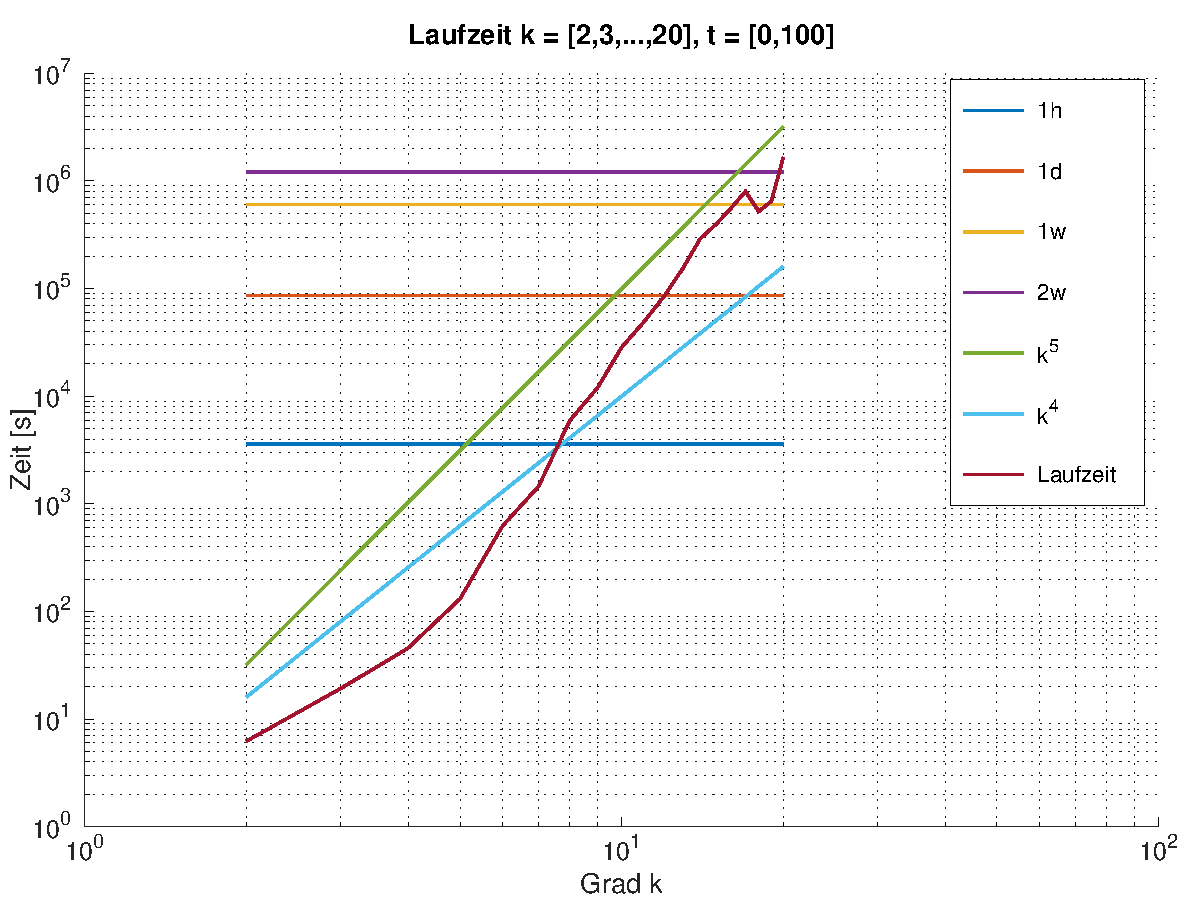
\includegraphics[width=0.49\linewidth]{lorenz2/03-images/timing_100}
	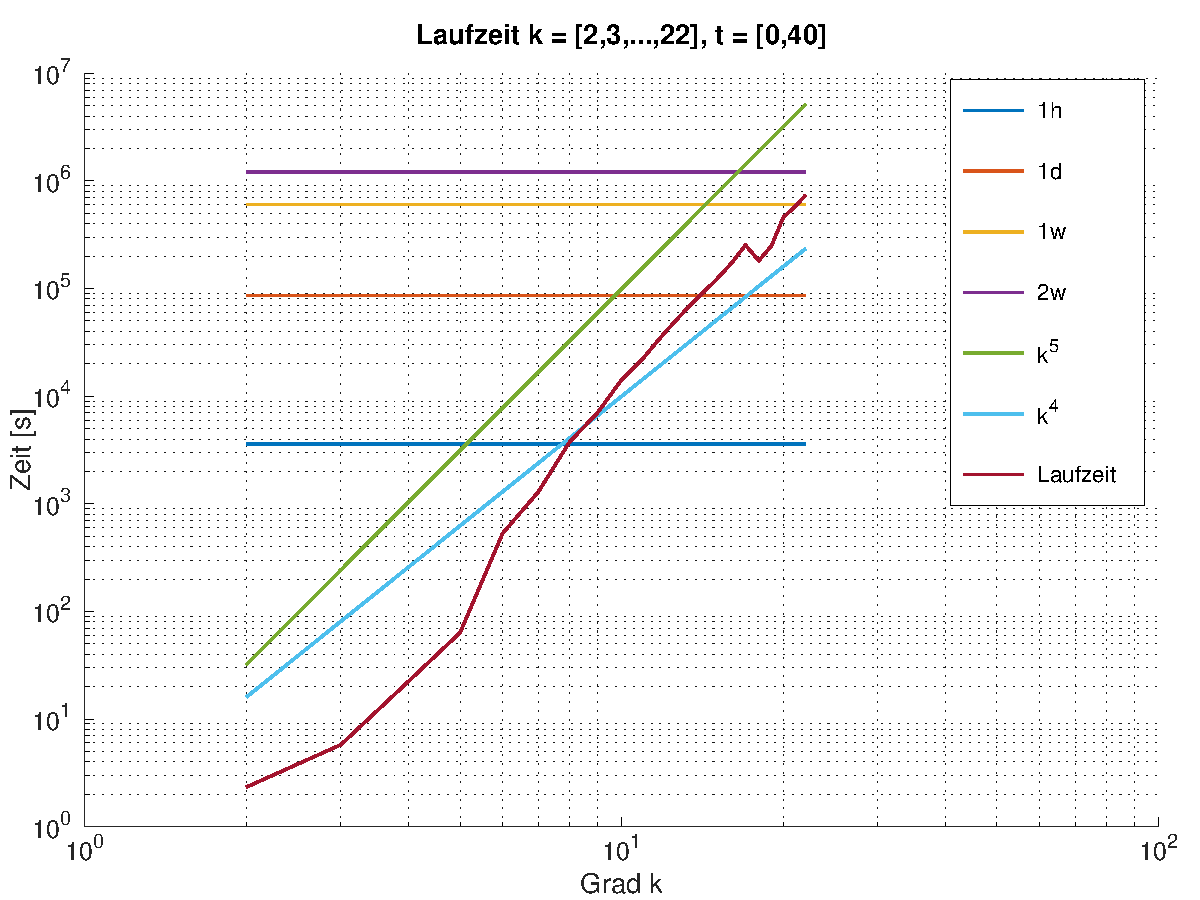
\includegraphics[width=0.49\linewidth]{lorenz2/03-images/timing_40}
	\caption{Laufzeit f"ur Berechnung von eines Lorenzsystems mit Grad $k$}
	\label{figure:lorenz2:timings}
\end{figure}

\begin{figure}
	\centering
	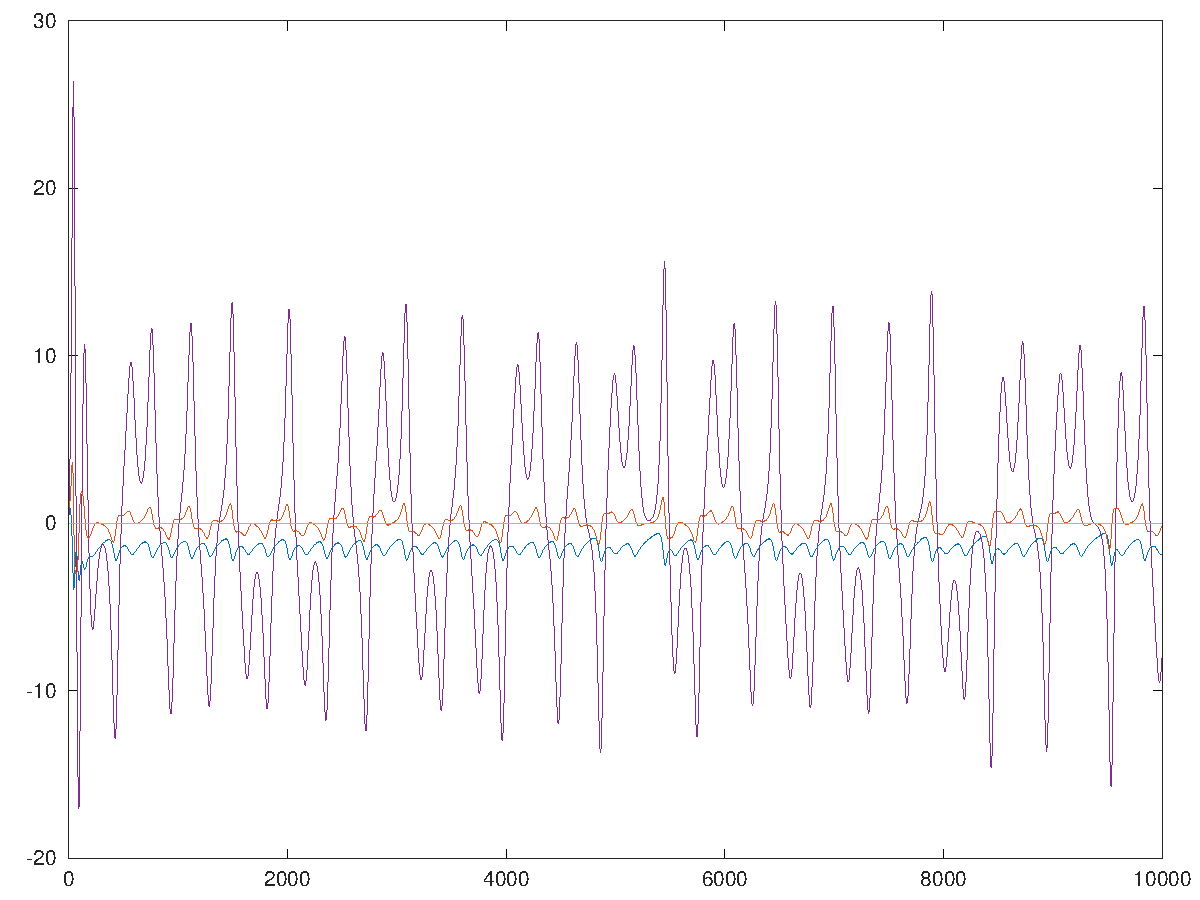
\includegraphics[width=0.49\linewidth]{{lorenz2/03-images/ord2.X}.pdf}
	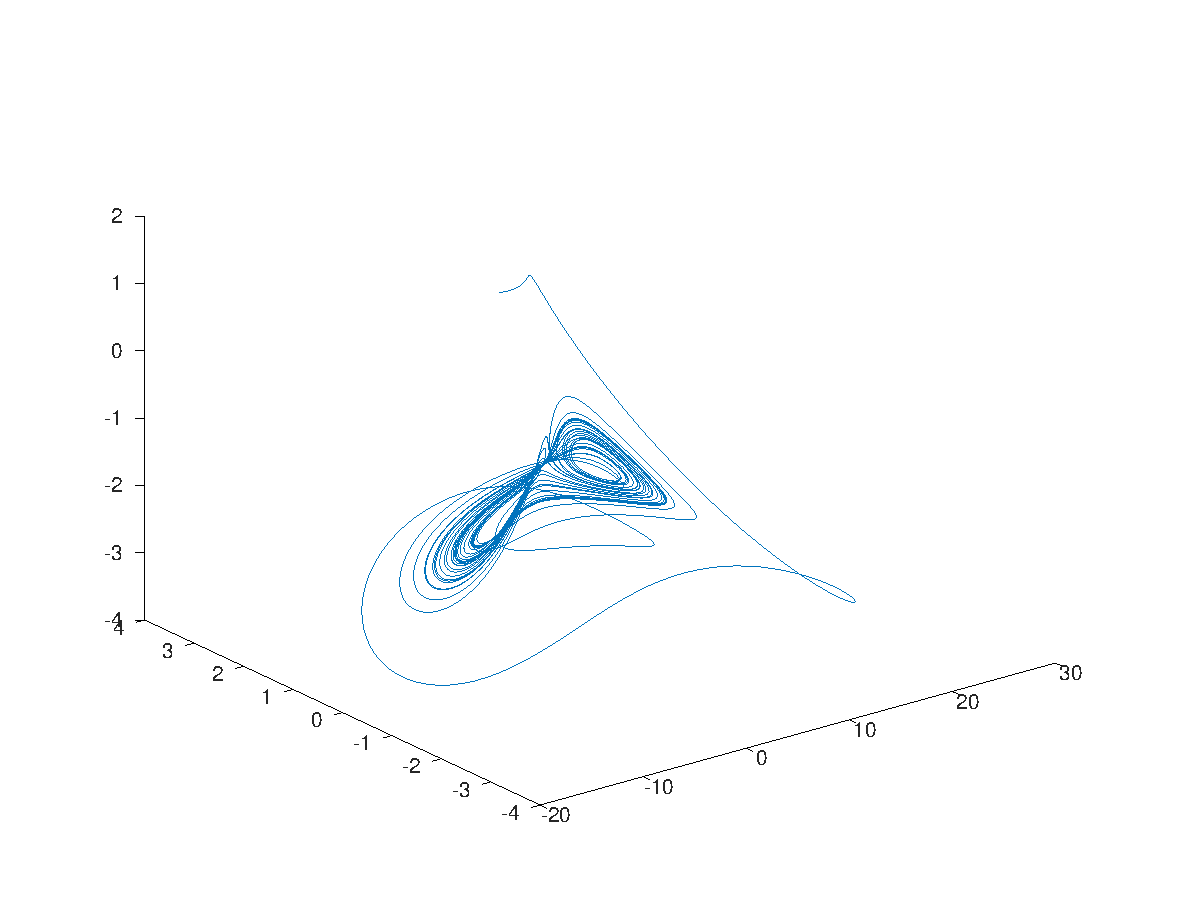
\includegraphics[width=0.49\linewidth]{{lorenz2/03-images/ord2.butterfly}.pdf}
	\caption{Lorenzssystem mit Grad 2}
	\label{figure:lorenz2:systemdeg2}
\end{figure}

\begin{figure}
	\centering
	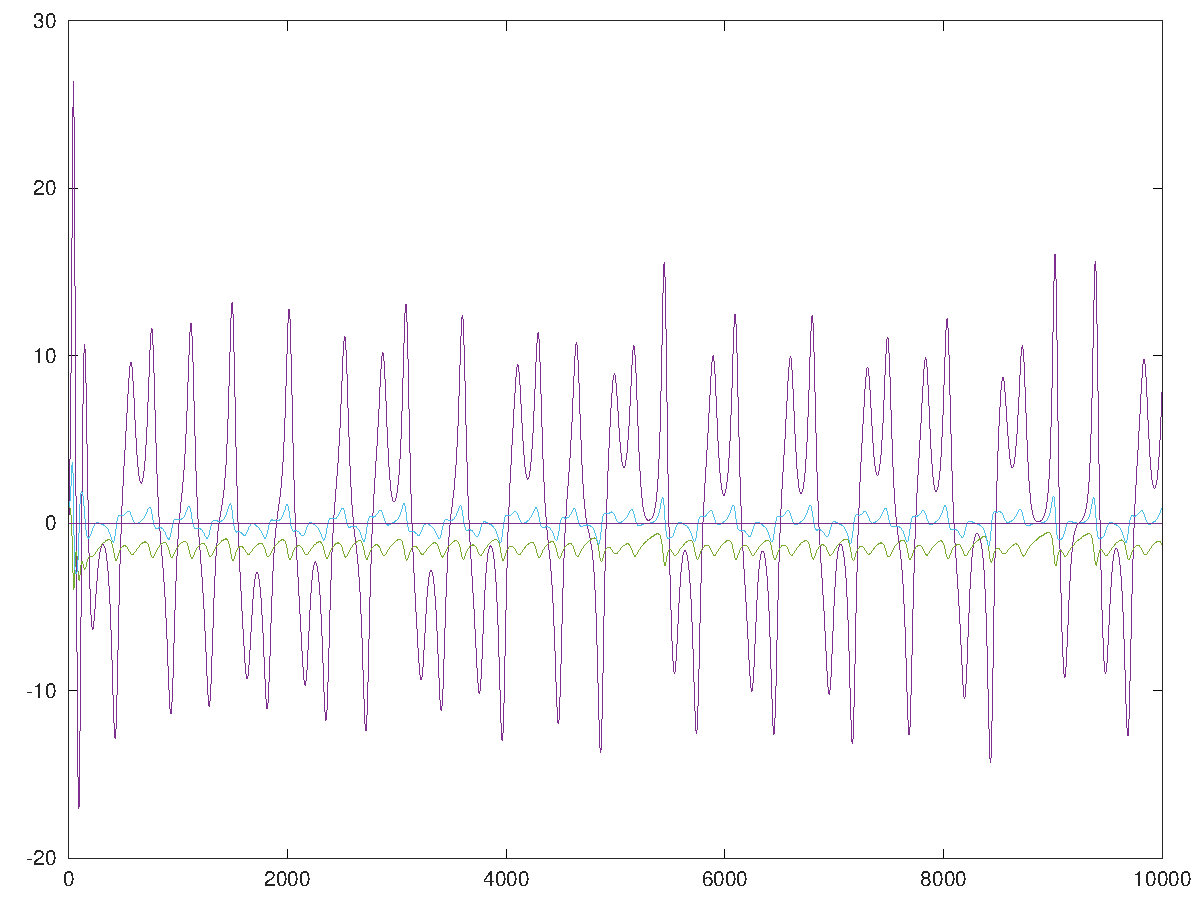
\includegraphics[width=0.49\linewidth]{{lorenz2/03-images/ord3.X}.pdf}
	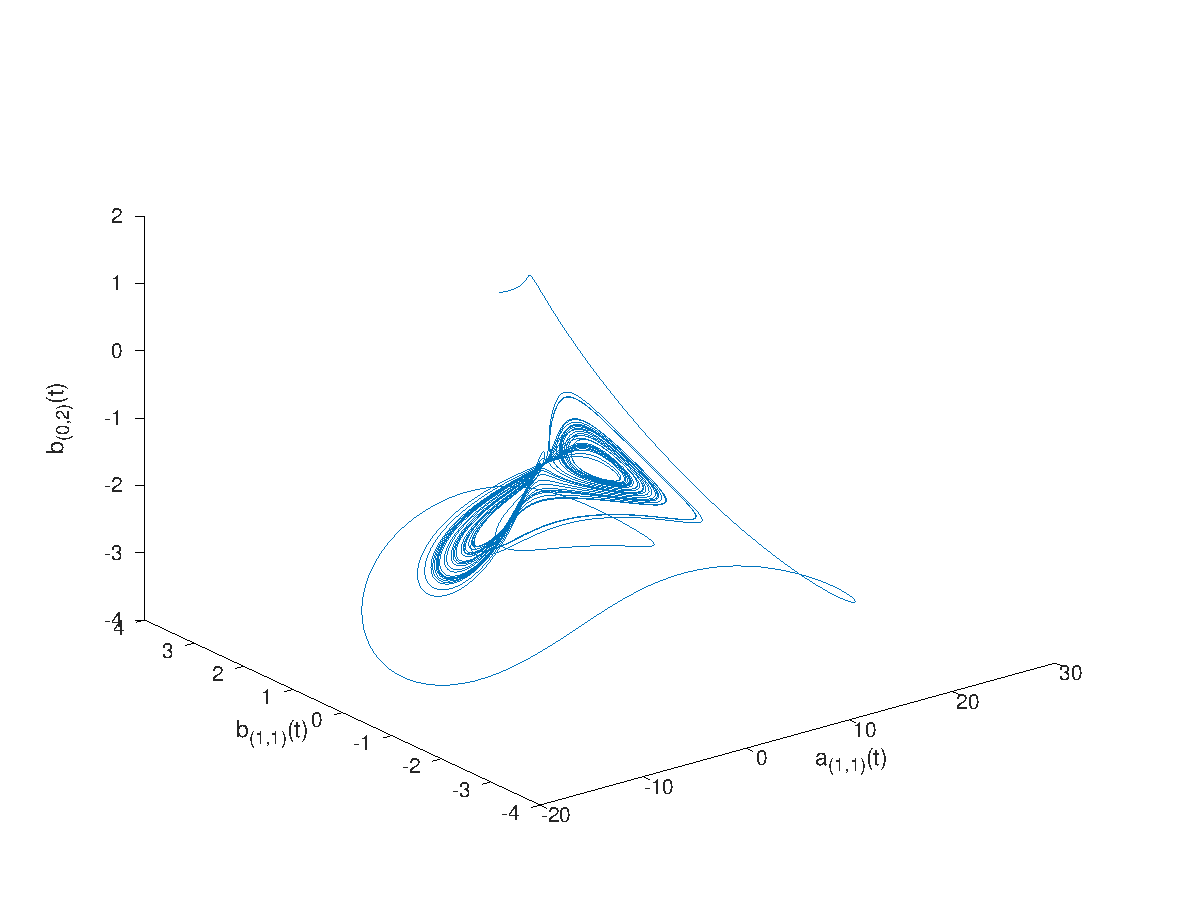
\includegraphics[width=0.49\linewidth]{{lorenz2/03-images/ord3.butterfly}.pdf}
	\caption{Lorenzssystem mit Grad 3}
	\label{figure:lorenz2:systemdeg3}
\end{figure}

\begin{figure}
	\centering
	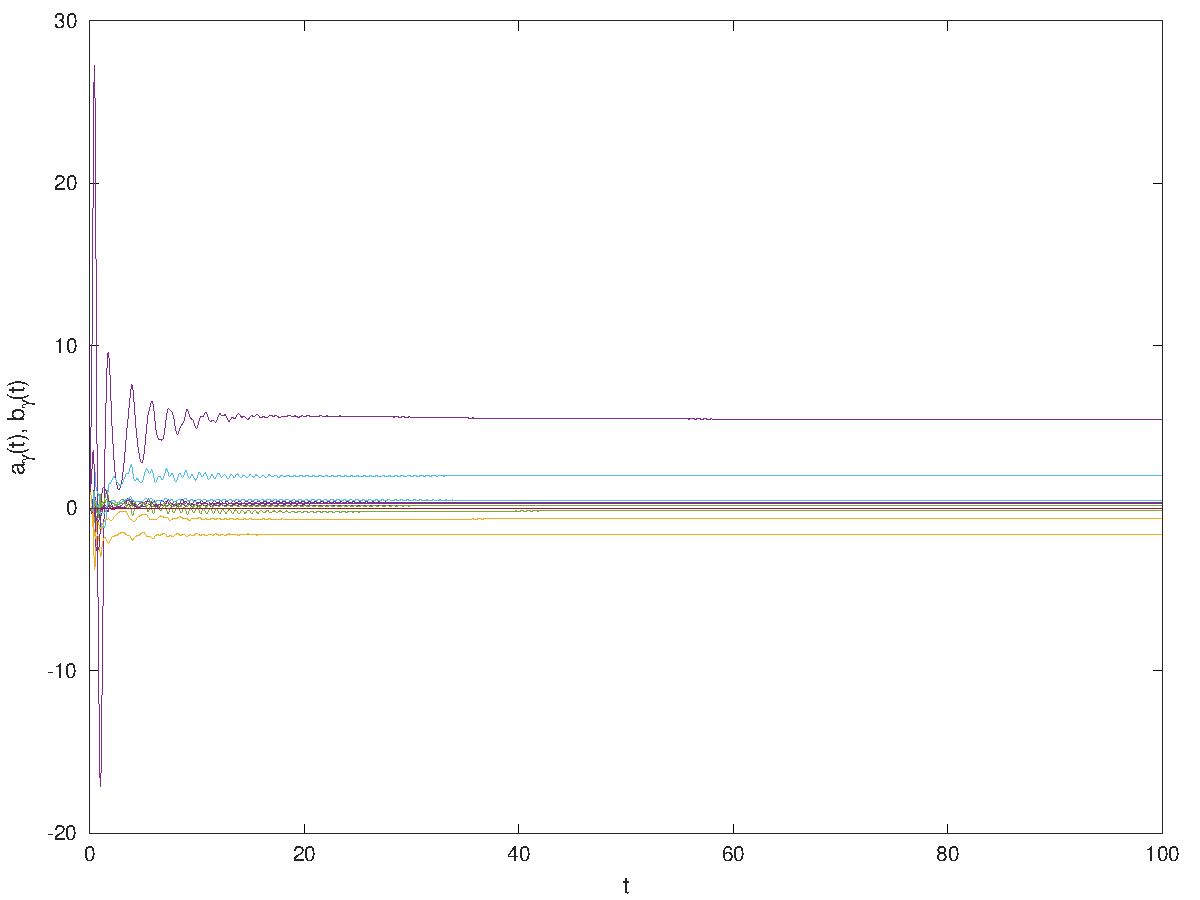
\includegraphics[width=0.49\linewidth]{{lorenz2/03-images/ord4.X}.pdf}
	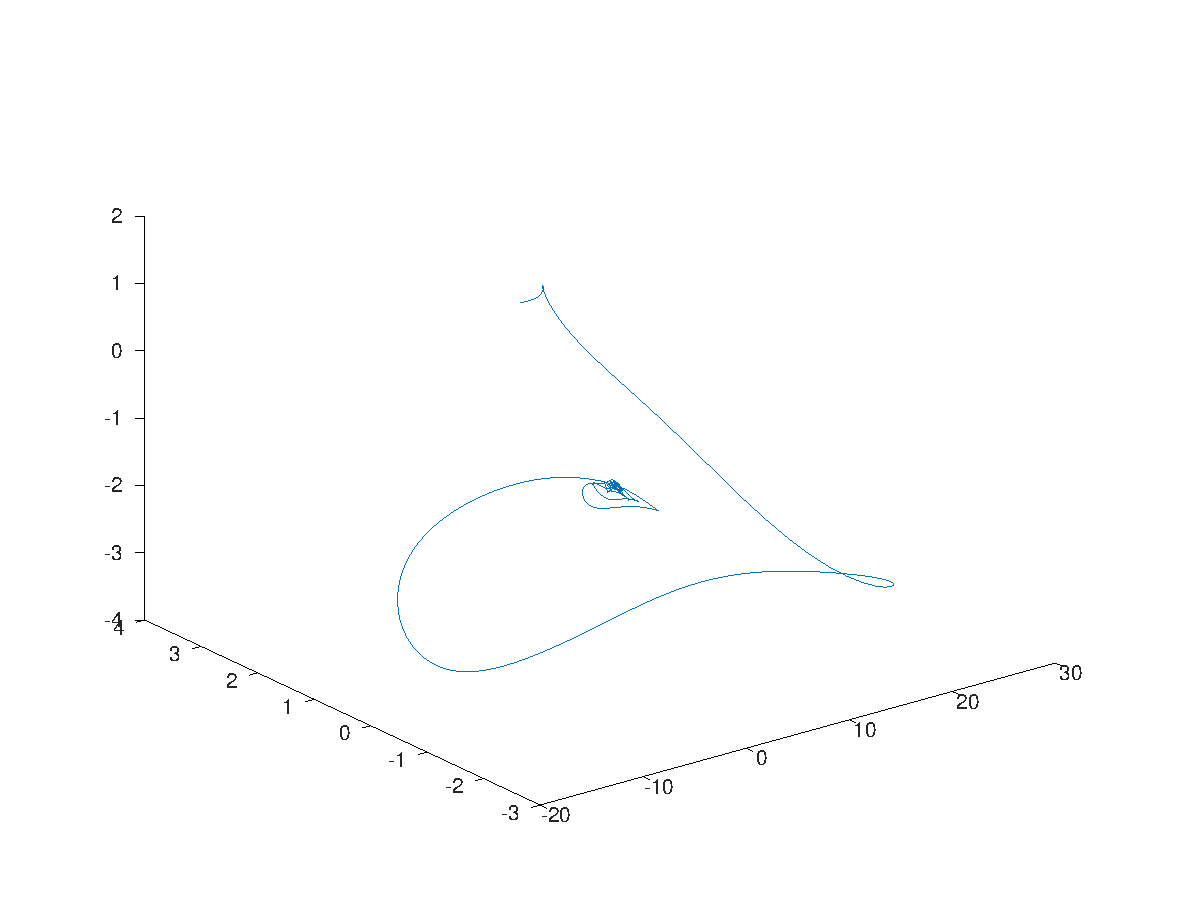
\includegraphics[width=0.49\linewidth]{{lorenz2/03-images/ord4.butterfly}.pdf}
	\caption{Lorenzssystem mit Grad 4}
	\label{figure:lorenz2:systemdeg4}
\end{figure}

\begin{figure}
	\centering
	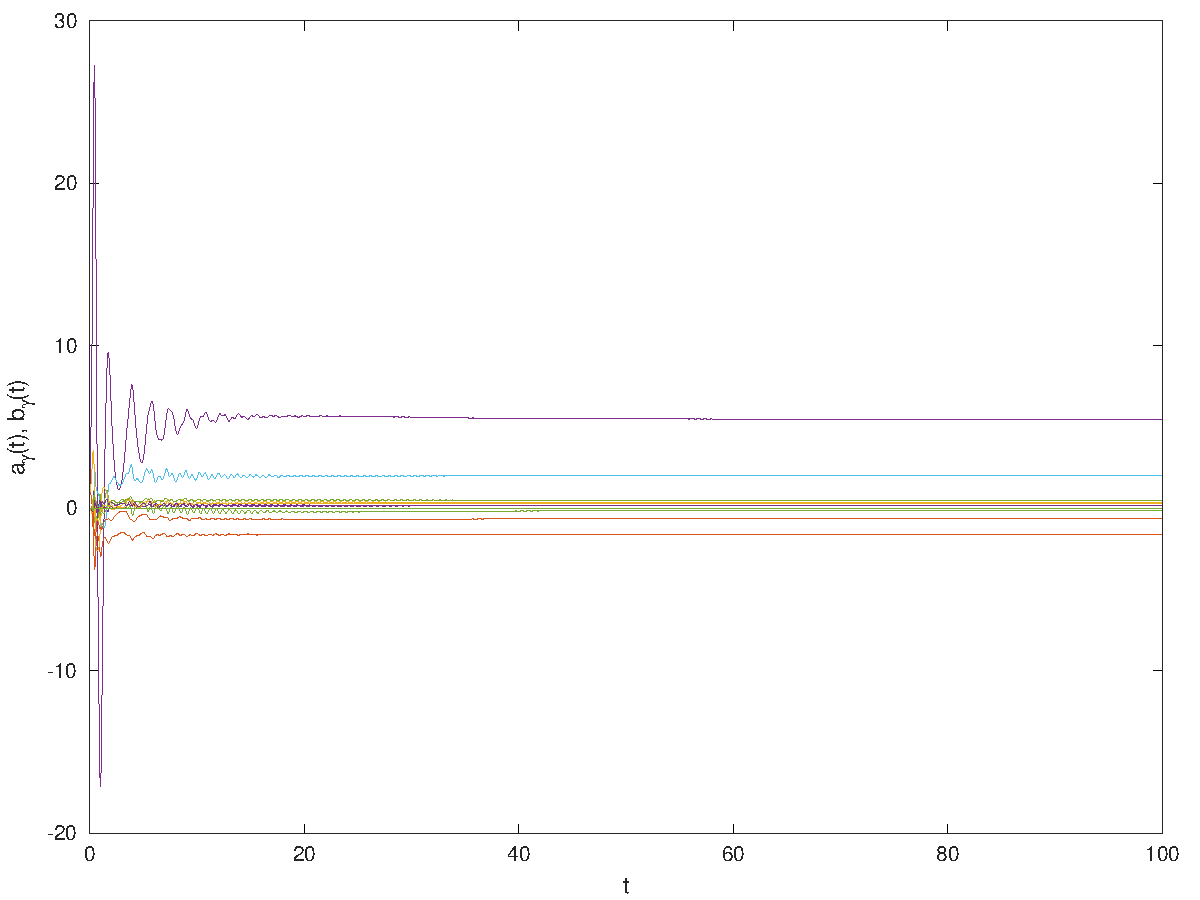
\includegraphics[width=0.49\linewidth]{{lorenz2/03-images/ord5.X}.pdf}
	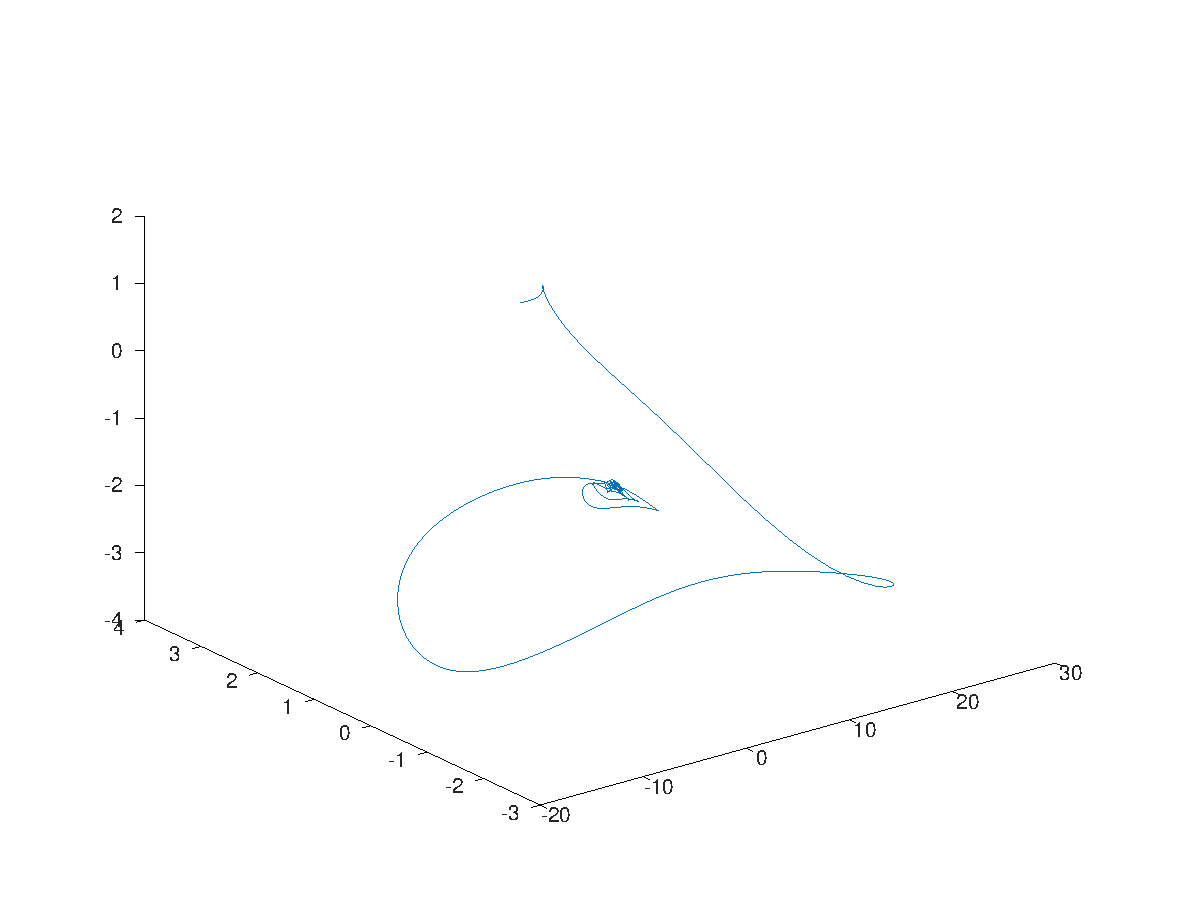
\includegraphics[width=0.49\linewidth]{{lorenz2/03-images/ord5.butterfly}.pdf}
	\caption{Lorenzssystem mit Grad 5}
	\label{figure:lorenz2:systemdeg5}
\end{figure}

\begin{figure}
	\centering
	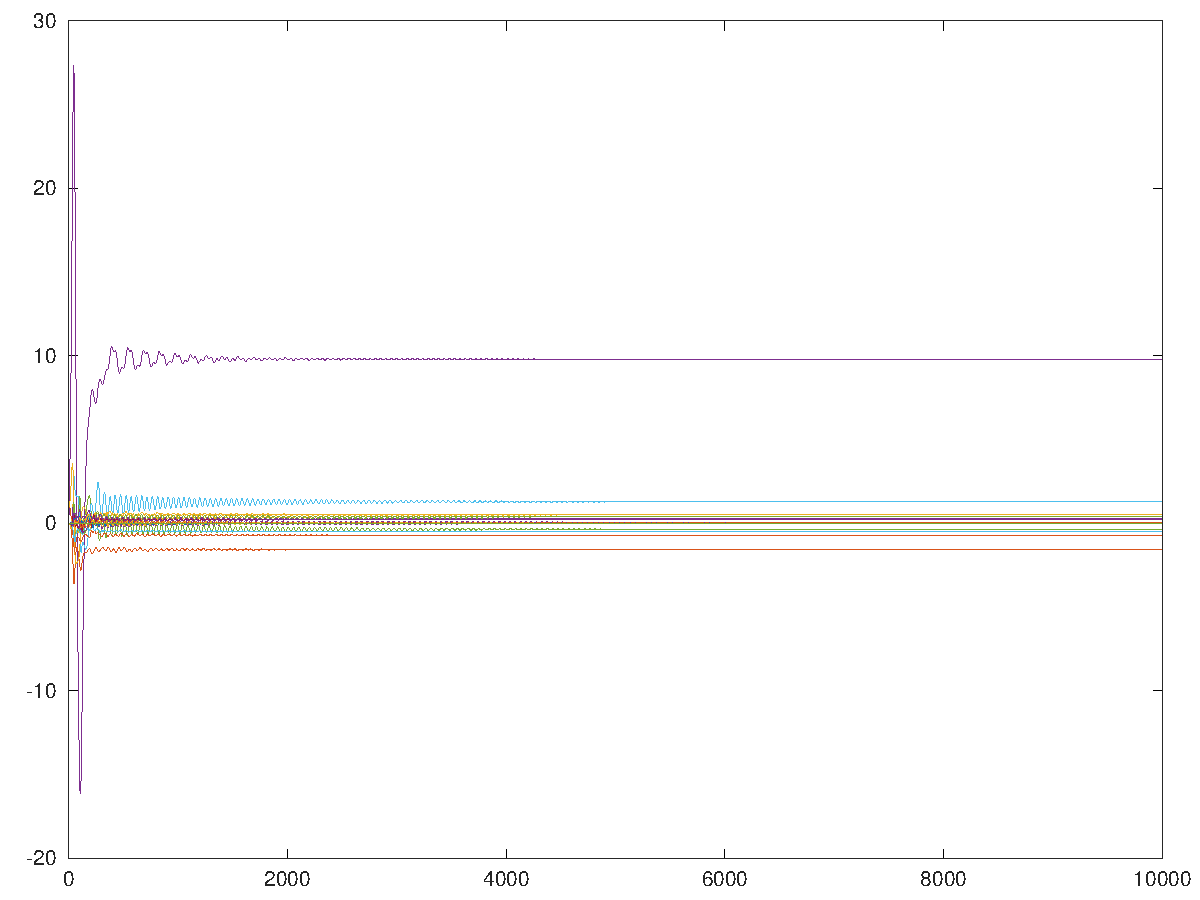
\includegraphics[width=0.49\linewidth]{{lorenz2/03-images/ord6.X}.pdf}
	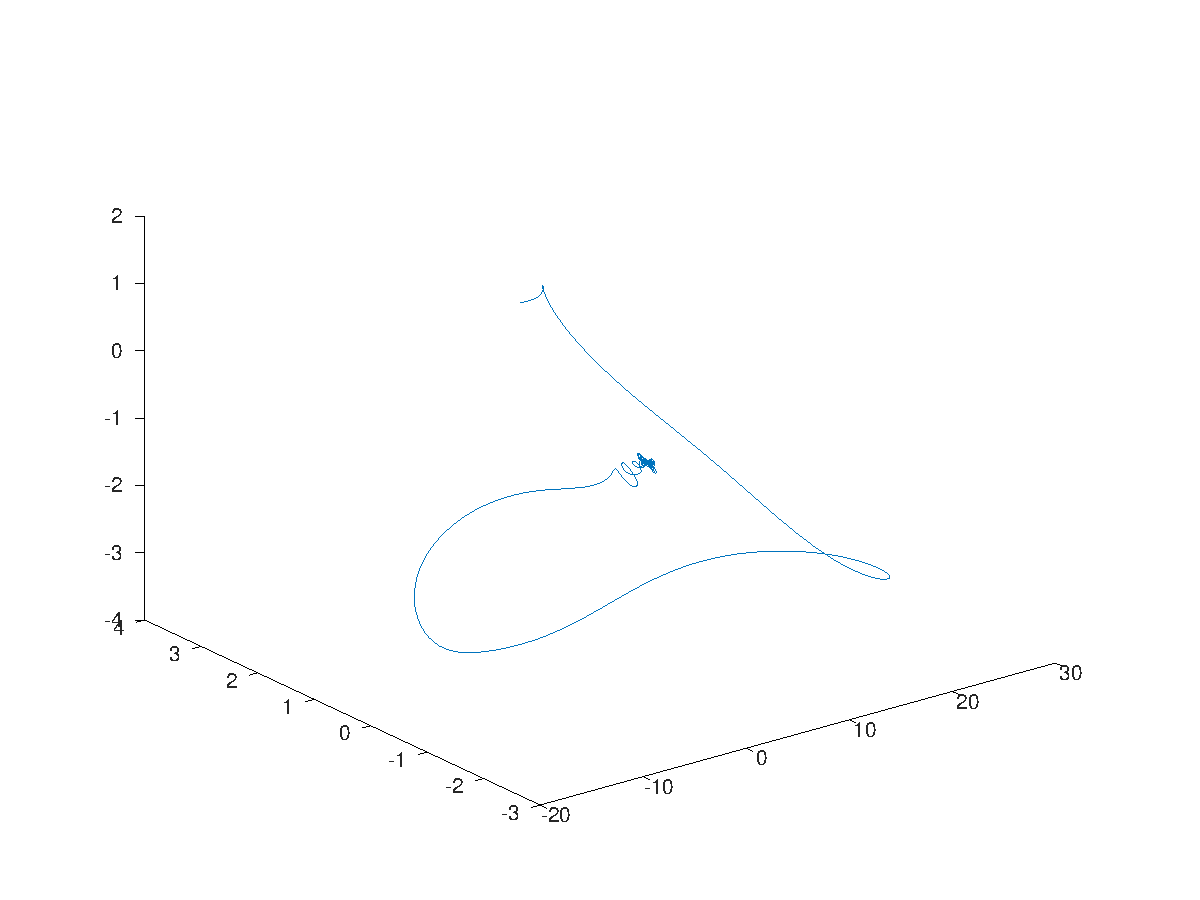
\includegraphics[width=0.49\linewidth]{{lorenz2/03-images/ord6.butterfly}.pdf}
	\caption{Lorenzssystem mit Grad 6}
	\label{figure:lorenz2:systemdeg6}
\end{figure}

\begin{figure}
	\centering
	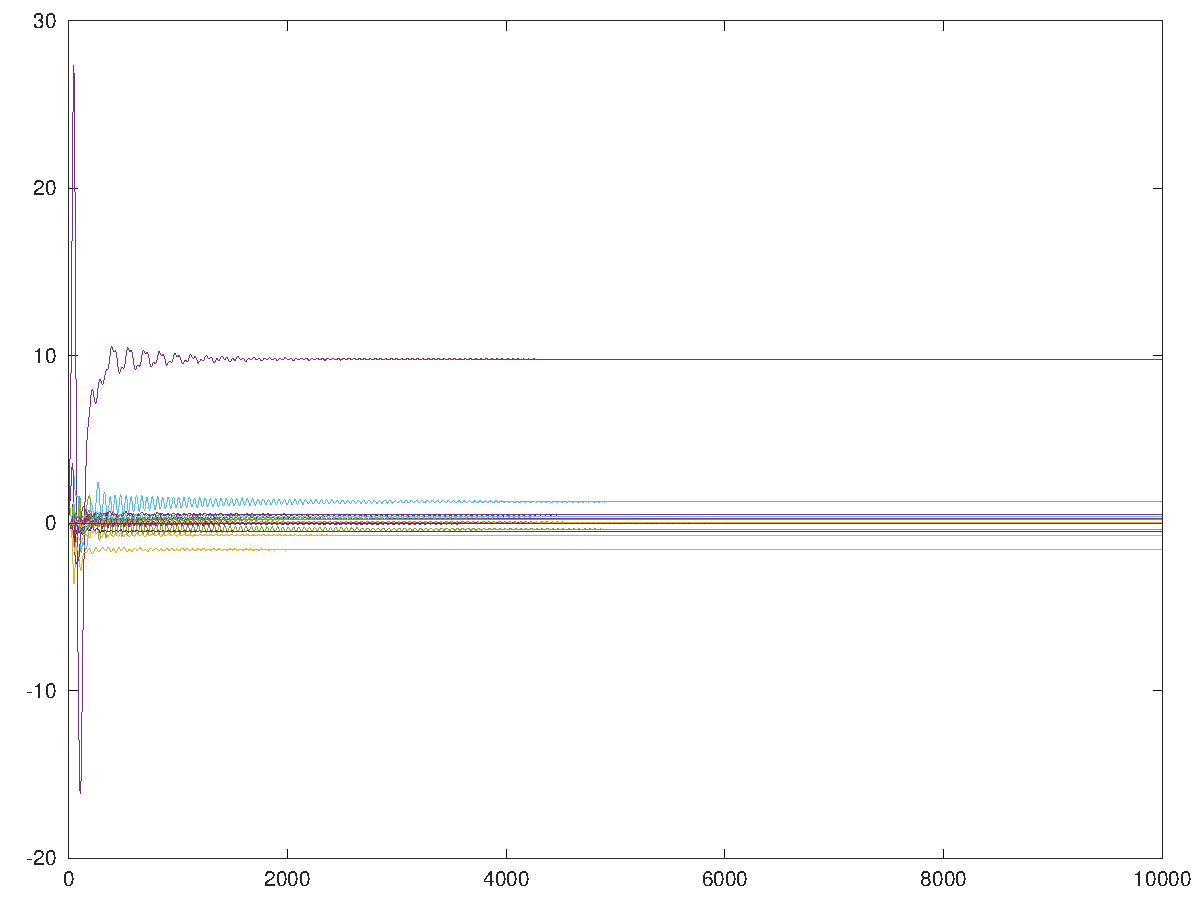
\includegraphics[width=0.49\linewidth]{{lorenz2/03-images/ord7.X}.pdf}
	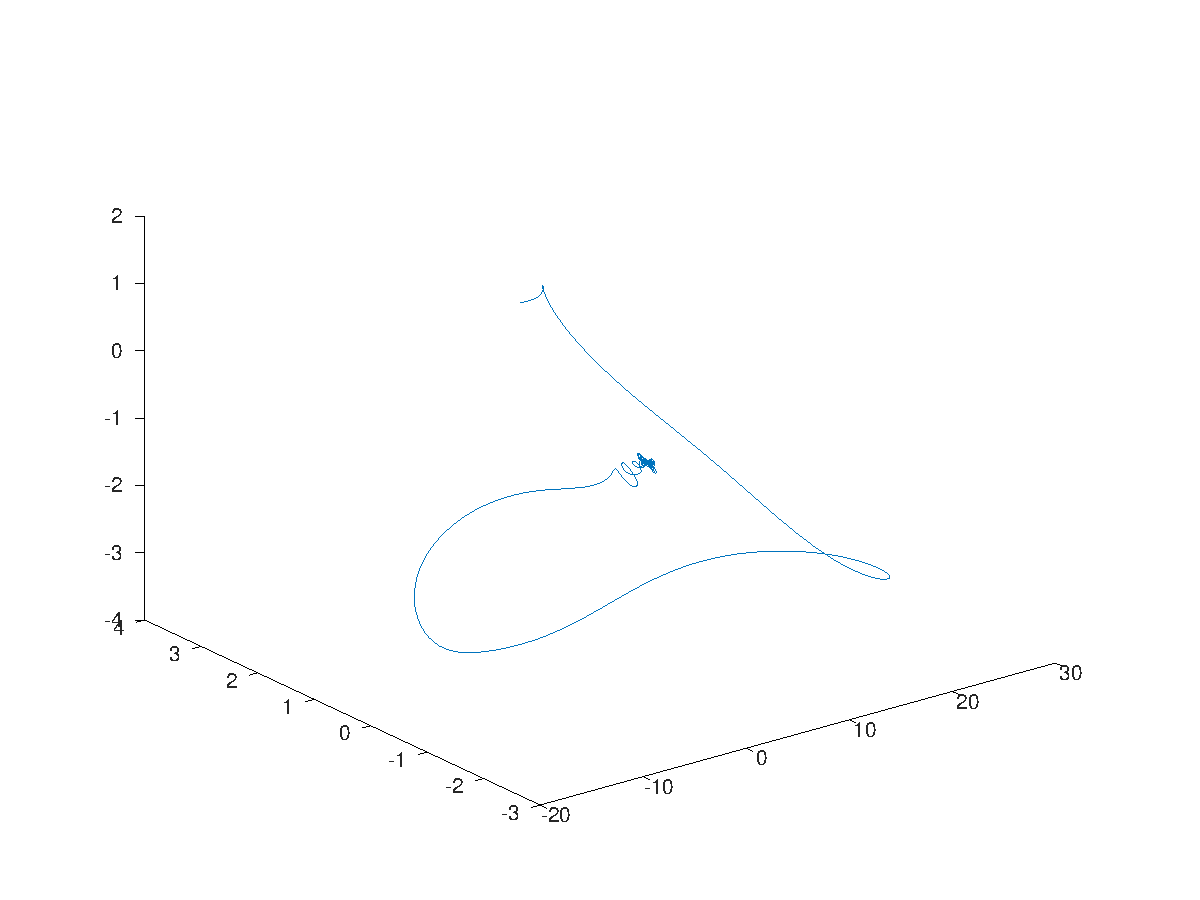
\includegraphics[width=0.49\linewidth]{{lorenz2/03-images/ord7.butterfly}.pdf}
	\caption{Lorenzssystem mit Grad 7}
	\label{figure:lorenz2:systemdeg7}
\end{figure}

\begin{figure}
	\centering
	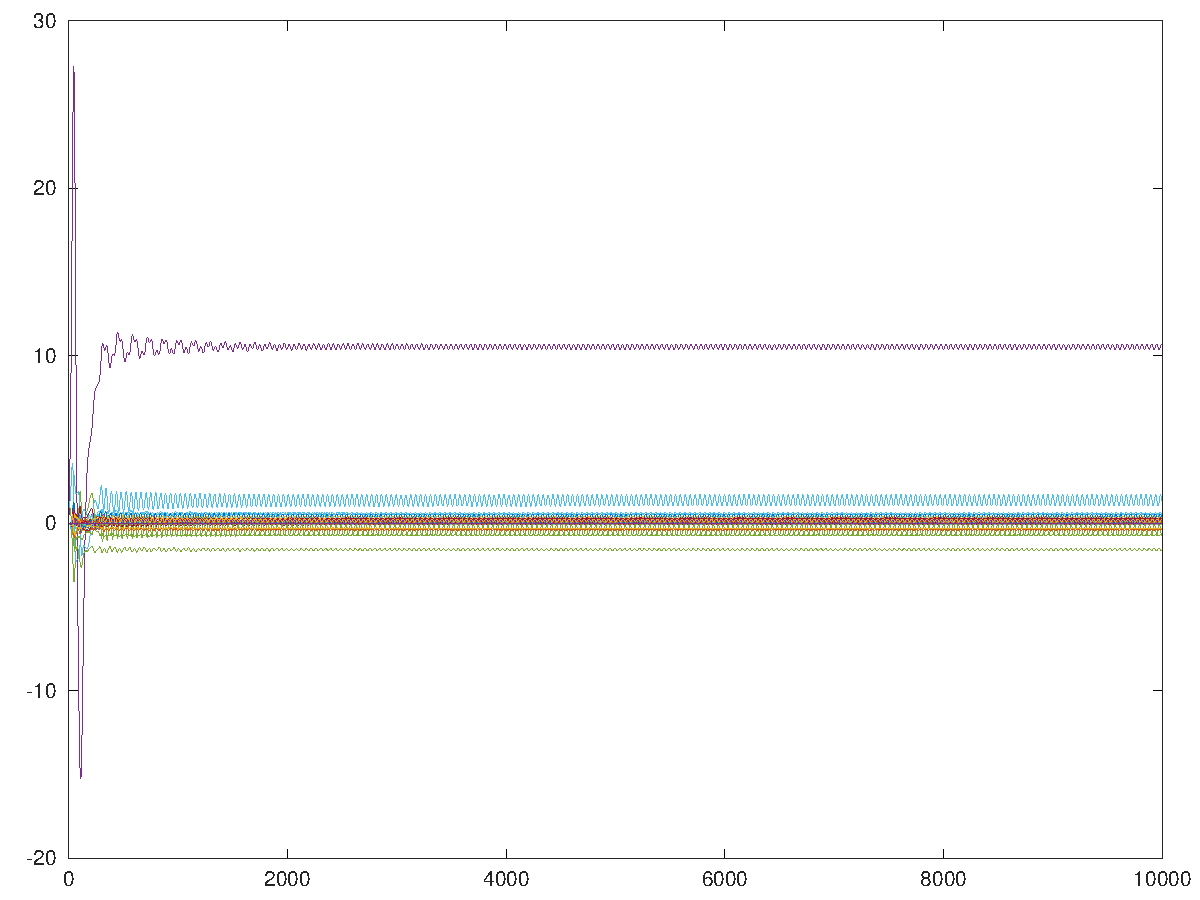
\includegraphics[width=0.49\linewidth]{{lorenz2/03-images/ord8.X}.pdf}
	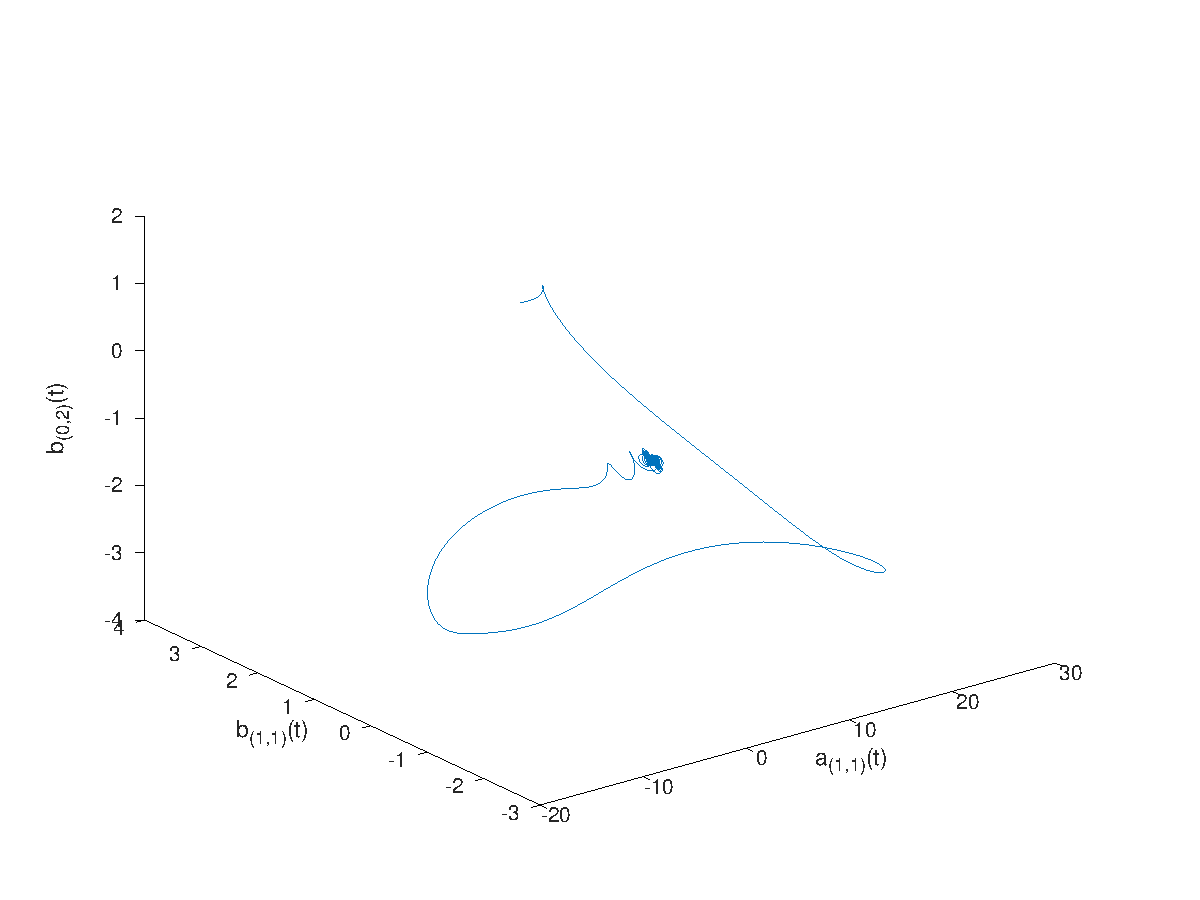
\includegraphics[width=0.49\linewidth]{{lorenz2/03-images/ord8.butterfly}.pdf}
	\caption{Lorenzssystem mit Grad 8}
	\label{figure:lorenz2:systemdeg8}
\end{figure}

\begin{figure}
	\centering
	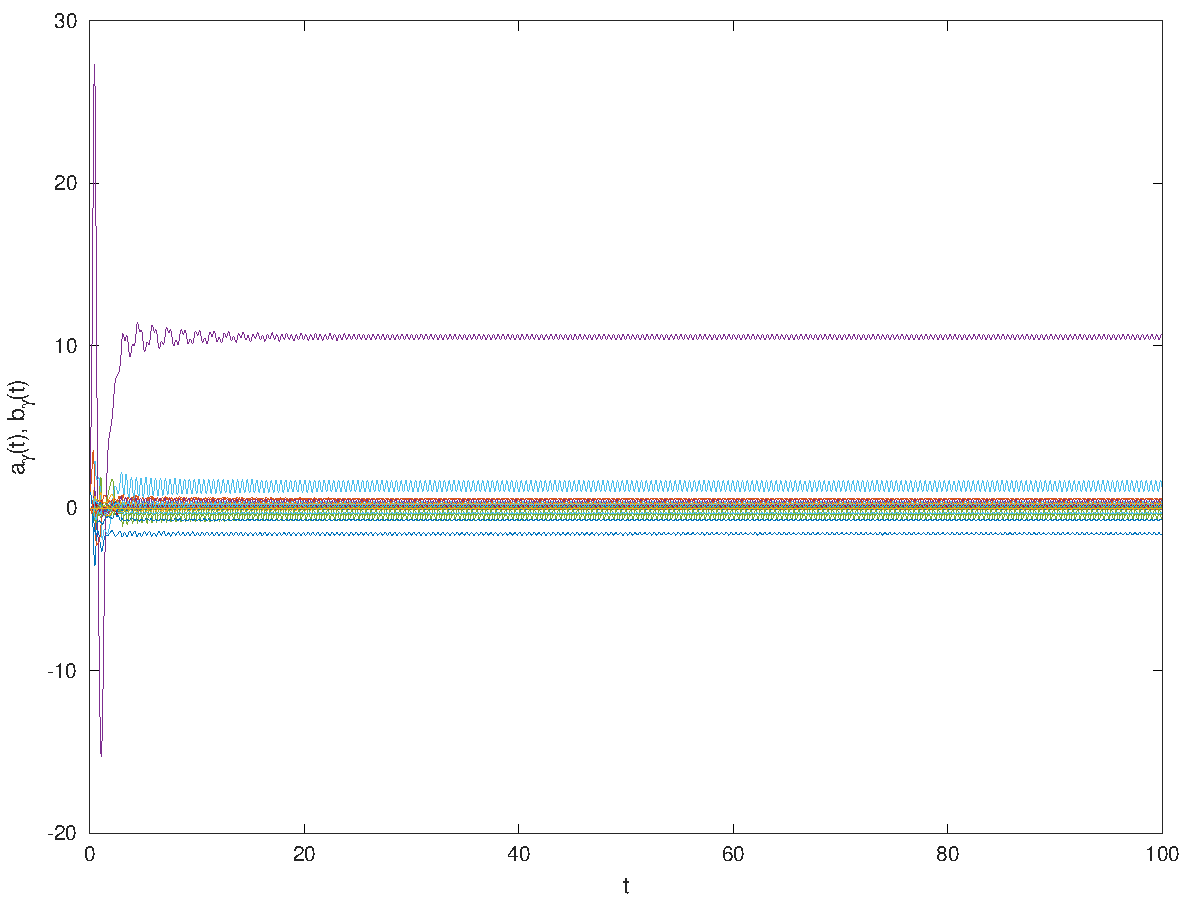
\includegraphics[width=0.49\linewidth]{{lorenz2/03-images/ord9.X}.pdf}
	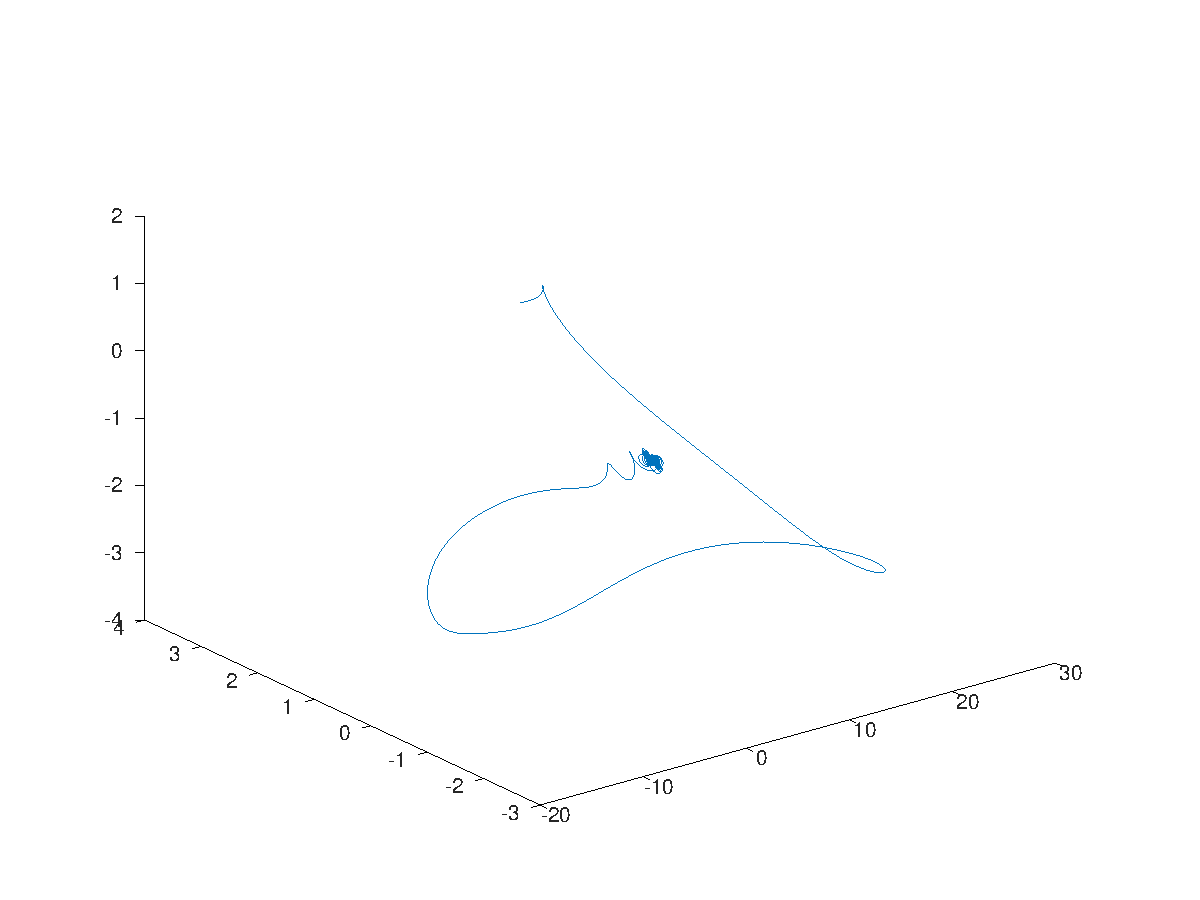
\includegraphics[width=0.49\linewidth]{{lorenz2/03-images/ord9.butterfly}.pdf}
	\caption{Lorenzssystem mit Grad 9}
	\label{figure:lorenz2:systemdeg9}
\end{figure}

\begin{figure}
	\centering
	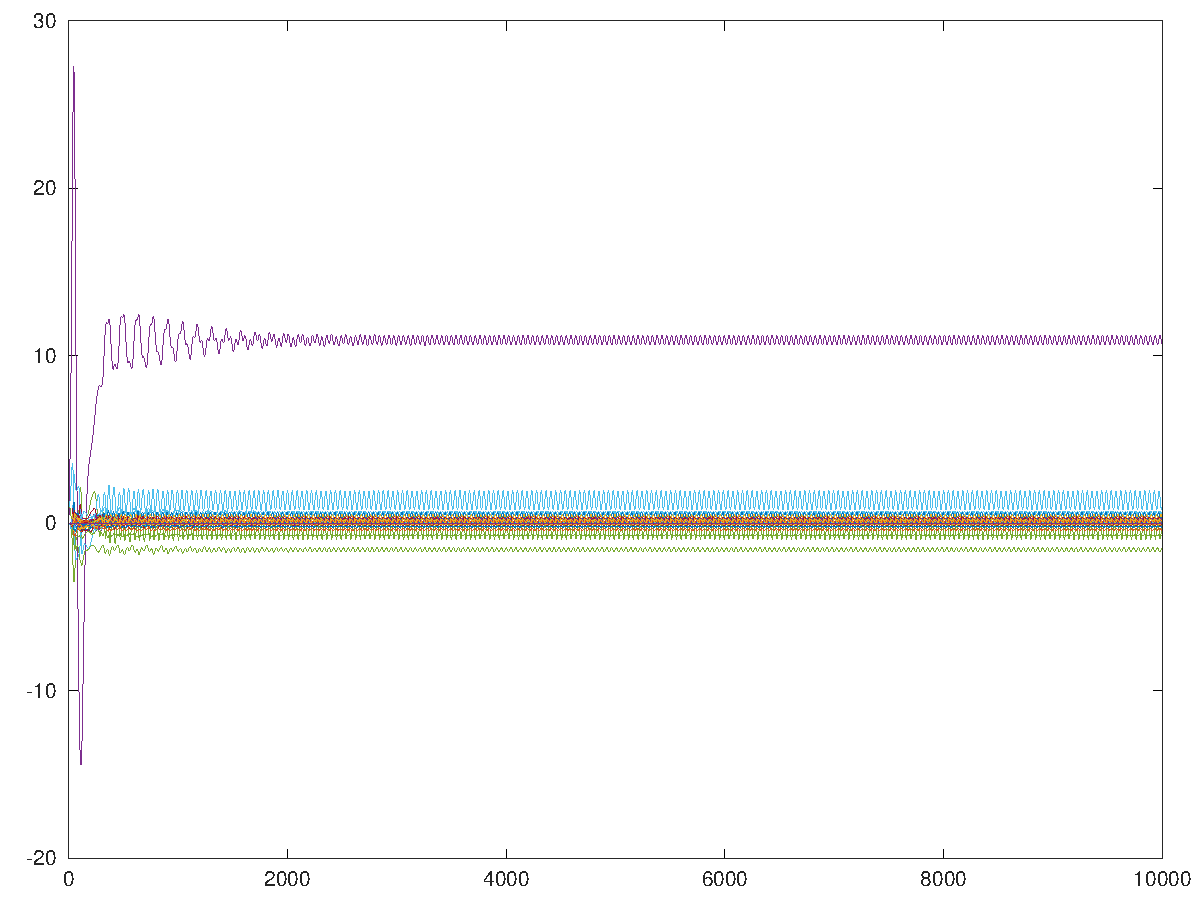
\includegraphics[width=0.49\linewidth]{{lorenz2/03-images/ord10.X}.pdf}
	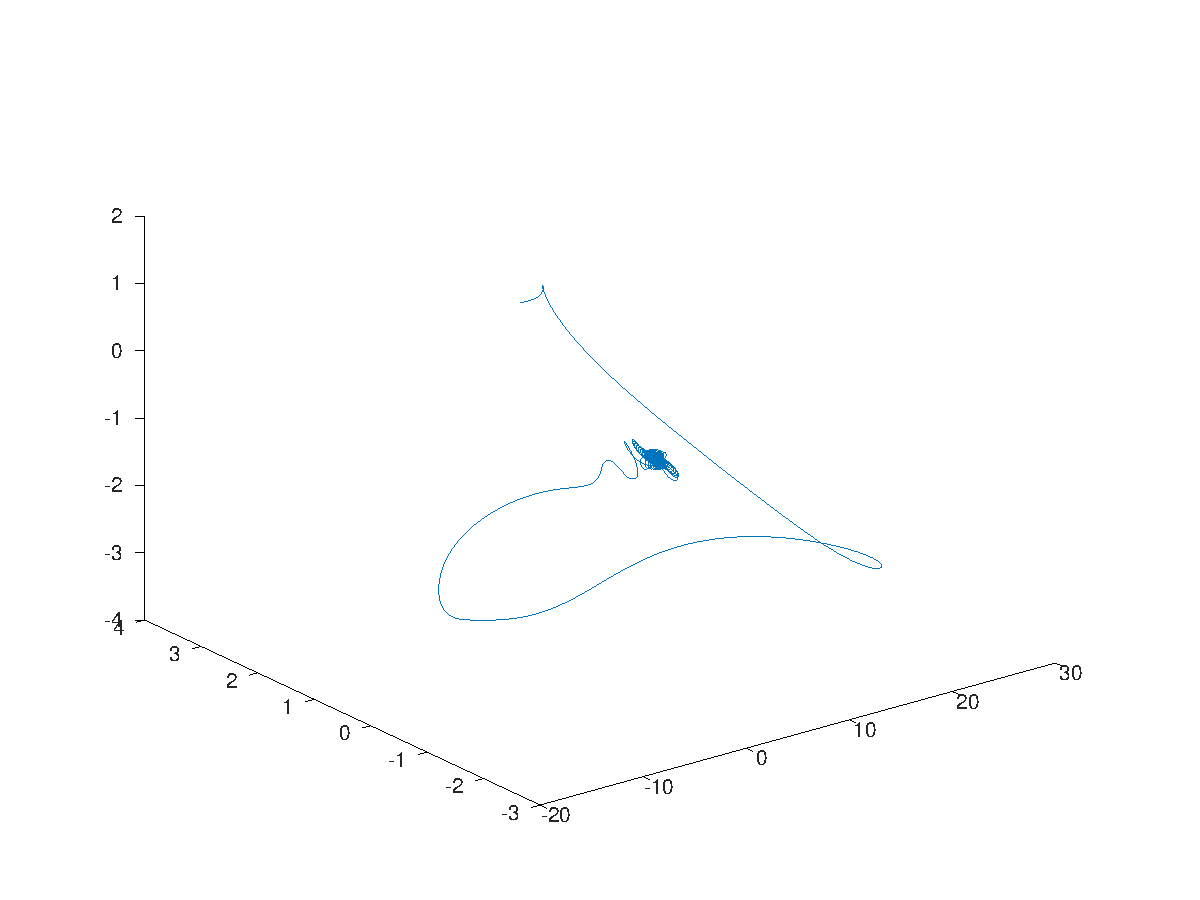
\includegraphics[width=0.49\linewidth]{{lorenz2/03-images/ord10.butterfly}.pdf}
	\caption{Lorenzssystem mit Grad 10, $t = [0,100]$}
	\label{figure:lorenz2:systemdeg10}
\end{figure}

\begin{figure}
	\centering
	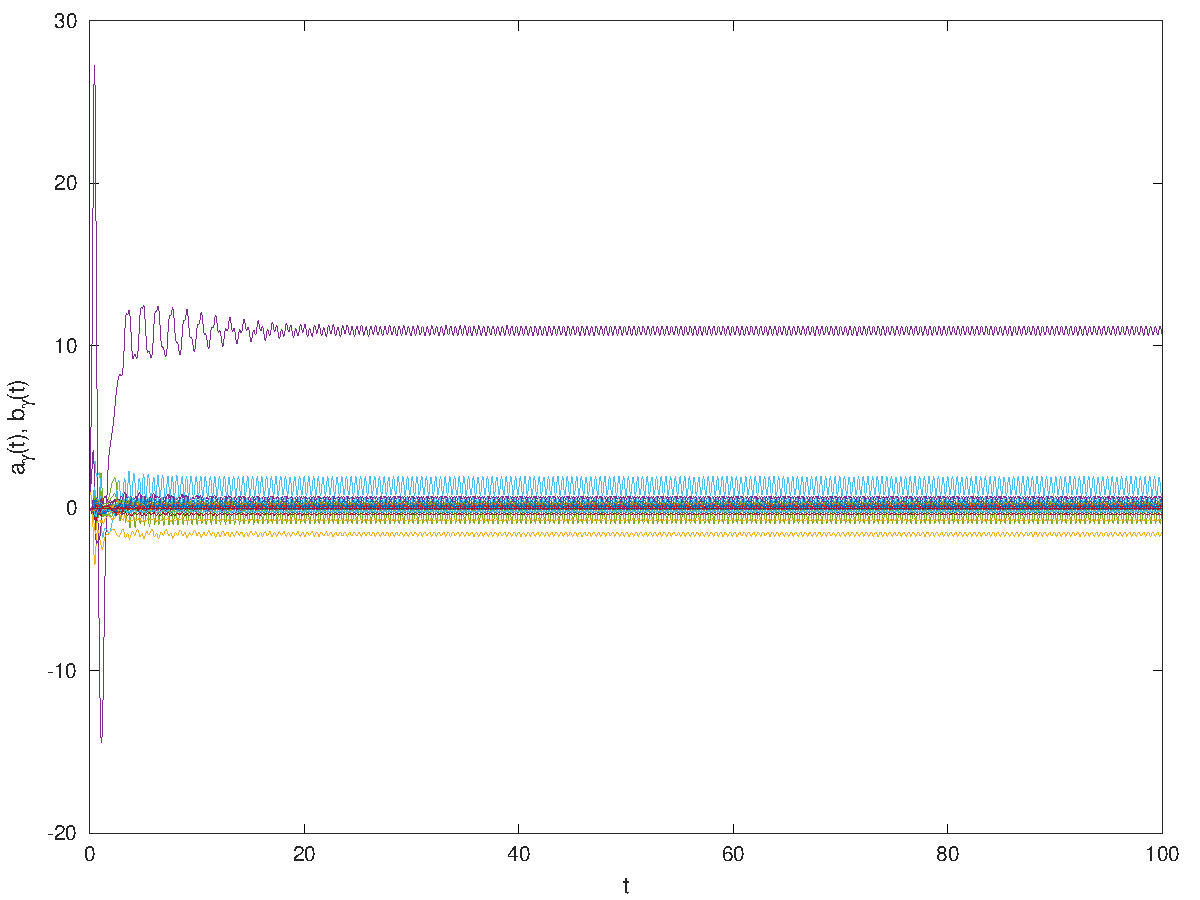
\includegraphics[width=0.49\linewidth]{{lorenz2/03-images/ord11.X}.pdf}
	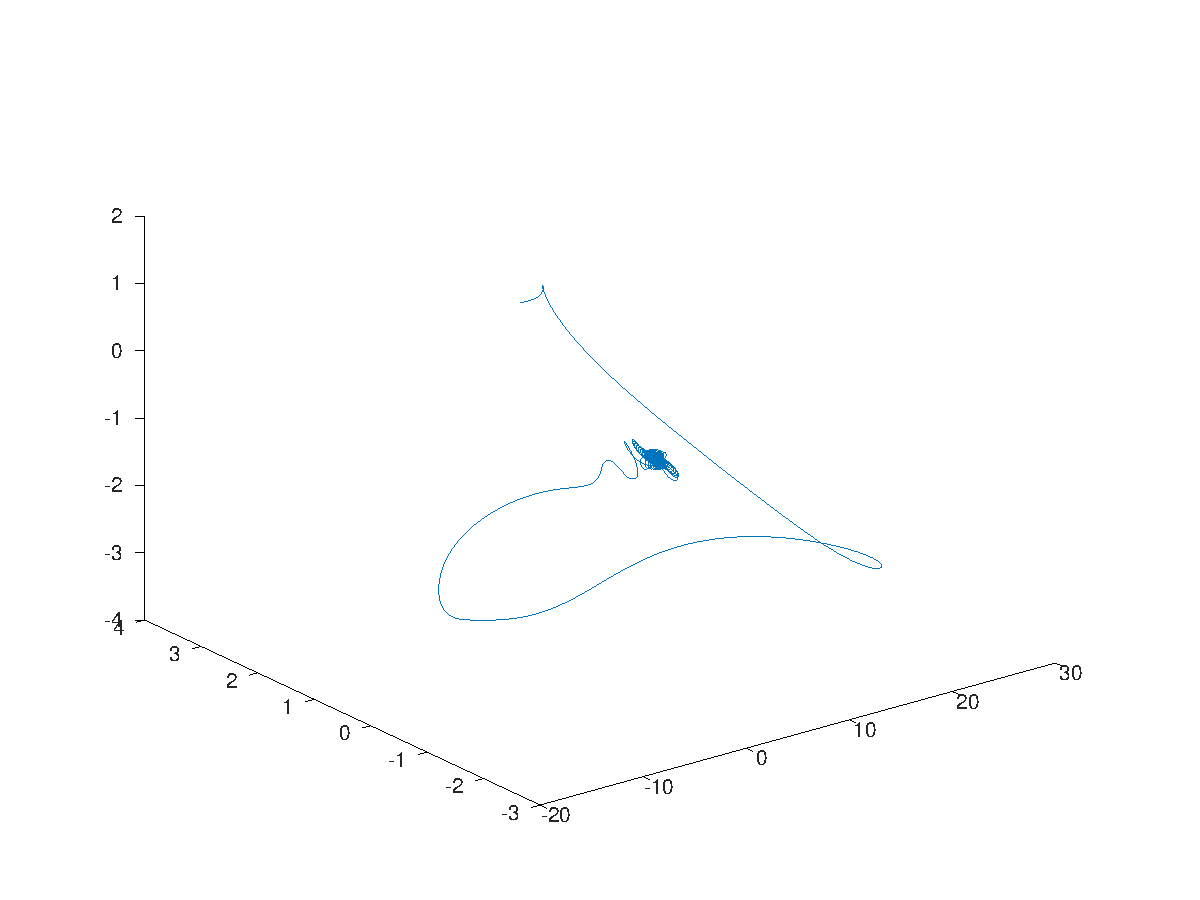
\includegraphics[width=0.49\linewidth]{{lorenz2/03-images/ord11.butterfly}.pdf}
	\caption{Lorenzssystem mit Grad 11, $t = [0,100]$}
	\label{figure:lorenz2:systemdeg11}
\end{figure}

\begin{figure}
	\centering
	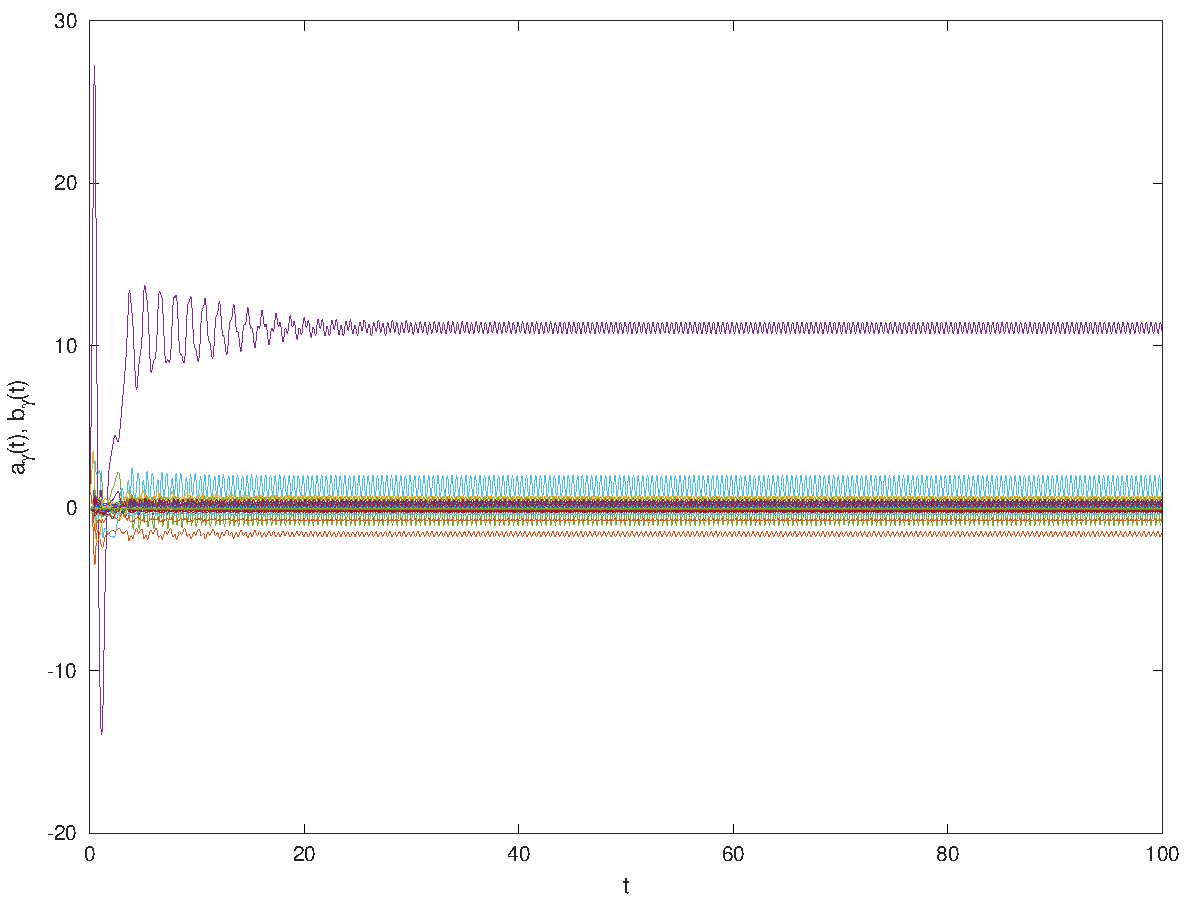
\includegraphics[width=0.49\linewidth]{{lorenz2/03-images/ord12.X}.pdf}
	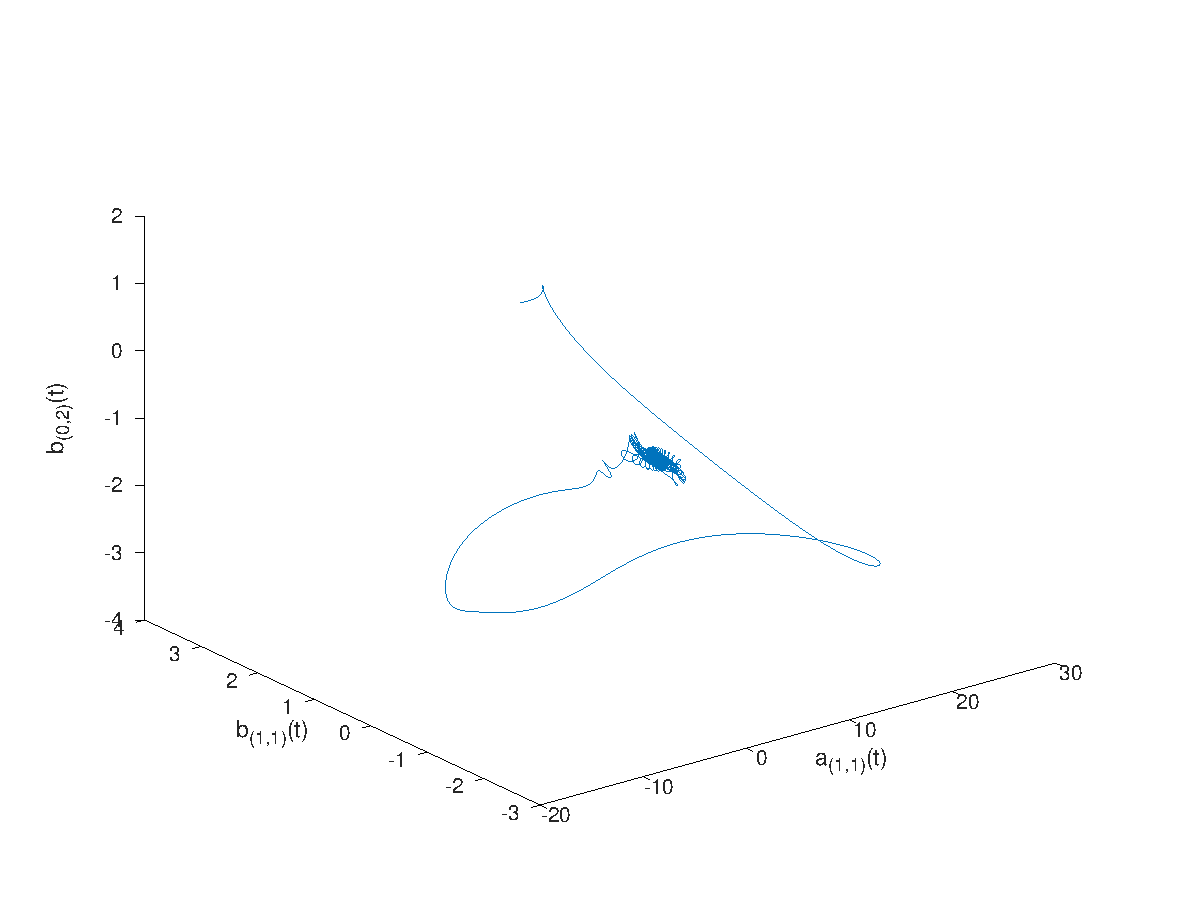
\includegraphics[width=0.49\linewidth]{{lorenz2/03-images/ord12.butterfly}.pdf}
	\caption{Lorenzssystem mit Grad 12, $t = [0,100]$}
	\label{figure:lorenz2:systemdeg12}
\end{figure}

\begin{figure}
	\centering
	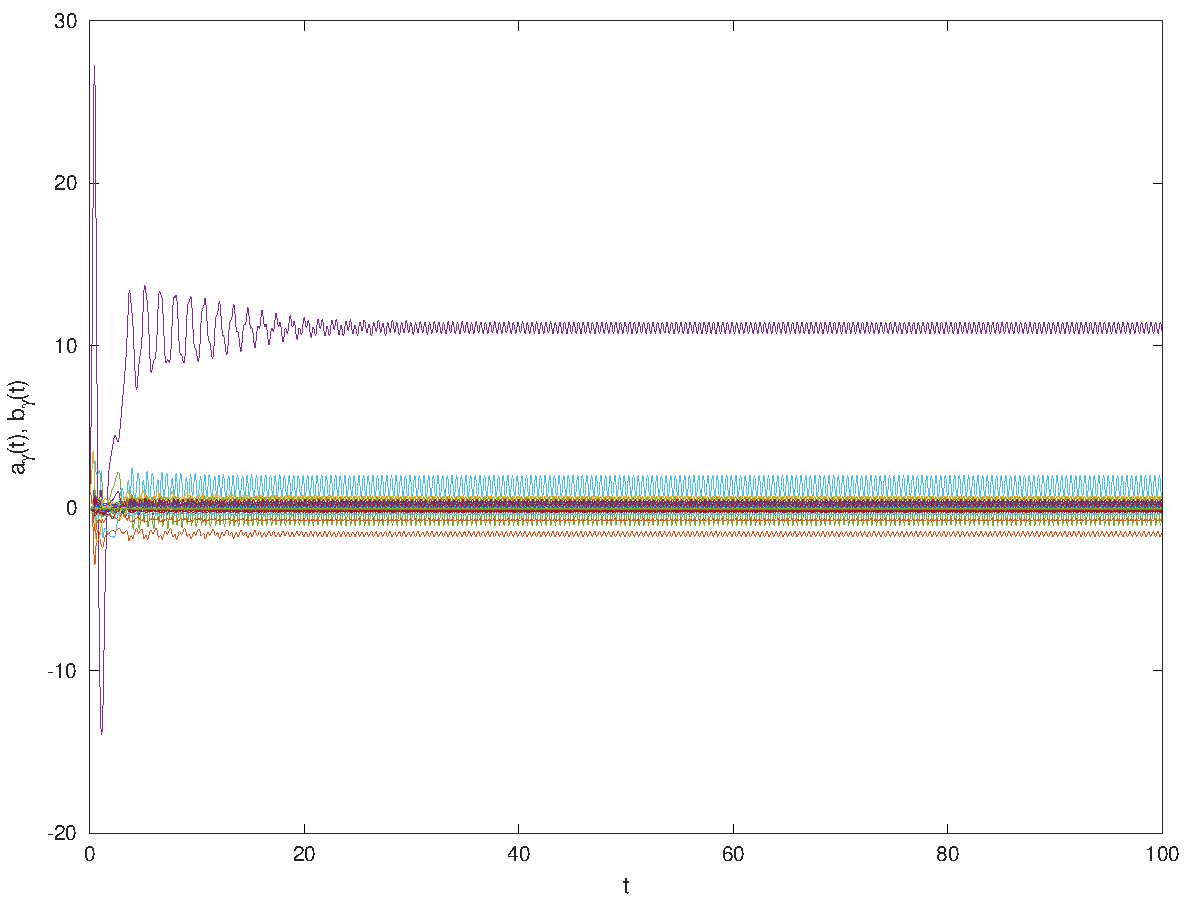
\includegraphics[width=0.49\linewidth]{{lorenz2/03-images/ord13.X}.pdf}
	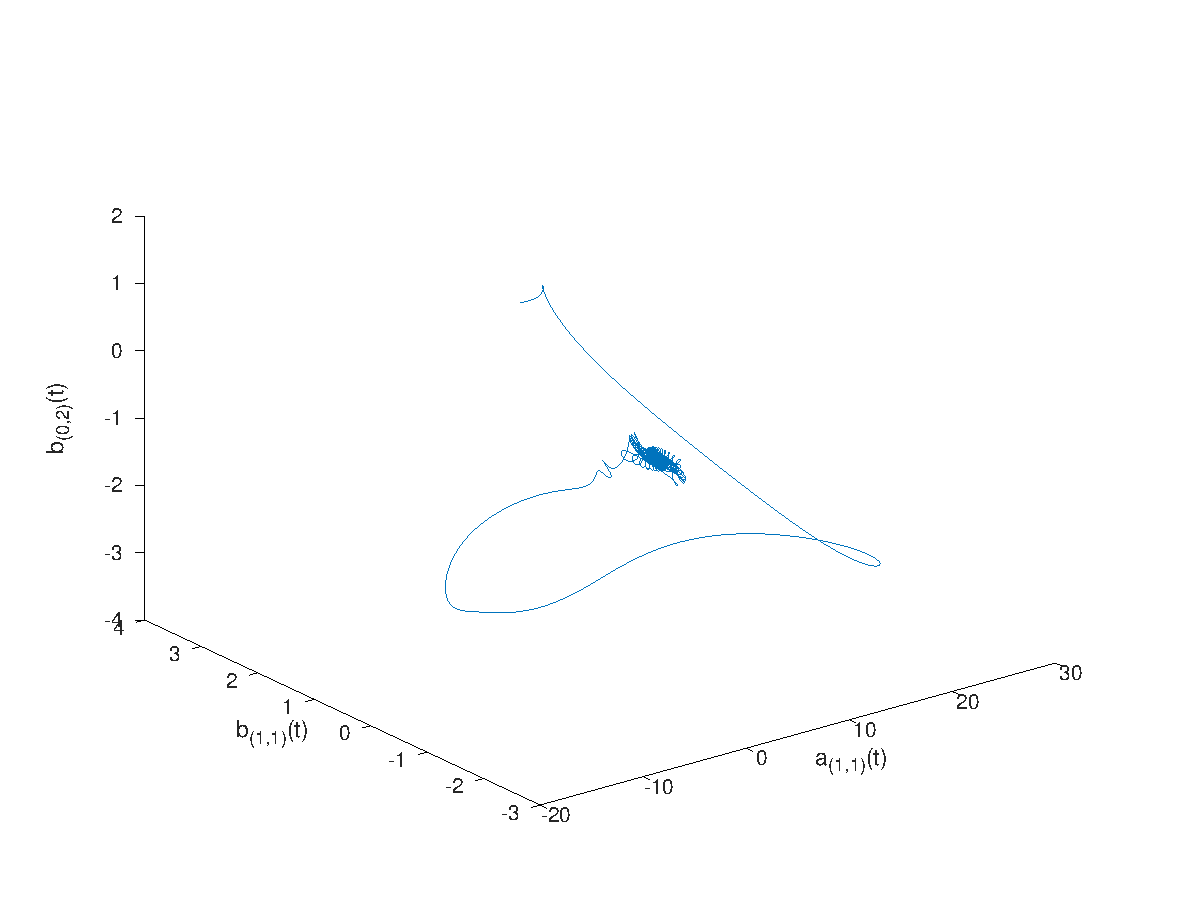
\includegraphics[width=0.49\linewidth]{{lorenz2/03-images/ord13.butterfly}.pdf}
	\caption{Lorenzssystem mit Grad 13, $t = [0,100]$}
	\label{figure:lorenz2:systemdeg13}
\end{figure}

\begin{figure}
	\centering
	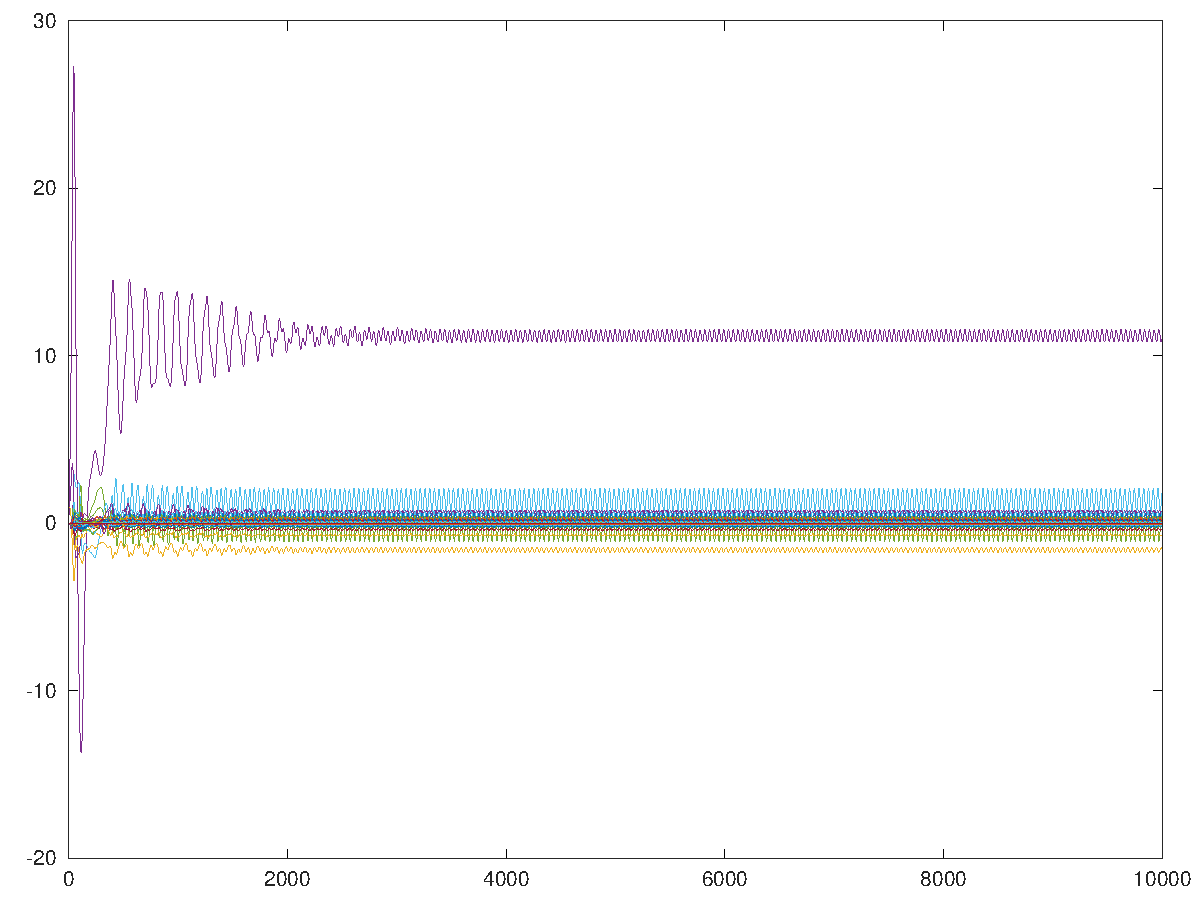
\includegraphics[width=0.49\linewidth]{{lorenz2/03-images/ord14.X}.pdf}
	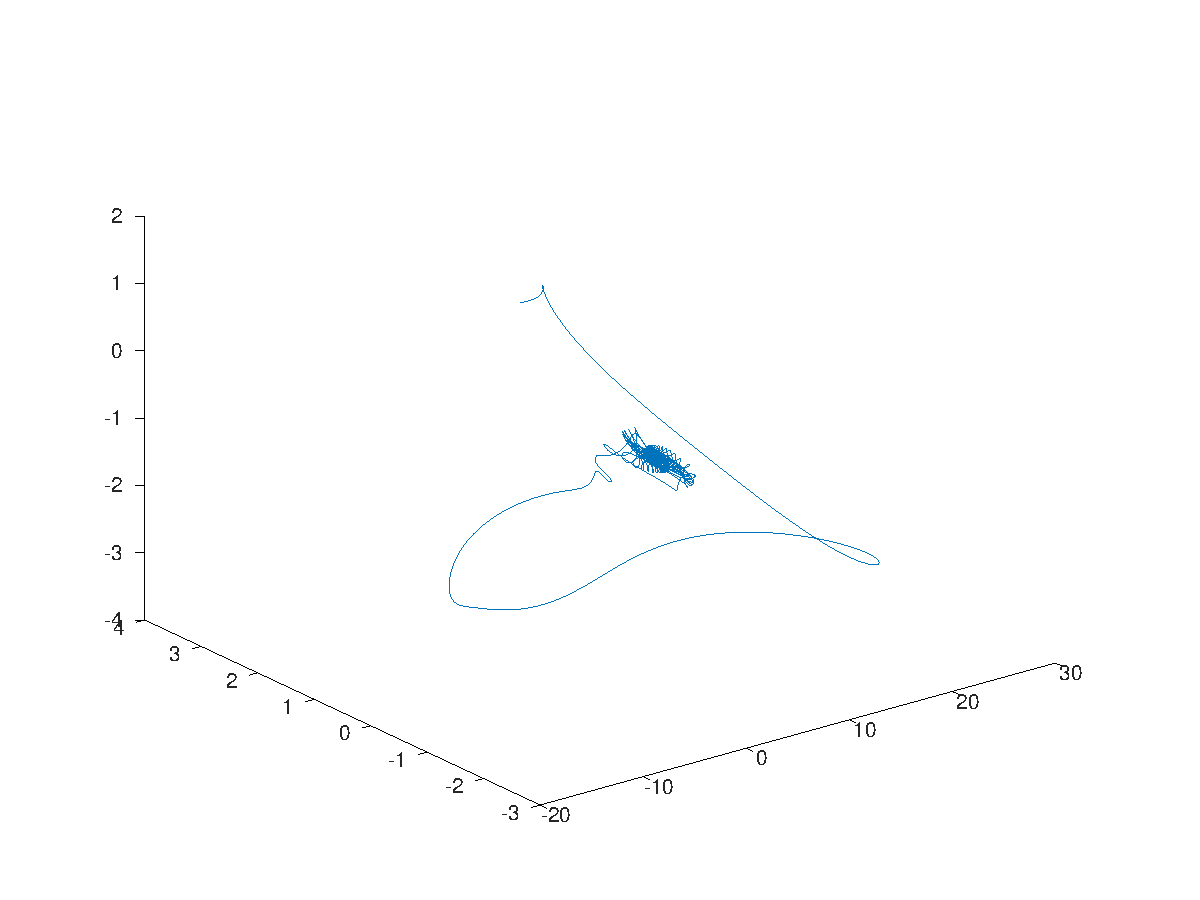
\includegraphics[width=0.49\linewidth]{{lorenz2/03-images/ord14.butterfly}.pdf}
	\caption{Lorenzssystem mit Grad 14, $t = [0,100]$}
	\label{figure:lorenz2:systemdeg14}
\end{figure}

\begin{figure}
	\centering
	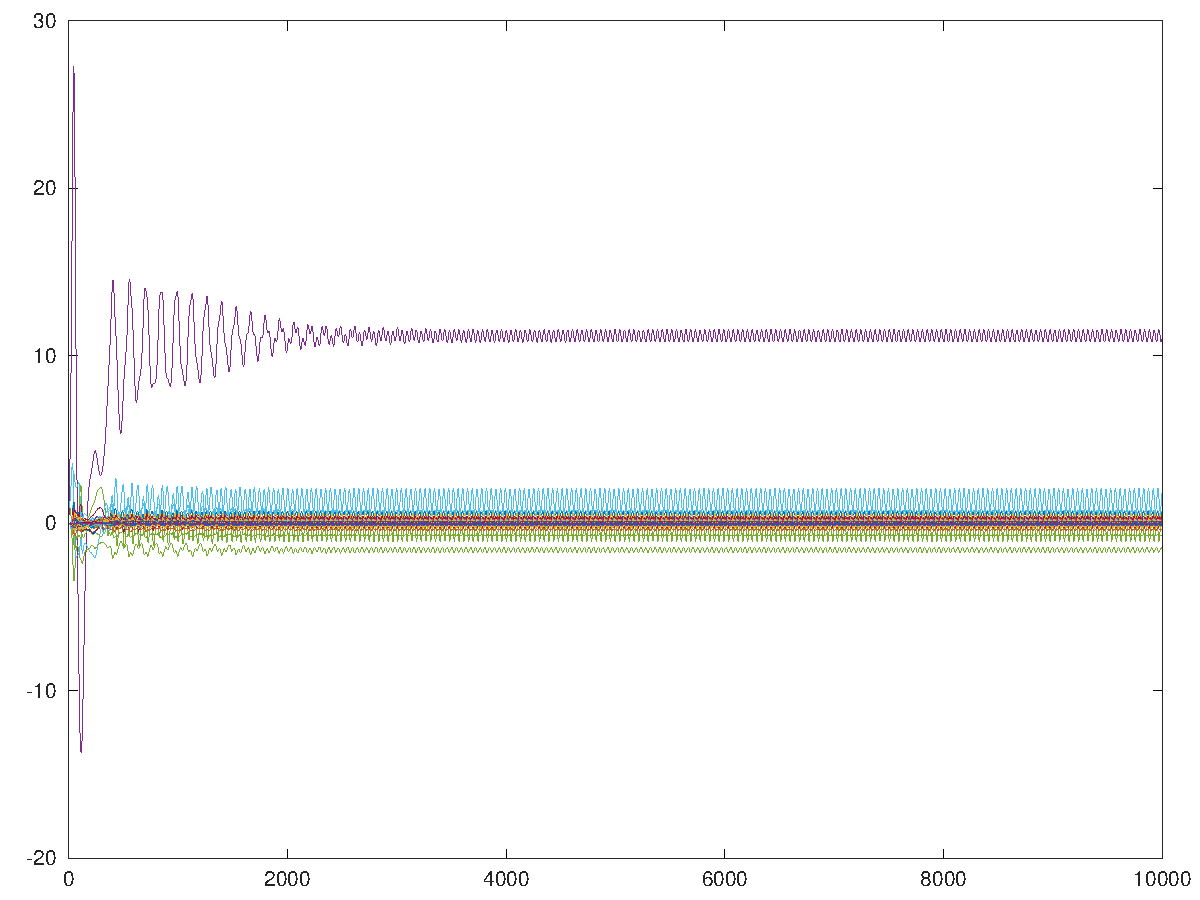
\includegraphics[width=0.49\linewidth]{{lorenz2/03-images/ord15.X}.pdf}
	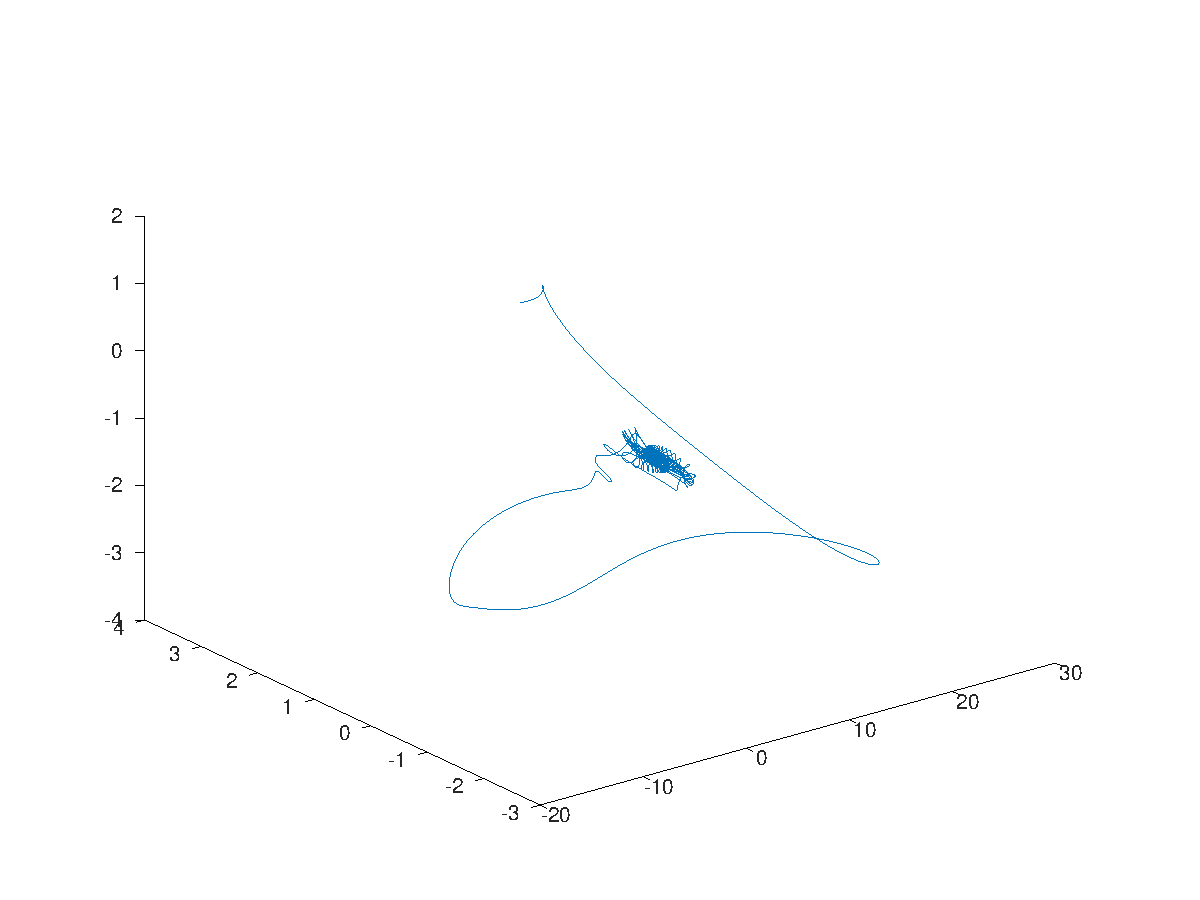
\includegraphics[width=0.49\linewidth]{{lorenz2/03-images/ord15.butterfly}.pdf}
	\caption{Lorenzssystem mit Grad 15, $t = [0,100]$}
	\label{figure:lorenz2:systemdeg15}
\end{figure}

\begin{figure}
	\centering
	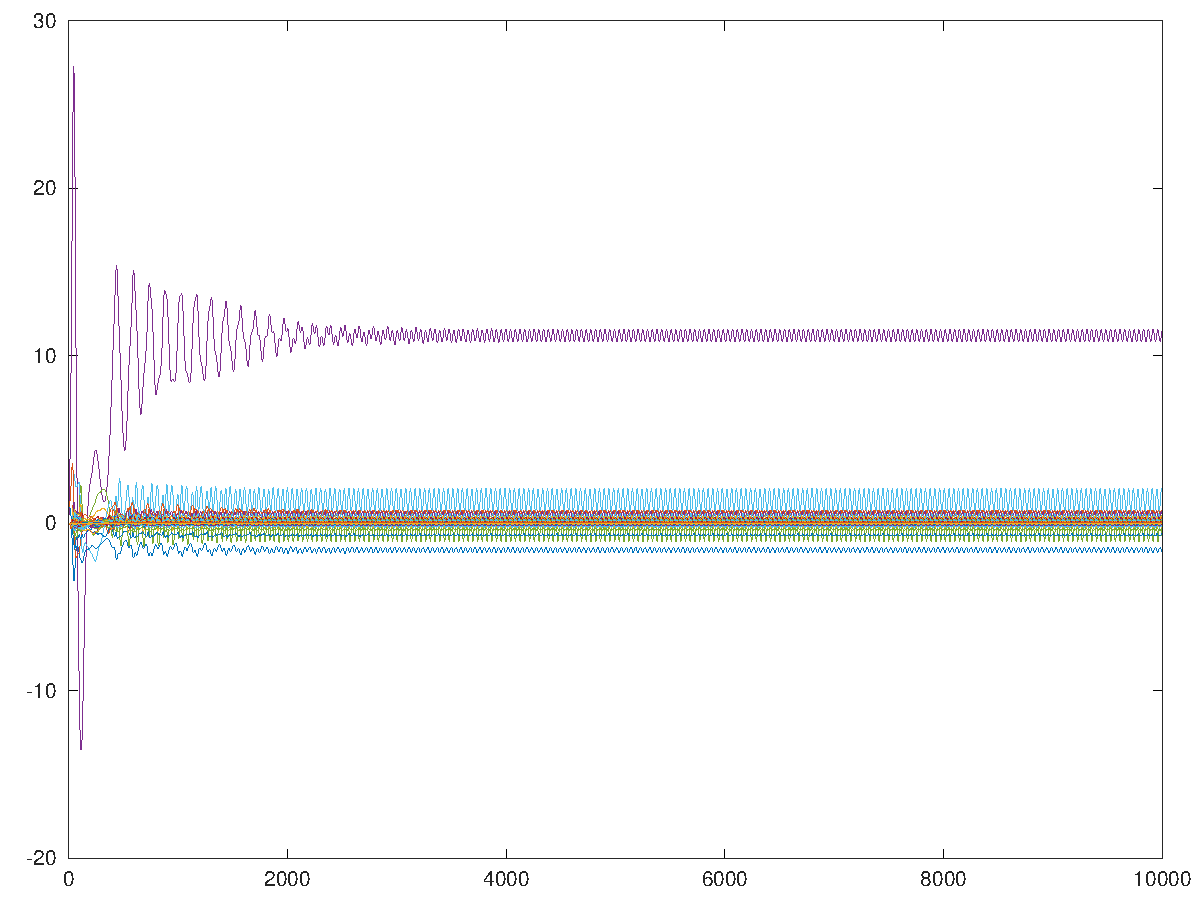
\includegraphics[width=0.49\linewidth]{{lorenz2/03-images/ord16.X}.pdf}
	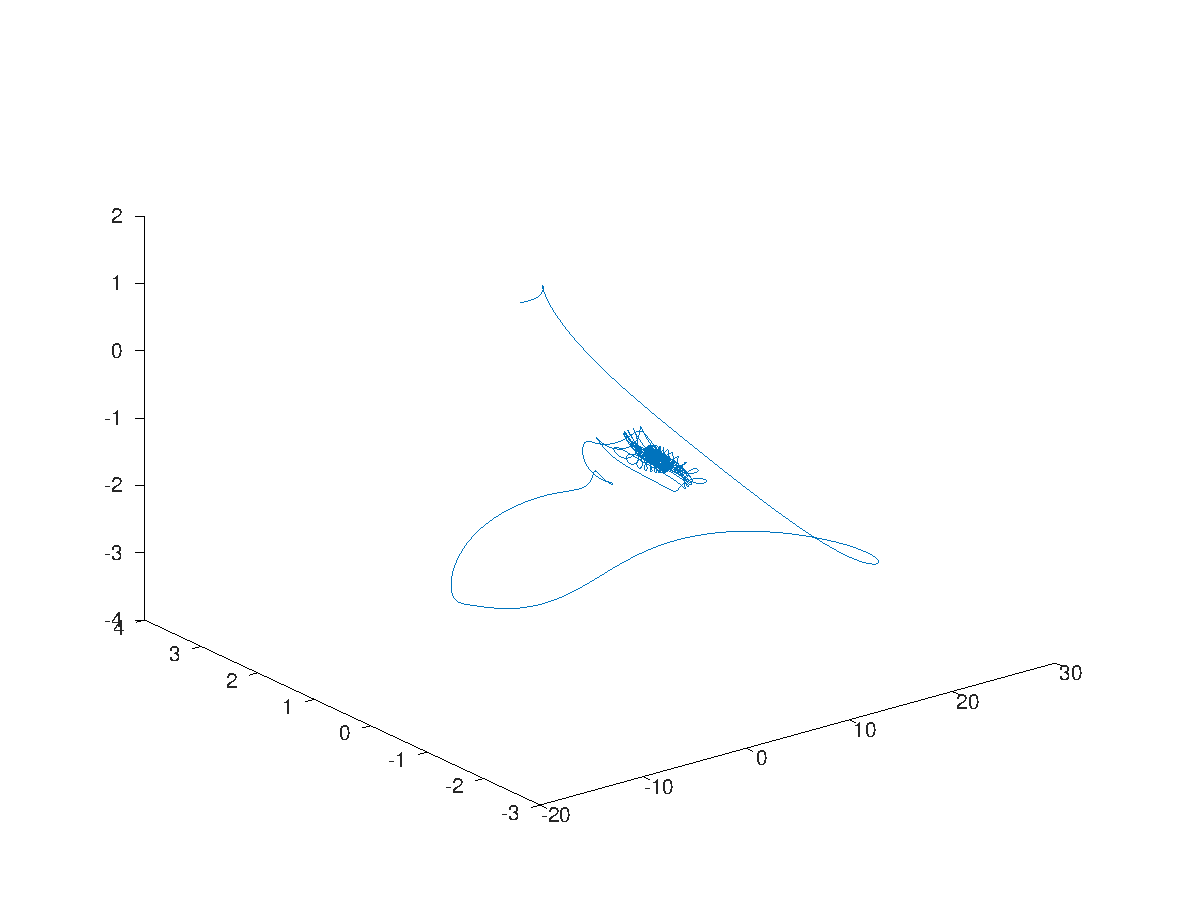
\includegraphics[width=0.49\linewidth]{{lorenz2/03-images/ord16.butterfly}.pdf}
	\caption{Lorenzssystem mit Grad 16, $t = [0,100]$}
	\label{figure:lorenz2:systemdeg16}
\end{figure}

\begin{figure}
	\centering
	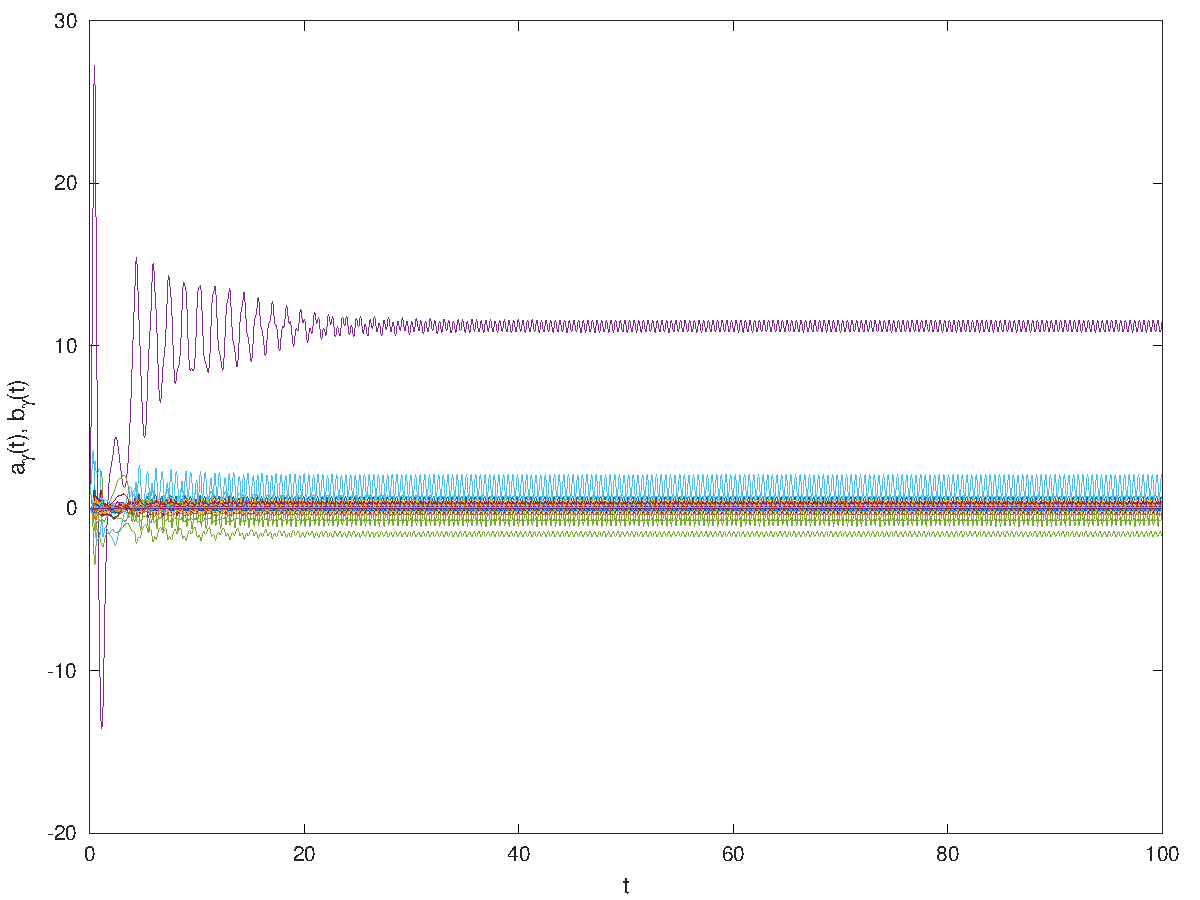
\includegraphics[width=0.49\linewidth]{{lorenz2/03-images/ord17.X}.pdf}
	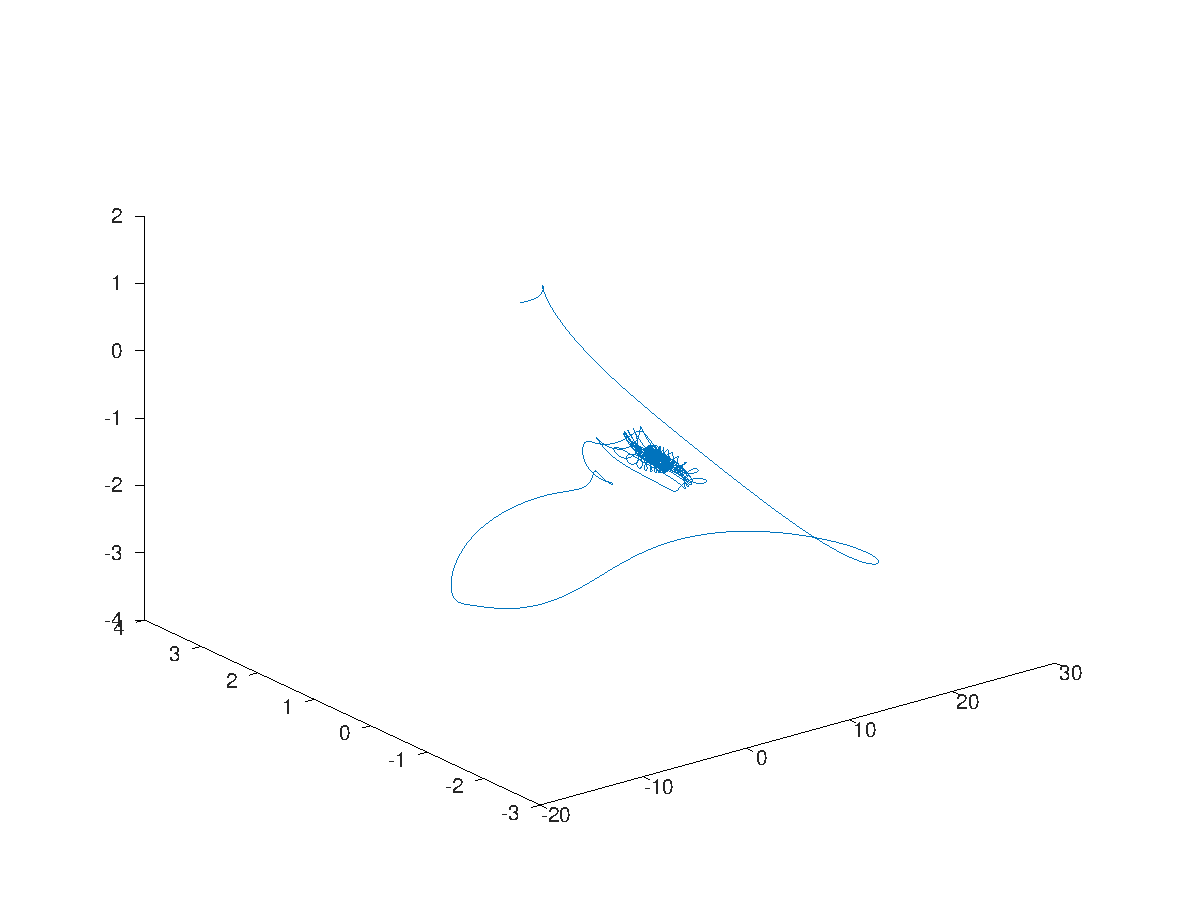
\includegraphics[width=0.49\linewidth]{{lorenz2/03-images/ord17.butterfly}.pdf}
	\caption{Lorenzssystem mit Grad 17, $t = [0,100]$}
	\label{figure:lorenz2:systemdeg17}
\end{figure}

\begin{figure}
	\centering
	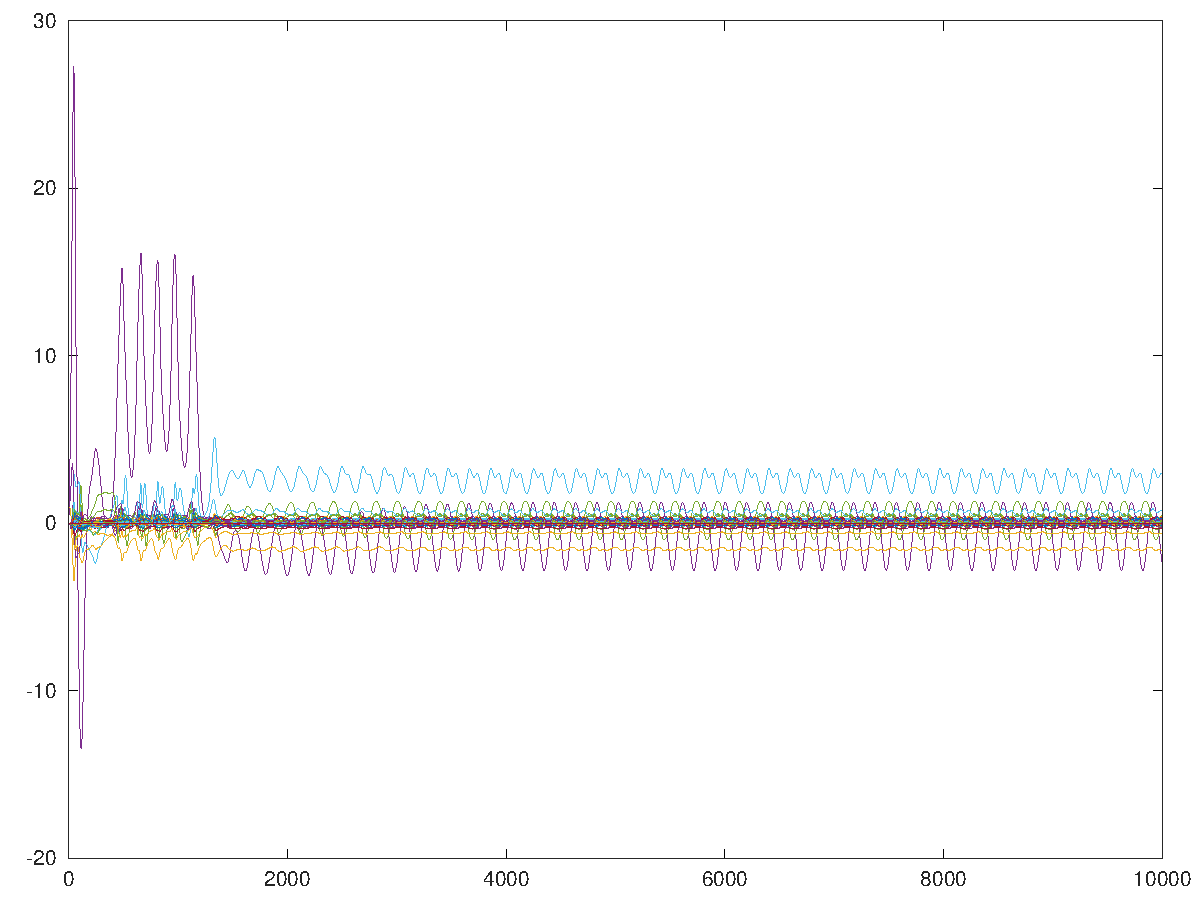
\includegraphics[width=0.49\linewidth]{{lorenz2/03-images/ord18.X}.pdf}
	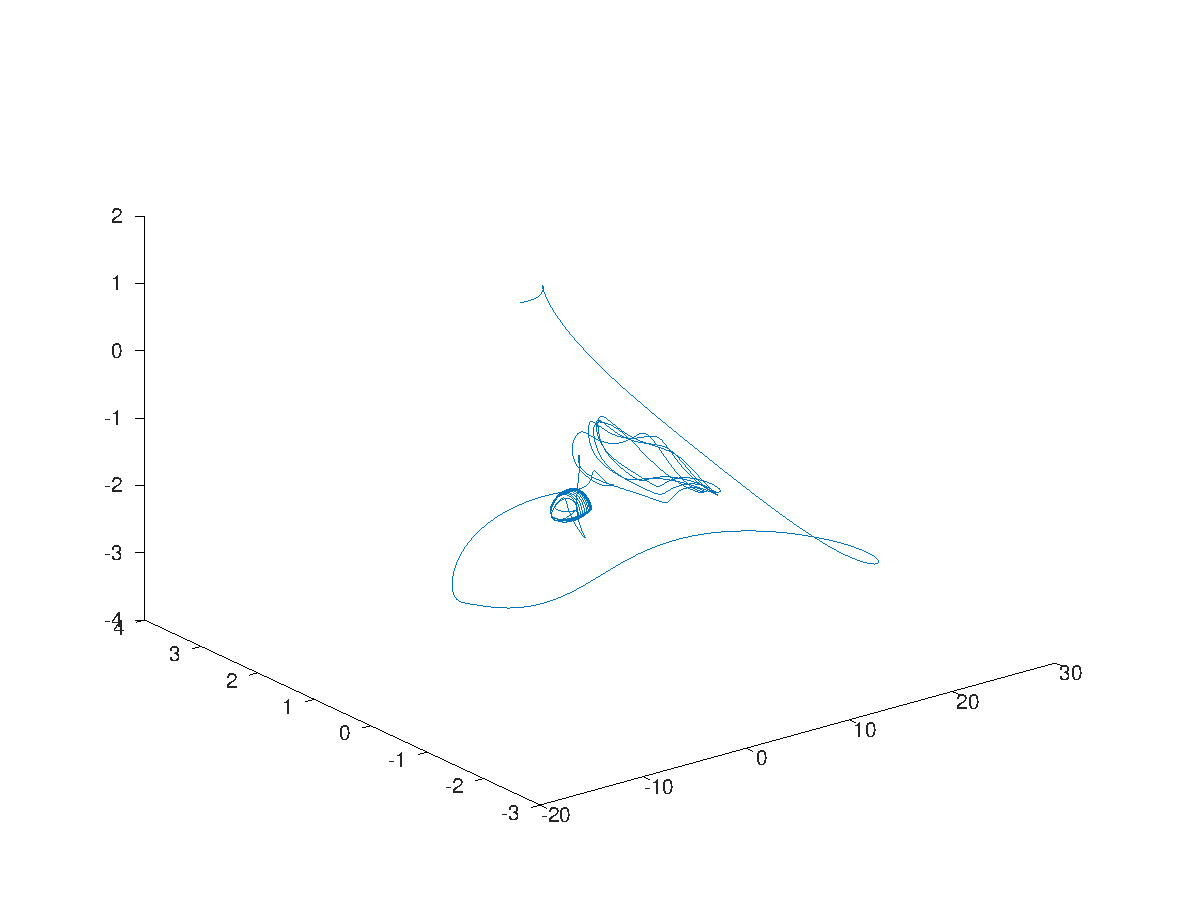
\includegraphics[width=0.49\linewidth]{{lorenz2/03-images/ord18.butterfly}.pdf}
	\caption{Lorenzssystem mit Grad 18, $t = [0,100]$}
	\label{figure:lorenz2:systemdeg18}
\end{figure}

\begin{figure}
	\centering
	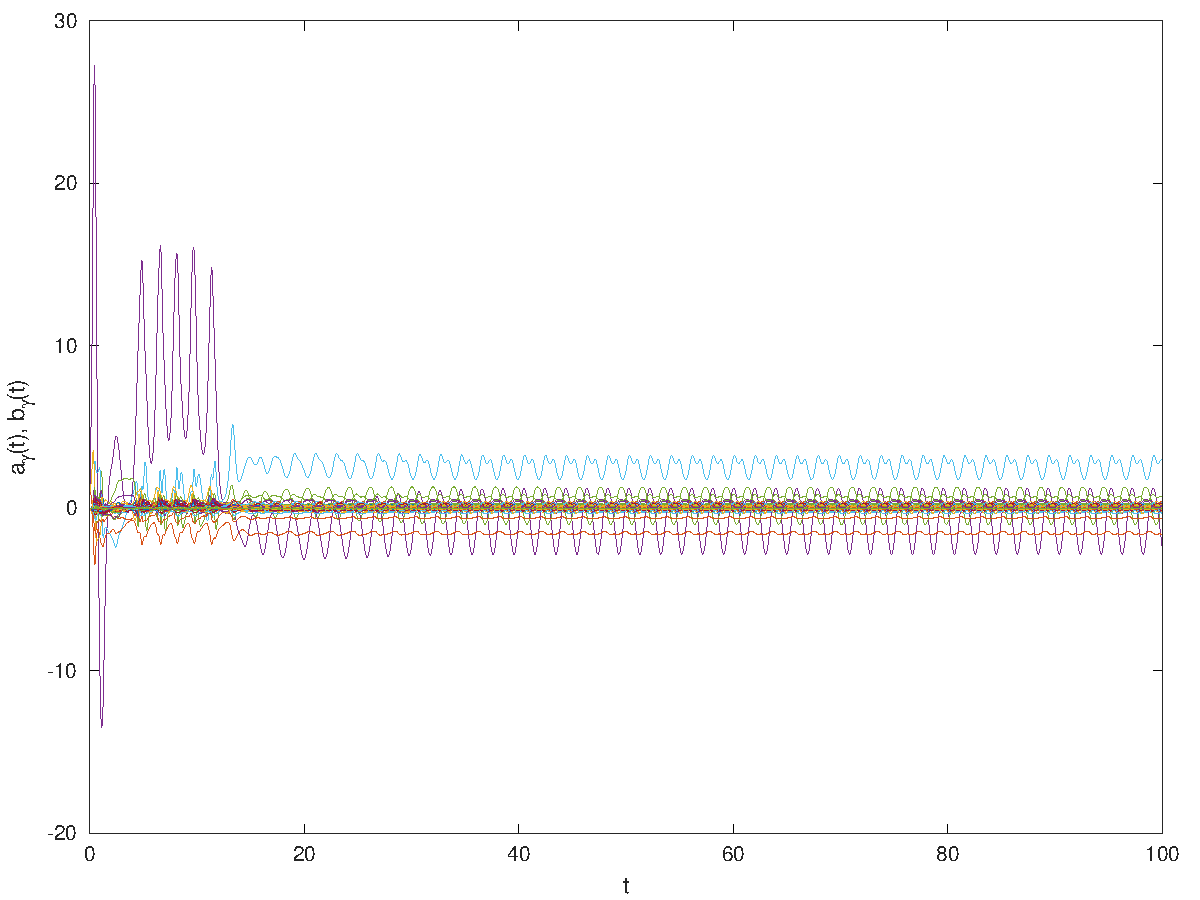
\includegraphics[width=0.49\linewidth]{{lorenz2/03-images/ord19.X}.pdf}
	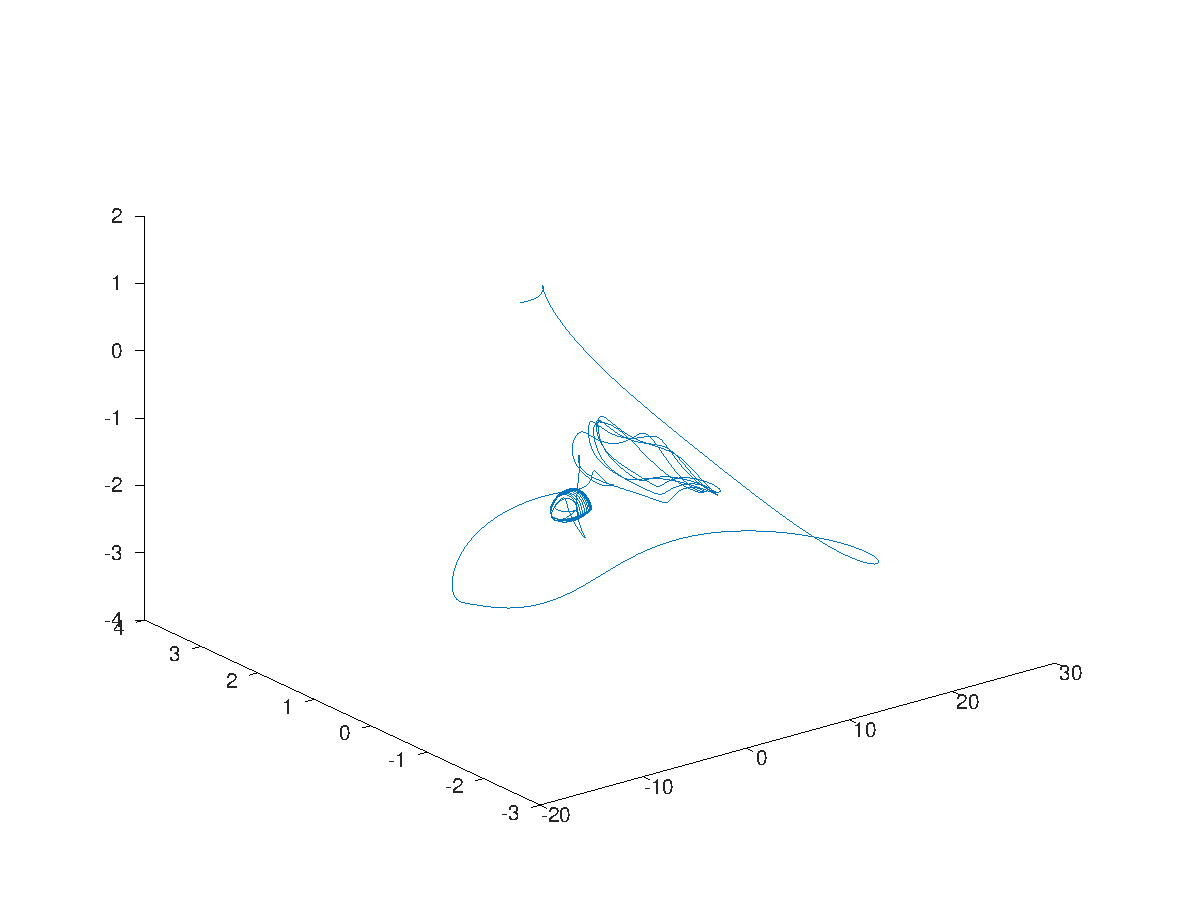
\includegraphics[width=0.49\linewidth]{{lorenz2/03-images/ord19.butterfly}.pdf}
	\caption{Lorenzssystem mit Grad 19, $t = [0,100]$}
	\label{figure:lorenz2:systemdeg19}
\end{figure}

\begin{figure}
	\centering
	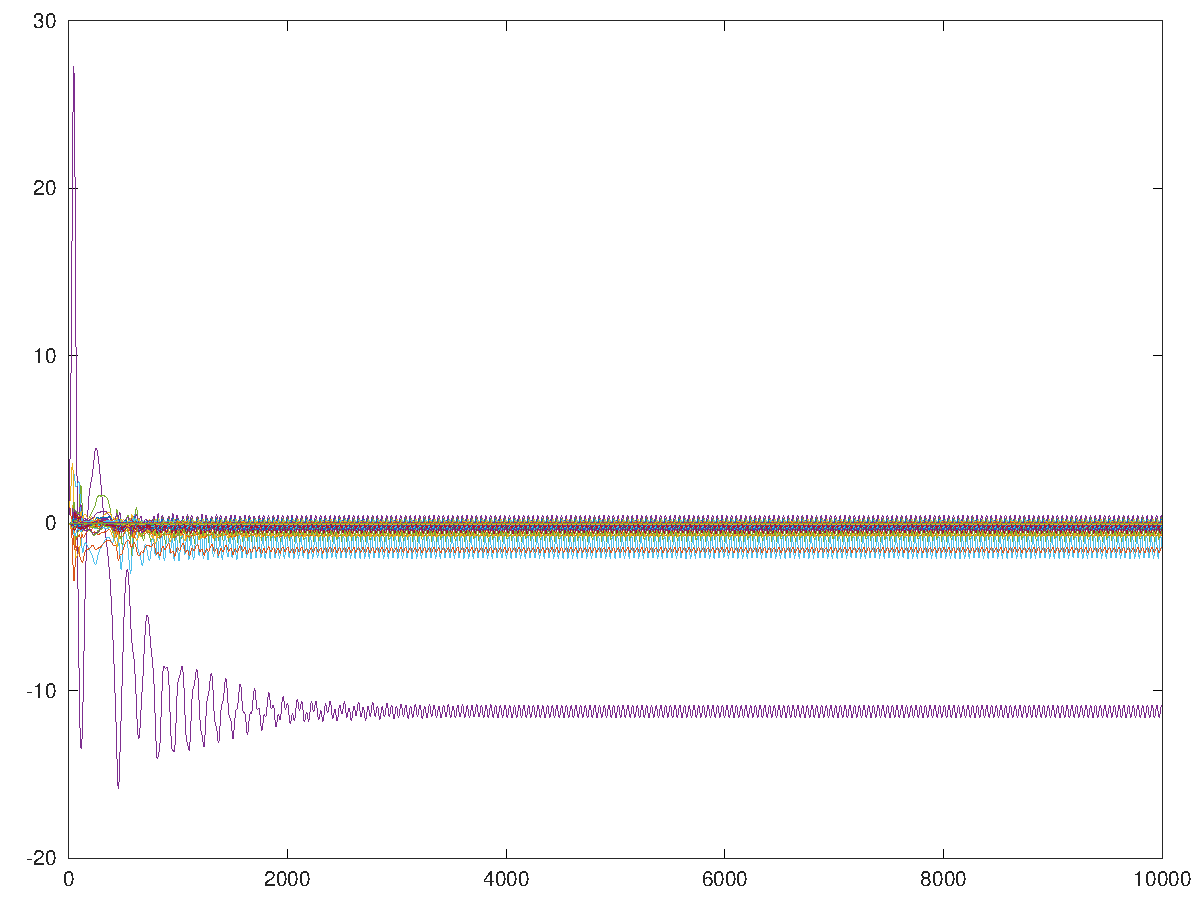
\includegraphics[width=0.49\linewidth]{{lorenz2/03-images/ord20.X}.pdf}
	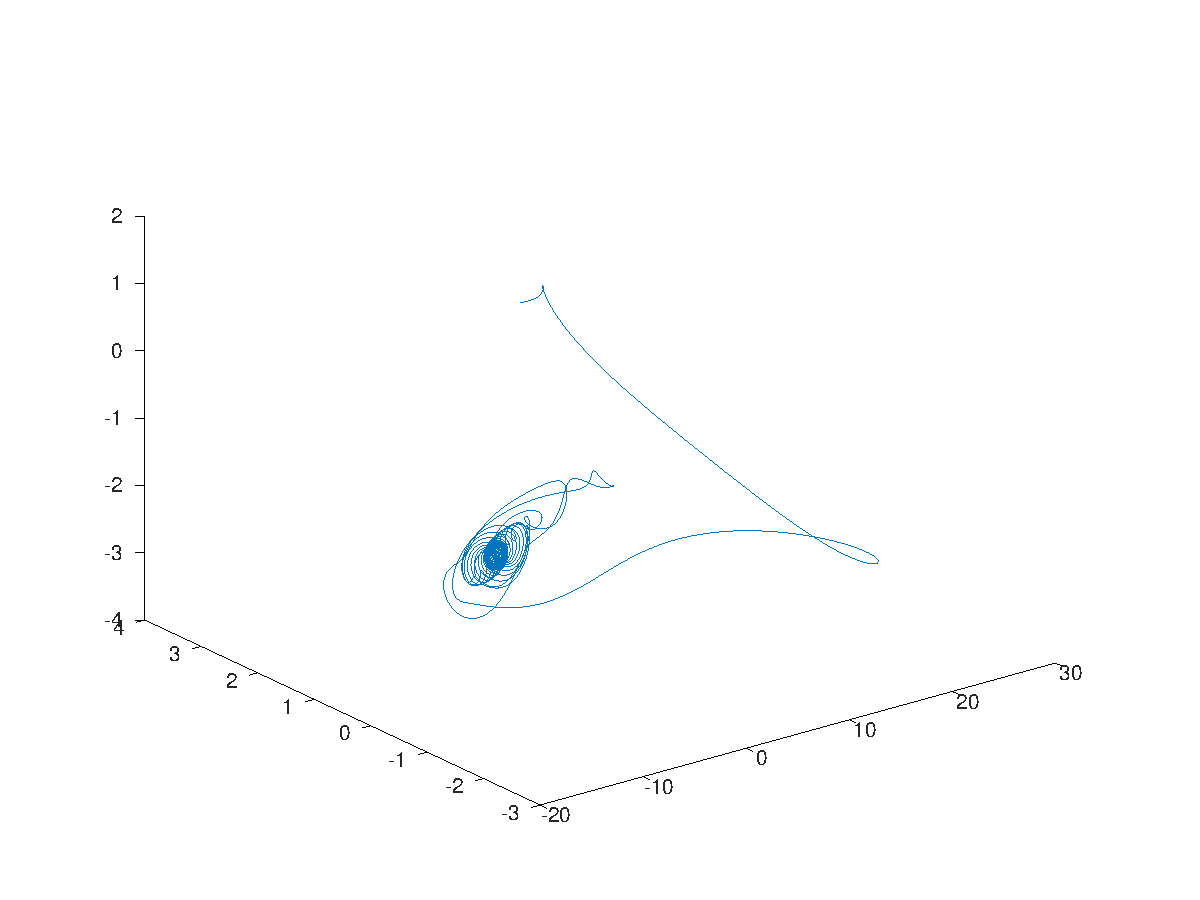
\includegraphics[width=0.49\linewidth]{{lorenz2/03-images/ord20.butterfly}.pdf}
	\caption{Lorenzssystem mit Grad 20, $t = [0,100]$}
	\label{figure:lorenz2:systemdeg20}
\end{figure}

\begin{figure}
	\centering
	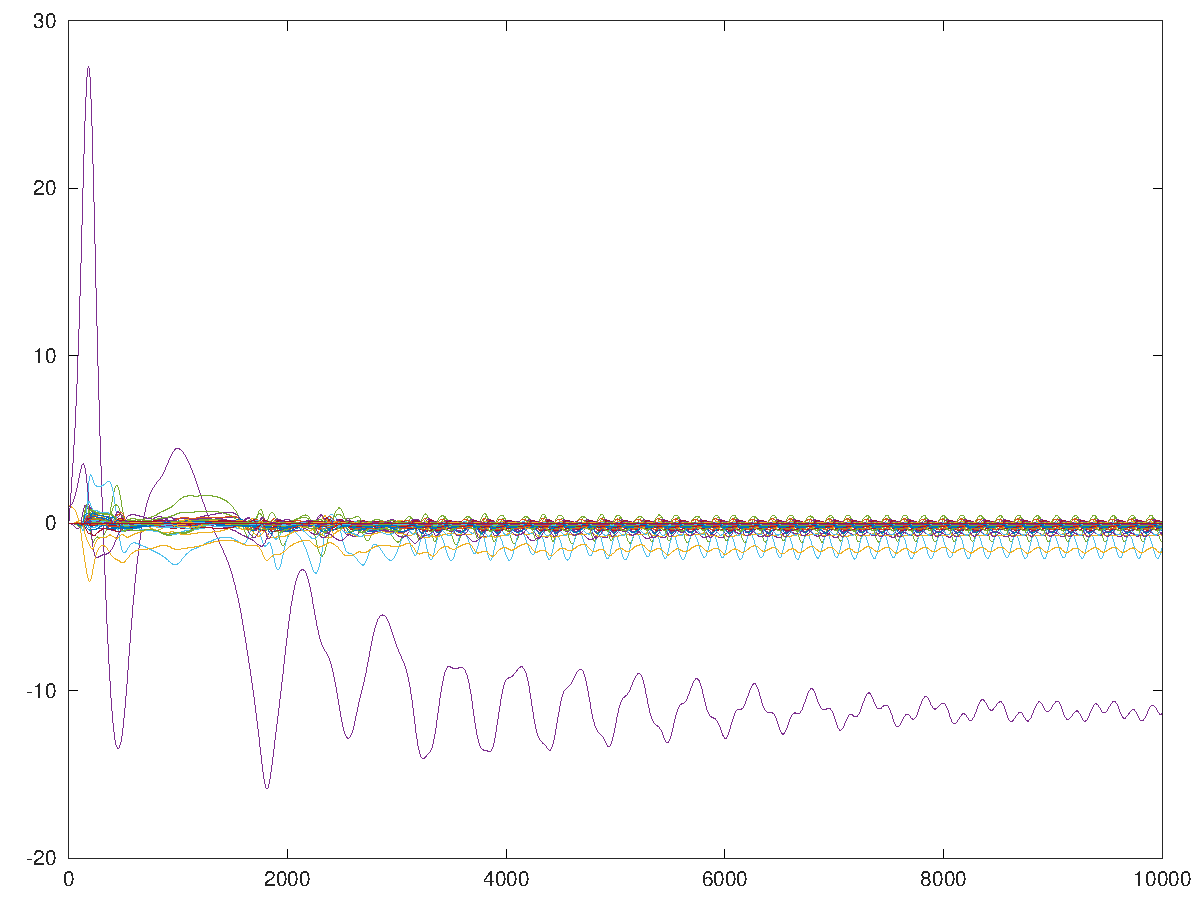
\includegraphics[width=0.49\linewidth]{{lorenz2/03-images/ord21.X.40}.pdf}
	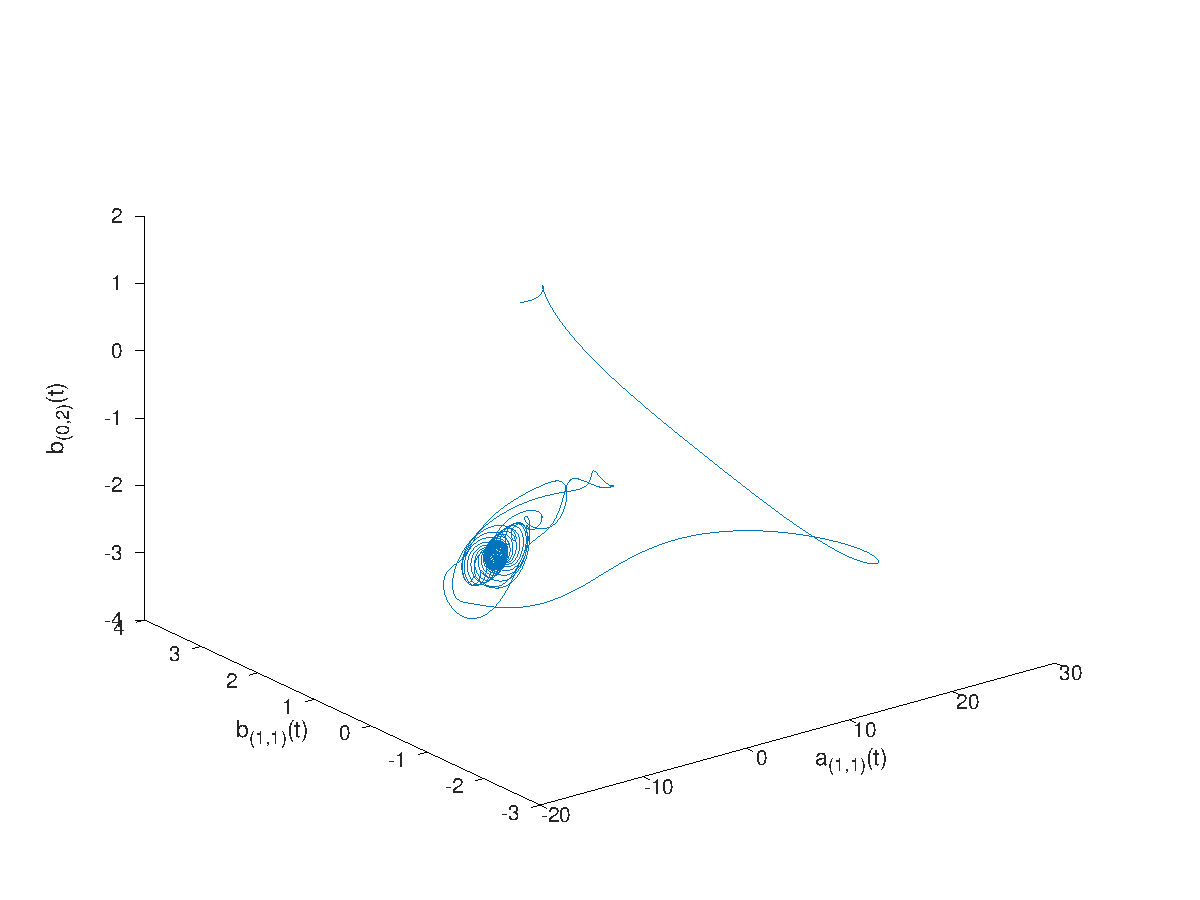
\includegraphics[width=0.49\linewidth]{{lorenz2/03-images/ord21.butterfly.40}.pdf}
	\caption{Lorenzssystem mit Grad 21, $t = [0,40]$}
	\label{figure:lorenz2:systemdeg21-40}
\end{figure}

\begin{figure}
	\centering
	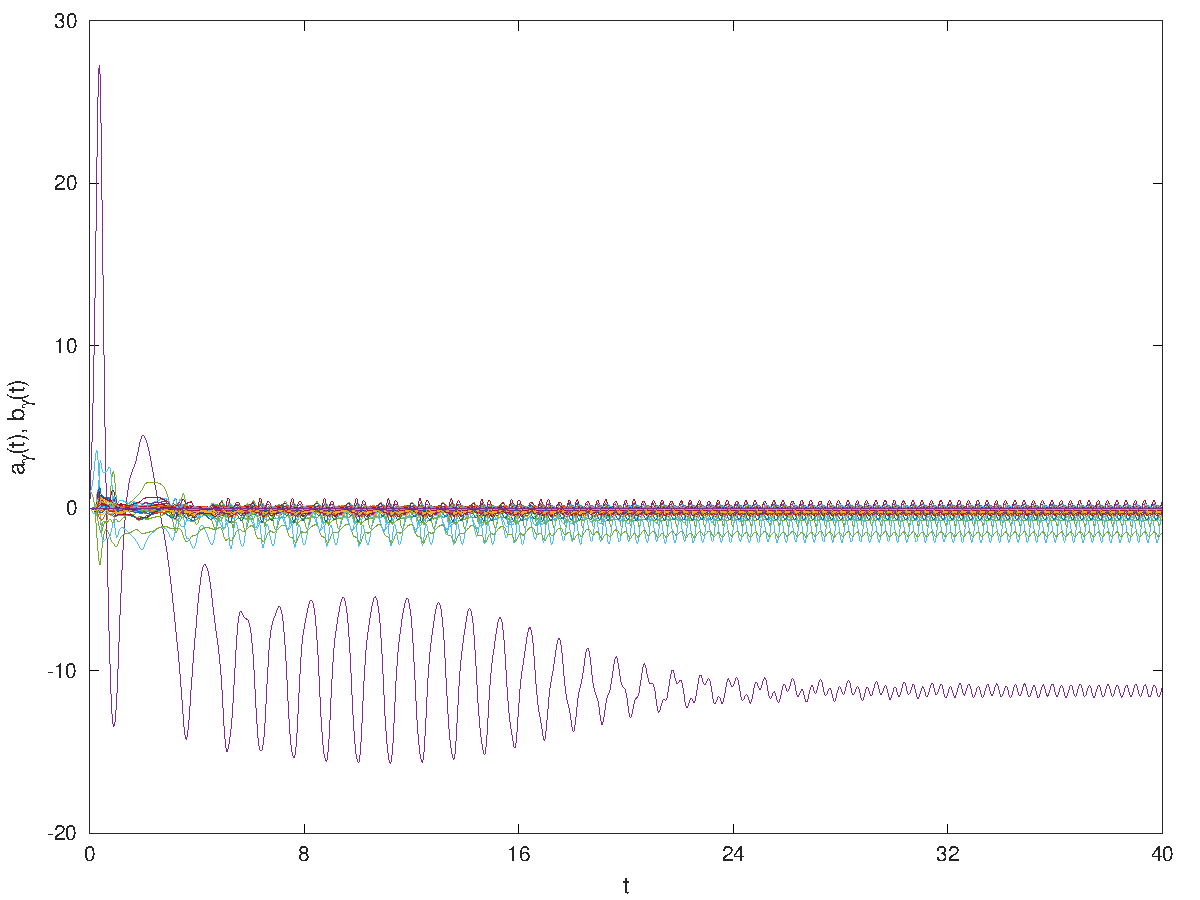
\includegraphics[width=0.49\linewidth]{{lorenz2/03-images/ord22.X.40}.pdf}
	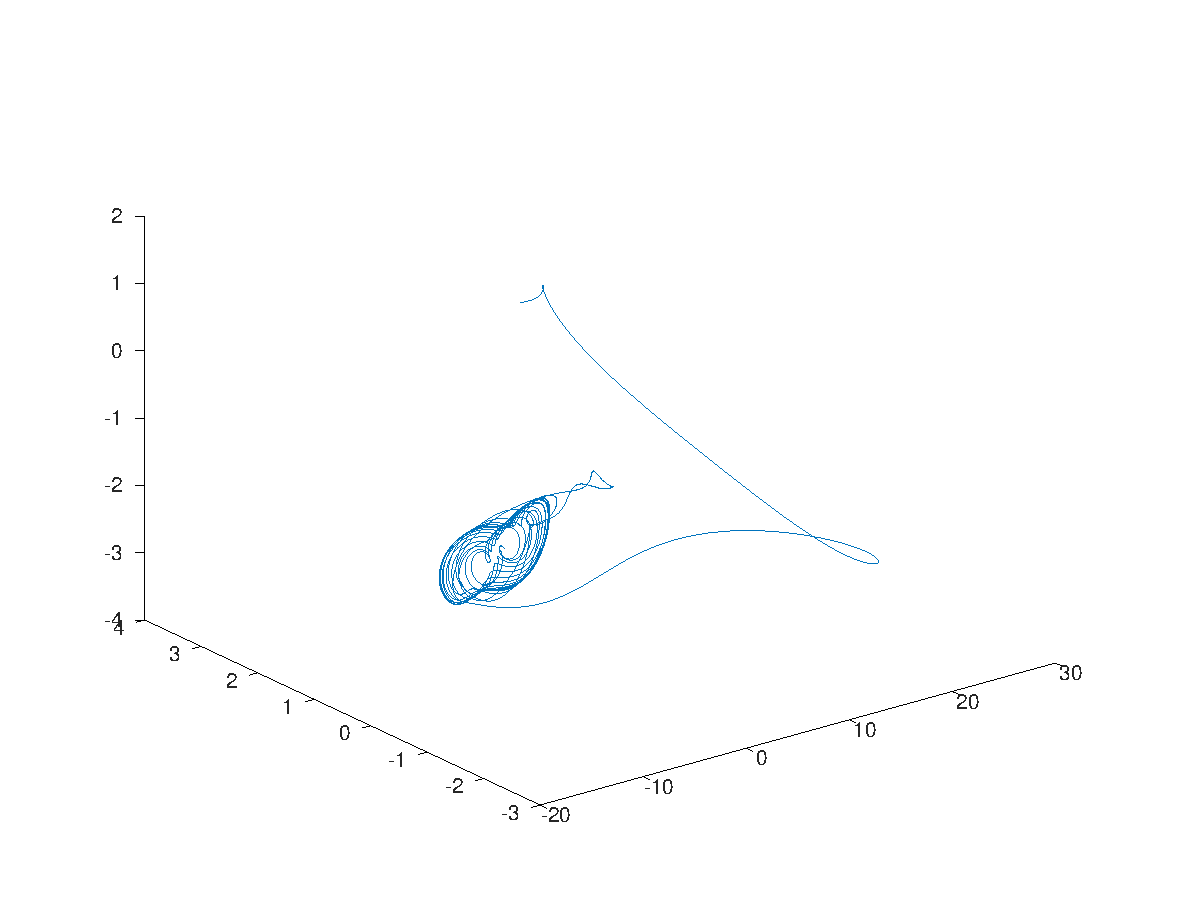
\includegraphics[width=0.49\linewidth]{{lorenz2/03-images/ord22.butterfly.40}.pdf}
	\caption{Lorenzssystem mit Grad 22, $t = [0,40]$}
	\label{figure:lorenz2:systemdeg22-40}
\end{figure}

\section{Schlussfolgerungen}
\rhead{Schlussfolgerungen}
Wir haben somit gezeigt, dass es m"oglich ist, ein h"oherdimensionales 
Lorenzsystem mittels Erweiterung der bekannten Basisfunktionen zu bestimmen. 
Wir k"onnen weiter die ben"otigten Gleichungen mittels Computer generieren und 
auswerten, auch wenn dies mit gr"osser werdendem Grad $k$ mit einem starken 
Anstieg der Laufzeit einher geht. Eine m"ogliche Verbesserung w"are 
beispielsweise eine parallele Berechnung der einzelnen gew"ohnlicher 
Differentialgleichungen, was aber nicht untersucht wurde. In einem weiteren 
Schritt m"usste zudem der Raum der Anfangsbedingungen und Parameter weiter 
untersucht werden, um zu zeigen, dass das chaotische Verhalten wirklich ab $k = 
4$ verloren geht oder ob es schlicht an den von uns gew"ahlten Anfangs- und 
Parameterwerten liegt. Zu guter Letzt k"onnte auch noch untersucht werden, was 
passiert wenn der Grad $k$ noch weiter gesteigert wird, denn es m"oglich, dass 
wir einfach noch mehr Terme ben"otigen um die ``Schmetterlingsfl"ugel'' und 
somit das chaotische Verhalten wieder zu erzeugen. Daf"ur muss allerdings viel 
Geduld mitgebracht werden.


\printbibliography[heading=subbibliography]
\end{refsection}
